% -*- coding: utf-8 -*-
\documentclass[12pt,openright]{book}

\usepackage{verbatim}

\usepackage{ifxetex}
\ifxetex
  \usepackage[bookmarksnumbered]{hyperref}
\else
  \usepackage[unicode,bookmarksnumbered]{hyperref}
\fi

\usepackage[emptydoublepage]{NKThesis}   % 中文
%\usepackage[emptydoublepage,English]{NKThesis} % 英文
\usepackage{amssymb}
\usepackage{subfigure}

\usepackage{svg}
\usepackage{algorithm}  
\usepackage{algorithmic}
\usepackage{booktabs}
\usepackage{tikz}
\usetikzlibrary{positioning, fit, arrows.meta, shapes, chains,matrix,patterns,spy,calc}

%% network
\input{./network_init.tex}



\usepackage{graphicx}
\usepackage{color}
\usepackage{pgfplots}
\usepackage{pgf-umlsd}
\usepackage{ifthen}
\usepackage[]{fp}

\usepgfplotslibrary{groupplots}
\pgfplotsset{compat=newest}

\FPset{totalOffset}{0}


% used to avoid putting the same thing several times...
% Command \empt{var1}{var2}
\newcommand{\empt}[2]{$#1^{\langle #2 \rangle}$}




%   根据需要选择 biblatex 宏包选项.
\usepackage[sorting=none]{biblatex}
% \usepackage[superscript]{cite}
\hypersetup{colorlinks=true,
            pdfborder=0 0 1,
            citecolor=black,
            linkcolor=black}
%\usepackage{tikz}
\usepackage{amsmath}
\addbibresource{nkthesis.bib}
\DeclareBibliographyCategory{cited}
\AtEveryCitekey{\addtocategory{cited}{\thefield{entrykey}}}

\includeonly{
abstract,
manual,
acknowledgements,
references,
appendices,
resume
}
\newtheorem{Theorem}{\hskip 2em 定理}[chapter]
\newtheorem{Lemma}[Theorem]{\hskip 2em 引理}
\newtheorem{Corollary}[Theorem]{\hskip 2em 推论}
\newtheorem{Proposition}[Theorem]{\hskip 2em 命题}
\newtheorem{Definition}[Theorem]{\hskip 2em 定义}
\newtheorem{Example}[Theorem]{\hskip 2em 例}
\floatname{algorithm}{算法}
\newcommand{\upcite}[1]{\textsuperscript{\textsuperscript{\cite{#1}}}}
\begin{document}

%  设置基本信息
%  注意:  逗号`,'是项目分隔符. 如果某一项的值出现逗号, 应放在花括号内, 如 {,}
%

\NKTsetup{%
  论文题目(中文) = 阿尔法雅达利:基于丰富无模型强化学习,
%   论文题目(中文)(第二行) =第二行中文题目,填无则不显示本行,
  论文题目(中文)(第二行) = 训练雅达利游戏大师,
  论文题目(英文) =  AlphaAtari: Grandmaster level in Atari using diversity , 
%   论文题目(英文)(第二行) = model-free reinforcement learning,
  论文题目(英文)(第二行) = model-free reinforcement learning,
%   论文题目(英文)(第三行) =无,
  学号           = 1711456,
  姓名          =  范嘉骏,
  学院          = 人工智能学院,
  系别          =  智能科学与技术系,
  专业           = 智能科学与技术,
  年级          = 2017级,
  论文完成时间   = 2021年5月,
  指导教师       = 郭宪\quad 副研究员,
  % 如果有校外导师则填写校外导师。没有填无
  校外导师      =无,
%   校外导师     = 罗翔\quad 教授(张三大学),
  }






% -*- coding: utf-8 -*-


\begin{zhaiyao}
2015年深度学习和强化学习的首次结合在雅达利49类游戏上取得巨大成功,但是强化学习算法应用的过程中仍存在大量的问题,如算法稳定性差,可扩展性差等,这些问题阻碍了其进一步的应用。举例来说,学者常常会在雅达利平台上测试算法的性能,而传统的强化学习算法只能解决一些简单的游戏,并且在不同的游戏中其表现差距很大。为了进一步提升强化学习算法的学习效率和泛化性能,文章提出了名为AlphaAtari的强化学习算法,在保证算法高效性的同时,极大的提升算法的稳定性和可扩展性。
为了达到这种效果,文章首先提出一套完整的无模型强化学习统一框架,然后通过引入策略族来丰富文章的采样策略。此外,文章针对性的设计了面向耦合多参数的自适应控制器来自动地调整算法中的各种具有强关联性的超参数。实验表明文章的算法在雅达利全部57个游戏中在人类归一化平均得分这一指标上超越了当前的得分最高的算法Agent57,意味着这项工作使文章向实现通用人工智能迈出了坚实的一步。
\end{zhaiyao}




\begin{guanjianci}
强化学习;深度学习;瓦砾编码;数据分析
\end{guanjianci}



\begin{abstract}
In 2015, the first combination of deep learning and reinforcement learning achieved great success in Atari 49 games, but there are still a lot of problems in the application of reinforcement learning algorithms, such as poor algorithm stability and poor scalability. These problems hinder its further application. For example, researchers often test the performance of algorithms on the Atari platform, while traditional reinforcement learning algorithms can only solve some simple games, and their performance varies greatly in different games. In order to further improve the learning efficiency and generalization performance of the reinforcement learning algorithm, this paper proposes a reinforcement learning algorithm called AlphaAtari, which greatly improves the stability and scalability of the algorithm while ensuring the efficiency of the algorithm.
In order to achieve this effect, this paper first proposes a complete unified framework for model-free reinforcement learning, and then enriches the sampling strategy of this article by introducing a strategy family. In addition, this paper specifically designs an adaptive controller for coupled multi-parameters to automatically adjust various hyperparameters with strong correlation in the algorithm. Experiments show that our algorithm has achieved the highest average human normalized  scores in all 57 games of Atari, surpassing the current highest-scoring algorithm Agent57, and has taken a solid step towards the realization of general artificial intelligence.
\end{abstract}



\begin{keywords}
reinforcement learning; deep learning; tile coding; data mining
\end{keywords} 

\addcontentsline{toc}{chapter}{目\quad录}
\tableofcontents

% -*- coding: utf-8 -*-
\chapter{绪论} 
\label{chpt:A}


\section{简介}
%% 简单的介绍

强化学习(Reinforcement Learning, RL)是由索恩迪克(Thorndike)\upcite{thorndike1898animal}对猫的行为进行的观察实验中,受到动物通过反复试错(Trial and Experiment, TE)的启发而被首次提出。1954年,明斯基(Minsky)\upcite{minsky1954theory}成功地自主设计并提出了第一个被人们称为随机神经元器的模拟器(Stochastic Neural-Analog Reinforcement Calculators, SNARCs)的神经计算机,这台计算机可以通过模拟小鼠的大脑神经元的活动来解决迷宫难题(Maze Puzzle)。从SNARCs开始,基于TE的学习已经达到了一种可计算的阶段\footnote{在SNARCs之前,基于TE的学习大多数是关于动物行为的观测实验。}。大约20年后,卡罗夫(Klopf)\upcite{klopf1972brain}首次将人体心理学中的时间差分的学习机制引入应用到 TE学习的一个计算图模型中。这一跨时代的结合使得TE学习模型可以应用到一些大规模问题中。1989年,瓦克因(Watkins)和戴因(Dayan)\upcite{watkins1992q}将贝尔曼方程和马尔科夫决策过程在内的一些最优控制理论\upcite{bellman1952theory}与时间差分结合在一起,首次提出了目前广为人知的强化学习算法:Q-学习(Q-learning)。从那时起,Q-learning算法
逐渐地应用于解决各种现实问题。然而,在类似机器人控制、视频游戏等含有高维信息的任务中,Q-learning的计算量随着输入的增加而指数级扩大,所以当时Q-learning算法仍然无法很好的处理这类问题。这种超出了传统计算机的可计算空间的问题常常被称为维度灾难。2015年Mnih\upcite{mnih2015human}等人通过将深度学习(Deep Learning, DL)与Q-learning结合在一起,在一定程度上缓解了维度灾难的问题,并且开启了深度强化学习(Deep Reinforcement Learning, DRL)的时代。从那时起,DRL已经成为人工智能领域的一颗璀璨的明珠。为了更好地便于学习和理解,我们将在强化学习和发展中对于一些具有里程碑意义的事情进行整体总结并纳入到了\textbf{图\ref{Fig:rl milestone}}中。

\begin{figure}[!t]
	\centering
	\subfigure{
		\centering
		\includegraphics[scale=0.5]{photo/chapter1/1.1.pdf}
	}
	\caption{强化学习发展里程碑}
	\label{Fig:rl milestone}
\end{figure}

正如我们所提到的,RL起源于生物学家和心理学家关于动物行为学和心理学的研究,其本质就是对动物学习行为和过程的一种仿生计算(Bionic Computing),因此RL完全可以通过模仿人类的学习能力,以选择能够适应环境变化并在与环境的互动中可以获得长期利益的行动。可以看出,RL的目标是训练出与人类智力水平相当,甚至超越人类水平的智能体(Agent)。例如,RL已经在机器人(Robotics)和自动控制(Automatic Control)等领域具有广泛的应用。1992年,马哈德瓦(Mahadevan)和康奈尔(Connell)\upcite{mahadevan1992automatic}设计出了可以自主推动立方体的机器人。1997年,沙尔(SChaal)\upcite{schaal1997learning}创建了一个可以高效解决倒立摆(Inverted Pendulum)平衡任务的机器人。同样是1997年,布巴赫(Benbrahim)与富兰克林(Franklin)\upcite{benbrahim1997biped}制造了一种双足机器人(Biped Robot),可以在
陌生环境中学会走路。2009年,雷德曼(Riedmiller)等人\upcite{riedmiller2009reinforcement}成功构造了一支足球机器人联队。2013年米娜(Muelling)\upcite{mulling2013learning}等人训练了可以打网球(Tennis)游戏的机器人。

DRL开始的标志性事件就是Mnih等人\upcite{mnih2015human}在2015年首次提出DQN结构,并利用DQN在49款雅达利游戏(Atari Games)\upcite{bellemare2013arcade}上训练出具有人类专业玩家水平的智能体。2016年谷歌的DeepMind\footnote{DeepMind是一家致力于实现通用人工智能的高科技公司。}创建了一个从零开始自学成才的围棋智能体训练算法AlphaGo\upcite{silver2016mastering},该智能体击败了包括中国柯洁和韩国李世石在内的国际知名围棋选手。DRL同时也被用于解决机器人控制问题如MuJoCo\upcite{duan2016benchmarking}和3D迷宫类游戏\upcite{beattie2016deepmind}。2017年,OpenAI训练得到了一个可以在多人Moba类游戏Dota2\upcite{berner2019dota}
达到大师级水平的智能体,相较于棋盘类游戏,DOTA2环境更为复杂,更具有挑战性。此外,DRL在自动控制领域的应用使得自动驾驶领域也得到了空前的发展。更重要的是,DRL已经成为解决现实中复杂问题的一种具有广泛应用前景的标准范式,同时为通用人工智能领域的发展做出了巨大贡献。

与传统的监督学习(Supervised Learning, SL)和传统的无监督学习( Unsupervised Learning, UL)相比,强化学习研究的主题别具一格。从历史上看,自1960年以来,SL和RL一直存在着概念混淆的问题。直到1981年萨滕(Sutton)和巴托(Barto)\upcite{sutton1998introduction}对于强化学习标准的定义,我们才逐渐对两种学习方法之间的差异有所了解。简而言之,SL方法通常从提前定义的固定格式的输入输出样本数据中进行学习,而强化学习通过与未知环境交互自主获取反馈信号进行学习。所以如果直接将SL的方式用于RL任务中,几乎不可能通过人工收集现实任务中的所有可能行为来得到每一个状态点对应的正确反馈信号。然而,RL智能体可以通过执行TE的过程获取经验,然后随着时间推移不断的提升自身的智能水平。此外,我们需要理解RL并不是一种UL算法。UL算法通常学习和搜寻输入信息中隐藏的关联或数据结构,
而这并不是RL算法的目的。简而言之,RL是一种目标导向的学习方法,也就是说RL方法构建了一种学习模型该模型明确指定了学习的目标和学习的过程,然后智能体通过最大化长期收益来逐步提升其智能水平。最后,还需要说明的是DRL和DL在处理的任务等方面也存在明显的不同。DL使用不同的神经网络(Neural Networks, NN)进行表征学习(Representation Learning),主要希望解决不同级别的特征提取(Feature Extraction)和特征抽象(Feature Abstraction)等任务\upcite{deng2014deep}。DRL利用DL解决高维数据的感知任务,然后基于抽象感知来进行智能体训练,这种结合的方式使得DRL成为解决现实问题的一种极具前途的方法。

我们中我们主要就如何在雅达利游戏中训练得到大师级水平的智能体设计了一套全新的强化学习算法,在本章接下来的几节中我们将逐步介绍我们的研究动机、主要贡献,并在最后一节总结我们这篇文章的组织架构。
\section{研究动机}
%% 为什么要研究这个问题

针对单个智能体的强化学习算法(Single Agent Reinforcement Learning, SARL)主要有两大分支:第一类就是无模型算法(Model-Free Reinforcement Learning, MFRL),第二类是基于模型的算法(Model-Based Reinforcement Learning, MBRL)。而MFRL算法又是当前SARL算法研究的核心部分。MFRL算法的核心目标是学习一种策略,该策略能够直接从智能体与环境交互的样本中最大化折扣累计回报(Discount Cumulative Return)。而MFRL主要可以划分为两类:基于值函数的强化学习(Value-Based Reinforcement Learning, VBRL)方法\upcite{watkins1992q},VBRL算法中的智能体通过
DL预测采取某种行为的期望价值\upcite{riedmiller2005neural},常常被称为行为值函数(Action Value Function),然后根据预测的行为值函数选择最优动作;另外一类就是基于策略优化的算法(Policy-Based Reinforcement Learning, PBRL),PBRL算法中的智能体可以直接学习每个状态下的最优的策略分布。尽管以往的工作将两类方法构建起了一定的关联\upcite{nachum2017bridging},但是这种关联远远称不上统一,所以我们仍然需要一个全新的MFRL统一框架\upcite{schulman2017equivalence}。

简单来说,VBRL通常使用贝尔曼最优算子(Bellman Optimal Operator)进行值函数迭代,希望使用该算子能够将值函数向着更优质的方向转变\footnote{在\textbf{第五章\ref{sec: Training data importance analysis}}中我们将会介绍DRL中使用贝尔曼最优算子需要具备一定条件才能向着更优质的方向迭代。}。当我们参数化策略出现问题时,我们通常会使用VBRL的方法进行学习。在这种情况下,学习过程将改进算子(Improvement Operator)和投影算子(Projection Operator)交织在一起,通常会增大算法的不稳定性。

这种观点是围绕VBRL方法的特点提出的,而在PBRL的方法中却很难发现类似的结论,相反我们通常使用期望收益对策略参数的梯度上升\upcite{williams1992simple}来进行策略优化。尽管在使用足够小的迭代步长时,我们仍然能够在一定程度上保证收敛性,但是我们仍然没能够找到一种可以统一二者的框架\upcite{schulman2015trust}。

简而言之,目前的MFRL算法仍然没有能够完成阶段性的统一,并且大量的RL算法无法真正的广泛应用到不同的场景中。所以,我们主要探究如何得到一种统一的框架将VBRL和PBRL相统一,并在此基础上探究如何提升强化学习算法的鲁棒性、稳定性、适用范围等。
\section{主要贡献}
%% 我们研究的产出和贡献
正如上一节提到的我们的核心目标是设计一套能够统一MFRL的算法框架,我们将其称为AlphaAtari。我们使用该框架在雅达利游戏开源测试平台中以200M的极低训练量就超越了包括Agent57\upcite{badia2020agent57}、NGU\upcite{badia2020never}、R2D2\upcite{kapturowski2018recurrent}等目前最强算法。在这一节我们总结了我们研究的主要贡献:
\begin{enumerate}
    \item 我们针对off-policy学习中如何控制样本丰富度和如何获取优质样本等问题,首次提出了基于宽度策略族的强化学习方法。首次将熵群、策略群等概念引入到强化学习中,并且基于不同的待优化空间提出了多种策略群的构造方法。
    \item 我们首次将策略表示为优势函数的玻尔兹曼函数形式,使得策略具有了完全显式的形式,基于此我们结合策略群构造了如\textbf{式\eqref{Equ: diversity pi equations}}所示的一套完整的无模型强化学习统一框架。
    \item 我们针对机器学习中的超参数优化问题设计了多套完整的自适应控制器。从最基础的一个超参数的自适应控制器到任意多个具有耦合关系的超参数控制器,我们都给出了多种可行方案。
    \item 与其他的控制器不同,我们创新性的提出了基于投票的方法使得我们可以将任意多的超参数控制器结合起来以提升控制器的稳定性和收敛速度。为了提升算法的实时性我们还提出了可以在线学习的超参数控制器以适应更多的应用环境。
    \item 通过将带策略群的无模型强化学习统一框架和含多耦合超参数的自适应控制器相结合,我们得到了完整的AlphaAtari算法。此外,我们还通过AlphaAtari训练得到了大量在雅达利游戏中取得大师级水平的智能体。显而易见,我们的工作使得人类距离实现通用人工智能更进一步。
\end{enumerate}
\section{组织架构}

这一节中我们主要介绍我们的组织架构。首先,我们在\textbf{\ref{Chpt: Reinforcement Learning}}中主要介绍RL常见的分析框架即马尔科夫决策过程(Markov Decision Process, MDP)、贝尔曼方程(Bellman Equation)以及常见的RL方法等。而在接下来的\textbf{\ref{Chpt: experiment intro}}中,我们将对我们的实验平台做详细的介绍。同时我们还讨论了不同指标来评价不同算法的优劣程度的可行性,我们将会在\textbf{\ref{Chpt: experiment analyze}}的实验中展示AlphaAtari在这些指标上的表现。\textbf{\ref{Chpt: auto-ml}}中我们主要介绍如何将最简单的RL算法多臂赌博机(Multi-Armed Bandits)设计一套完整的超参数自适应控制器,包括单个超参数的控制器、任意多个超参数的控制器、以及任意多个具有关联性的超参数的控制器等。随后,在\textbf{\ref{Chpt: diverisity pi}}中我们将逐步介绍AlphaAtari算法的完整流程。我们首先针对训练数据的重要性展开分析,然后基于分析提出策略族优化的RL基本框架。进一步介绍我们针对AlphaAtari设计的采样策略控制器,最后我们给出了算法实现的整体流程。\textbf{\ref{Chpt: experiment analyze}}中,我们针对雅达利游戏平台中全部57种雅达利游戏做了充足的实验,实验结果表明我们的算法具有超强的采样效率,并且在200M的训练量下就击败了目前分数最高的算法Agent57,并且我们还分析了我们取得成功的原因与进一步研究的方向。\textbf{\ref{Chpt: conclusion}}对我们的工作做了
总结。另外,论文相关的分析证明、实验超参数介绍、网络结构介绍等内容我们均设置在\textbf{\ref{Chpt: appendix}}中。同时为了便于读者理解文章中的符号,我们在\textbf{附录\ref{sec: appendix symbol}}的表\ref{tab:List of common symbols in papers}中总结了我们常用的符号与对应的含义。我们还在\textbf{附录\ref{sec: appendix acronyms}}的表\ref{tab:Chinese and English comparison table of common acronyms in papers}中总结了我们常见的缩写及其中英文释义,并将我们的常见术语总结在\textbf{附录\ref{sec: appendix terms}}的表\ref{tab:List of common terms in papers}中。

%% 我们的论文结构
\chapter{背景介绍}
\label{Chpt: Reinforcement Learning}

\section{引言}
传统的机器学习算法(Machine Learning, ML)可以分为三种主要类型:即监督学习算法,无监督学习算法与强化学习算法。在监督学习中,我们常常会将一组输入数据$x_{train}$和其对应的期望输出$y_{train}^{target}$作为训练集传递给学习模型进行训练。然后在评估模型表现时,我们仅将一组输入数据$x_{eval}$作为测试集传递给学习模型,然后通过比较模型预测的输出$y_{eval}^{prediction}$和真实的期望输出$y_{eval}^{target}$之间的差异来评估学习模型的表现。而在无监督学习任务中,我们常常不知道任务的期望输出$y^{target}$,所以在模型训练和评估阶段我们都仅仅将一组输入数据$x_{train}$输入到学习模型中进行训练或者测试。这类问题中的学习模型常常会采用如模式匹配等技术寻找输入数据的隐式特征或特征之间的关联性。无论是监督学习还是无监督学习常常都需要
将大量的数据输入到模型中进行训练才能得到令人满意的表现。与上述两种机器学习算法不同,
RL通过与环境交互获取激励信号,也就是交互式学习,且强化学习的目标是最大化回报与收益。综上所述三种机器学习方法主要有以下区别:
\begin{enumerate}
    \item SL任务中常常假设训练集$\mathcal{D}_{train}$和测试集$\mathcal{D}_{eval}$的数据来自同一个分布,也就是满足独立同分布(Independent and Identically Distributed)假设。但是RL任务中这个假设通常不成立,因为RL智能体在与环境交互的过程中会对环境产生影响,所以从环境中采集数据的分布也会相应的发生变化。
    \item SL任务中,我们常常会直接将输入数据$x$与期望输出$y^{target}$传递给模型进行学习,也就是说SL任务常常有监督信号。相较而言,UL就没有监督信号。而强化学习通过与环境交互获取回报来进行学习,所以RL任务常常具有延迟的监督信号。
\end{enumerate}

\section{强化学习基础知识}
\subsection{马尔科夫决策过程}
\label{sec: MDP}

本小节中,我们主要介绍有限MDP(finite-horizon discounted Markov Decision Processes, finite-horizon discounted MDPs)\upcite{puterman2014markov},而MDP是分析RL算法与任务的一种标准范式。MDP通常可以定义为$\mathcal{M} =<\mathcal{S},\mathcal{A},\mathcal{P},\mathcal{R},d_0,\gamma> $,其中$\mathcal{S}$表示状态的有限集合,$\mathcal{A}$表示动作的有限集合,$\mathcal{P}:\mathcal{S}\times\mathcal{A}\rightarrow Pr(\mathcal{S})$ 表示状态转移概率函数,其中$Pr(*)$算子表示概率单纯型(Probability Simplex),$\mathcal{R}:\mathcal{S}\times\mathcal{A}\rightarrow\mathbb{R}$表示奖励函数,$d_0$表示初始状态的概率分布,而$\gamma\in[0,1)$代表MDP中的折扣因子。
RL的目标是找到一个策略$\pi:\mathcal{S}\rightarrow Pr(\mathcal{A})$来最大化折扣累计回报。

如\textbf{图\ref{Fig:MDP}}所示,智能体可以在一系列连续的或近似离散的特定时间步中与周围的具体环境之间直接进行交互,其中$t=0,1,2,3,\dots$。在每一个特定的时间步t,智能体都会接受来自周围环境状态的某一种表示$s_t\in \mathcal{S}$,然后在此基础上选择一个动作$a_t\in \mathcal{A}(s)$。\footnote{为了简便起见我们我们假设任意时刻的状态集合都是相同的,所以我们中我们将$\mathcal{A}_t$简写为$\mathcal{A}$。}我们将动作施加到环境中获得回报$r_{t+1}\in\mathcal{R} \subset \mathbb{R}$,并且环境将转移到一个新的状态$s_{t+1}\in \mathcal{S}$。\footnote{我们使用$r_{t+1}$而不是$r_t$来表示状态$s_t$下由$a_t$作用到环境上带来的回报,因为这样可以强调$s_{t+1}$和$r_{t+1}$是同时确定的。}在MDP中智能体通过与环境交互可以产生一条状态$s_t$、动作$a_t$、回报$r_t$的序列,我们常常称这条序列为一条轨迹$\tau$(Trajectory),其主要形式如\textbf{式\eqref{Equ:sequence of s a r}}所示。

\begin{equation}
    \label{Equ:sequence of s a r}
    s_{0}, a_{0}, r_{1}, s_{1}, a_{1}, r_{2}, s_{2}, a_{2}, r_{3}, \ldots
\end{equation}

在finite-horizon discounted MDPs中,状态$\mathcal{S}$、动作$\mathcal{A}$与回报$\mathcal{R}$ 所表示的集合均具有有限元素。这种情况下,随机变量$r_t$和$s_t$都可以用离散概率分布方法来准确地进行定义。他们之间的转移关系通常又被称为环境动力学转移函数,具体形式如\textbf{式\eqref{Equ:environment_transistion}}所示。
\begin{equation}
    \label{Equ:environment_transistion}
    p\left(s^{\prime}, r \mid s, a\right) \doteq \operatorname{Pr}\left\{s_{t}=s^{\prime}, r_{t}=r \mid s_{t-1}=s, a_{t-1}=a\right\}
\end{equation}
值得注意的是,\textbf{式\eqref{Equ:environment_transistion}}对于任意的$s^{\prime},s\in\mathcal{S},r\in\mathcal{R},a\in\mathcal{A}$均成立。其中,函数$\mathcal{P}:\mathcal{S}\times\mathcal{R}\times\mathcal{S}\times\mathcal{A}\rightarrow[0,1]$是一个由四个参数构成的确定性函数。其中$|$这个符号来自于条件概率,也就是说每次我们确定$s$和$a$后,$p$函数都能确定一种概率分布。


\textbf{式\eqref{Equ:environment_transistion}}定义的概率分布完全刻画了一个有限MDP的动态特性,但是我们通常会将其简化。具体来说,我们进一步推导可以得到状态转移概率函数$\mathcal{P}:\mathcal{S} \times \mathcal{S} \times \mathcal{A} \rightarrow [0,1] $如下所示:
\begin{equation}
\label{Equ:state_transistion}
    p\left(s^{\prime} \mid s, a\right) \doteq \operatorname{Pr}\left\{S_{t}=s^{\prime} \mid S_{t-1}=s, A_{t-1}=a\right\}=\sum_{r \in \mathcal{R}} p\left(s^{\prime}, r \mid s, a\right)
\end{equation}
除此之外,我们还可以得到由状态-动作对确定的回报期望概率分布$\mathcal{R}:\mathcal{S}\times\mathcal{A}\rightarrow\mathbb{R}$如下所示:

\begin{equation}
    r(s, a) \doteq \mathbb{E}\left[R_{t} \mid S_{t-1}=s, A_{t-1}=a\right]=\sum_{r \in \mathcal{R}} r \sum_{s^{\prime} \in \mathcal{S}} p\left(s^{\prime}, r \mid s, a\right)
\end{equation}


\begin{figure}[!t]
	\centering
	\subfigure{
		\centering
		\includegraphics[scale=0.5]{photo/chapter2/MDP.pdf}
% 		\caption{fig2}
	}%
	\caption{马尔科夫在决策时间处理过程中的各种智能机器人之间的交互流程示意图}
	\label{Fig:MDP}
\end{figure}

当然我们也可以由状态$s_t$-动作$a_t$-下一时刻状态$s_{t+1}$三元组得到一个三参数函数来确定回报期望的概率分布$r:\mathcal{S} \times \mathcal{A} \times \mathcal{S} \rightarrow \mathbb{R}$,其具体形式如下所示:

\begin{equation}
    r\left(s, a, s^{\prime}\right) \doteq \mathbb{E}\left[R_{t} \mid S_{t-1}=s, A_{t-1}=a, S_{t}=s^{\prime}\right]=\sum_{r \in \mathcal{R}} r \frac{p\left(s^{\prime}, r \mid s, a\right)}{p\left(s^{\prime} \mid s, a\right)}
\end{equation}

对于有限MDP,状态会在每条长度为$T$的轨迹结束后重置,其中$s_0\sim d^\pi(s_0)$,然后这一系列如\textbf{式\eqref{Equ:sequence of s a r}}所表示的状态、动作、回报序列将构成策略$\pi$产生一条轨迹$\pi(\tau)$。每一条交互的轨迹中的每一个时刻$t$对应的回报的累加和我们定义为累计回报如下所示:
\begin{equation}
    \label{Equ:accumulate reward}
    G_t=r_{t+1} + r_{t+2} + r_{t+3} + \dots + r_{t+T} =\sum_{k=0}^{T-1}  r_{t+k+1}
\end{equation}
而强化学习任务的目标也就是要寻找到一个最优的策略$\pi^*$,能够达到最大化所有累积回报率的目标:
\begin{equation}
    \pi^{*}=\underset{\pi}{\operatorname{argmax}} \mathbb{E}[G_t \mid \pi]=\underset{\pi}{\operatorname{argmax}} \mathbb{E}[\sum_{k=0}^{T-1}  r_{t+k+1} \mid \pi]
\end{equation}
不失一般性,我们可以将上述问题扩展到无穷MDP问题中,也就是$T=\infty$的MDP。这种情况下,我们仅仅需要引入折扣因子$\gamma$就可以将\textbf{式\eqref{Equ:accumulate reward}} 转换为\textbf{式\eqref{Equ:discounted accumulate reward}}所示的折扣累计回报,这样我们需要优化的目标$G_t$在无穷MDP问题中也能够具有如式\textbf{\eqref{Equ:Upper bound of discounted accumulate reward}}所确定的上界\footnote{注意这里必须满足约束条件$\gamma<1$},其证明可见\textbf{附录\ref{appendix: prove upper bound of Gt}}。
\begin{equation}
\label{Equ:discounted accumulate reward}
G_{t} \doteq r_{t+1}+\gamma r_{t+2}+\gamma^{2} r_{t+3}+\cdots=\sum_{k=0}^{T=\infty} \gamma^{k} r_{t+k+1}
\end{equation}
\begin{equation}
\label{Equ:Upper bound of discounted accumulate reward}
G_{t} =\sum_{k=0}^{\infty} \gamma^{k} r_{t+k+1} \leq \frac{R_{max}}{1-\gamma}
\end{equation}
所以我们通常采用\textbf{式\eqref{Equ:discounted accumulate reward}}所确定的折扣累计回报作为我们的目标函数,这样我们就可以统一解决无穷MDP问题和有限MDP问题。

介绍完分析强化学习问题的核心框架MDP后,下一小节我们将简单介绍一下强化学习中最核心的部分,贝尔曼方程。
\subsection{贝尔曼方程}
\begin{figure}[!t]
	\centering
	\subfigure{
		\centering
		\includegraphics[scale=0.4]{photo/chapter2/2.2.pdf}
% 		\caption{fig2}
	}%
	\caption{策略迭代}
	\label{Fig:Policy iterator}
\end{figure}


这一小节中,我们首先定义价值函数。价值函数主要是对一个确定的状态$(s_t)$或者状态-动作对$(s_t,a_t)$的期望价值的度量\footnote{这里为了避免歧义,我们中认定状态值函数是对状态价值的度量,行为值函数是对状态-行为对价值的度量,二者统称为价值函数}。具体来说,状态价值函数$V_{\pi}(s)$表示从状态$s$开始以策略$\pi$与环境进行交互得到的折扣累计回报的期望,其基本定义\upcite{sutton1998introduction}如下:
\begin{equation}
    \label{Equ: value function}
    V_{\pi}(s) \doteq \mathbb{E}_{\pi}\left[G_{t} \mid s_{t}=s\right]=\mathbb{E}_{\pi}\left[\sum_{k=0}^{\infty} \gamma^{k} r_{t+k+1} \mid s_{t}=s\right], \text { for all } s \in \mathcal{S}
\end{equation}
根据状态价值函数,我们容易直接得到如下的策略改进定理:
\begin{equation}
    \label{Equ : policy improvemnt theroem based on v}
    \pi \leq \pi^{\prime} \Longleftrightarrow\left[V_{\pi}(s) \leq V_{\pi^{\prime}}(s) \forall s\right]
\end{equation}
所以最优策略$\pi^*$有一个与之对应的最优值函数$V^{*}(s)$,反之亦然。所以最优值函数可以定义为:
\begin{equation}
    \label{Equ: optimal value function}
    V^{*}(\mathbf{s})=\max _{\pi} V^{\pi}(\mathbf{s}) \quad \forall \mathbf{s} \in \mathcal{S}
\end{equation}
如果我们能够找到最优值函数$V^{*}(\mathbf{s})$,我们就可以在任意状态$s_t$时遍历全部的动作空间$\mathcal{A}$来选择一个最优动作$a^*$来最大化$\mathbb{E}_{\mathbf{s}_{t+1} \sim p\left(\mathbf{s}_{t+1} \mid \mathbf{s}_{t}, \mathbf{a}\right)}\left[V^{*}\left(\mathbf{s}_{t+1}\right)\right]$,从而我们可以重构出最优策略$\pi^*$。

然而,大多数强化学习任务中,环境转移函数$p$都是无法获取的。所以我们需要重新构造其他的价值函数来帮助我们显示的表达状态-行为对的价值,通常我们称之为行为值函数$Q^{\pi}(s,a)$,其定义\upcite{sutton1998introduction}如下:
\begin{equation}
    \label{Equ: action-value function}
    Q_{\pi}(s, a) \doteq \mathbb{E}_{\pi}\left[G_{t} \mid S_{t}=s, A_{t}=a\right]=\mathbb{E}_{\pi}\left[\sum_{k=0}^{\infty} \gamma^{k} R_{t+k+1} \mid S_{t}=s, A_{t}=a\right]
\end{equation}
类似地,我们也可以得到类似的基于行为值函数的策略改进定理:
\begin{equation}
\label{Equ : policy improvemnt theroem based on q}
    \pi \leq \pi^{\prime} \Longleftrightarrow \left[Q_{\pi}(s, a) \leq Q_{\pi^{\prime}}(s, a) \forall(s, a)\right]
\end{equation}

根据\textbf{式\eqref{Equ:discounted accumulate reward}},我们可以将\textbf{式\eqref{Equ: action-value function}}和\textbf{式\eqref{Equ: value function}}展开,从而可以得到两个连续状态点的价值函数之间的关联:
\begin{equation}
\label{Equ: relation between value and action-value function based v for v}
    \begin{aligned}
V_{\pi}(s) & \doteq \mathbb{E}_{\pi}\left[G_{t} \mid S_{t}=s\right] \\
&=\sum_{a} \pi(a \mid s) \sum_{s^{\prime}, r} p\left(s^{\prime}, r \mid s, a\right)\left[r+\gamma V_{\pi}\left(s^{\prime}\right)\right], \quad \text { for all } s \in \mathcal{S}
\end{aligned}
\end{equation}
\begin{equation}
\label{Equ: relation between value and action-value function based v for q}
    Q_{\pi}(s, a)=\sum_{s^{\prime}} p\left(s^{\prime}, r \mid s, a\right)\left(r+\gamma V_{\pi}\left(s^{\prime}\right)\right)
    , \quad \text { for all } s \in \mathcal{S}
\end{equation}
其证明可见\textbf{附录\ref{appendix: prove Q and V}},注意为了便于理解我们将\textbf{式\eqref{Equ: relation between value and action-value function based v for v}}和\textbf{式\eqref{Equ: relation between value and action-value function based v for q}}重写如下:
\begin{equation}
\label{Equ: bellman equation using v}
    V_{\pi}(s)=\sum_{a} \pi(s, a) \sum_{s^{\prime}} p\left(s^{\prime} \mid s, a\right)\left(\mathbb{R}_{s \rightarrow s^{\prime} \mid a}+\gamma V_{\pi}\left(s^{\prime}\right)\right)
\end{equation}
以及
\begin{equation}
\label{Equ: bellman equation using q}
    Q_{\pi}(s, a)=\sum_{s^{\prime}} p\left(s^{\prime} \mid s, a\right)\left(\mathbb{R}_{s \rightarrow s^{\prime} \mid a}+\gamma V_{\pi}\left(s^{\prime}\right)\right)
\end{equation}
其中$\mathbb{R}_{s \rightarrow s^{\prime} \mid a}=\mathbb{E}\left[r_{t+1} \mid s_{t}=s, a_{t}=a, s_{t+1}=s^{\prime}\right]$。我们可以通过找到$V(s)$和$Q(s,a)$来解决\textbf{式\eqref{Equ: bellman equation using v}}和\textbf{式\eqref{Equ: bellman equation using q}}。\textbf{式\eqref{Equ: bellman equation using q}}
和\textbf{式\eqref{Equ: bellman equation using v}}称为贝尔曼方程,这一组方程常常用于策略提升。举例来说,\textbf{图\ref{Fig:Policy iterator}}描述了用于提升确定性策略$\pi$的基础方法。当我们在状态$s_i$处,尝试不同的动作$a_j \neq a_i$并且$Q_{\pi}\left(s_{i}, a_{j}\right)>Q_{\pi}\left(s_{i}, a_{i}\right)$时,我们仅仅在$s_i$处将最优动作从$a_i$修正为$a_j$,就可以得到一个新策略$\pi^{\prime}$。结合\textbf{式\eqref{Equ : policy improvemnt theroem based on q}}和\textbf{式\eqref{Equ: relation between value and action-value function based v for q}},我们发现$\pi < \pi^{\prime}$。所以一种直观的策略提升方法是按照$Q_\pi(s,a)$的最大值来做策略改进。最终我们发现,我们可以按照如下规则实现从$\pi$到$\pi^{\prime}$的策略提升:
\begin{equation}
\label{Equ: greedy policy improvement}
     \pi \mapsto \pi^{\prime}=\Psi^{\prime}(s)=\left\{\begin{array}{ll}
1, & a_{i}=a_{j} \wedge j=\arg \max Q_{\pi}\left(s, a_{k}\right) \\
0, & \forall a_{i} \in \mathcal{A} \wedge a_{i} \neq a_{j}
\end{array}\right.
\end{equation}
通过对所有的状态动作对$(s,a)$进行遍历,我们就可以得到一个最优策略$\pi^{*}$,整个过程称为策略迭代。这种思想也可以适用于任意的随机策略$\pi$。

此外,我们还提出了一个可以直接用到使用最优贝尔曼方程去估算最优策略的价值函数:
\begin{equation}
\label{Equ: optimality Bellman equation v}
    V_{\pi^{*}}(s)=\max _{a} \sum_{s^{\prime}} p\left(s^{\prime} \mid s, a\right)\left(\mathbb{R}_{s \rightarrow s^{\prime} \mid a}+\gamma V_{\pi^{*}}\left(s^{\prime}\right)\right)
\end{equation}
以及
\begin{equation}
\label{Equ: optimality Bellman equation q}
Q_{\pi^{*}}(s, a)=\sum_{s^{\prime}} p\left(s^{\prime} \mid s, a\right)\left(\mathbb{R}_{s \rightarrow s^{\prime} \mid a}+\gamma \max _{a^{\prime}} Q_{\pi^{*}}\left(s^{\prime}, a^{\prime}\right)\right)
\end{equation}
当能够求解最优贝尔曼方程\textbf{\eqref{Equ: optimality Bellman equation q}}和\textbf{\eqref{Equ: optimality Bellman equation v}}之后,我们就可以直接使用\textbf{\eqref{Equ: greedy policy improvement}}得到一个最优的确定性策略。

值得注意的是,尽管我们常常使用动态规划去逼近贝尔曼方程的解,但是这种方法通常要求我们必须掌握环境动力学,而我们在\textbf{\ref{sec: MDP}}中介绍过大多数强化学习任务不满足这个要求。所以我们通常都会考虑选择采用两种MFRL的方法:时间差分(Temporal Difference, TD)方法和蒙特卡洛(Monte Carlo, MC)方法。而我们将会在\textbf{\ref{sec: mc and td method}}中详细介绍两个方法,这里不再赘述。


了解了强化学习问题的定义和基本的解决方案后,我们在接下来的小节中将简单介绍强化学习主要的方法。其中之一就是基于值函数优化的RL方法, 另外一类方法是基于直接策略优化的方法。当然还有一类算法称为表演家-评论家算法(Actor-Critic, AC),同时结合了基于值函数的方法和基于直接策略优化的方法的优势。在本节我们仅仅简单对上述三类方法中常见的概念进行介绍,后面几节中我们将详细介绍这三类方法中具有代表性的算法。

\subsection{基于值函数的强化学习概述}

\begin{figure}[!t]
	\centering
	\subfigure{
		\centering
		\includegraphics[scale=0.4]{photo/chapter2/DQN.png}
% 		\caption{fig2}
	}%
	\caption{DQN示意图}
	\label{Fig: DQN}
\end{figure}
深度强化学习是现代强化学习的核心\upcite{arulkumaran2017deep},DRL架起了深度学习和强化学习之间的桥梁\upcite{li2017deep},使得强化学习算法能够结局高维复杂问题\upcite{nguyen2017system}。
2015年,Mnith\upcite{mnih2015human}等人首次成功创造出能够自动学习并完成雅达利49个游戏的深度强化学习算法。简单来说,Mnith提出一种名为深度Q网络(Deep Q Network, DQN)的新型结构,并利用卷积神经网络(Convolutional Neural Network, CNN)处理环境中接收图片信息,其整体结构如\textbf{图\ref{Fig: DQN}}所示。 DQN希望得到全部状态下的所有可能动作$a\in\Delta_{\tau}$\footnote{这里使用$\Delta_{\tau}$表示全部动作空间而不是$\mathcal{A}$是遵循原文的说法,但是其他地方如果没有具体说明,仍然以$\mathcal{A}$作为全部动作空间}\upcite{nguyen2020multi}。 所以,DQN可以看成一个由参数$\beta$参数化的值函数网络$\tau$
通过训练去逼近最优策略对应的值函数。严格来说,DQN就是使用贝尔曼方程不断迭代来最小化如下的损失函数$ \mathcal{L}(\beta)$:
\begin{equation}
\label{Equ: DQN loss}
    \mathcal{L}(\beta)=\mathbb{E}\left[\left(r+\gamma \max _{a^{\prime}} Q\left(s^{\prime}, a^{\prime} \mid \beta\right)-Q(s, a \mid \beta)\right)^{2}\right]
\end{equation}
\begin{figure}[!t]
	\centering
	\subfigure{
		\centering
		\includegraphics[scale=0.4]{photo/chapter2/2.4(1).pdf}
% 		\caption{fig2}
	}%
	\caption{DQN框架图}
	\label{Fig: DQN frameworks}
\end{figure}

然而,使用深度神经网络去逼近值函数在提供泛化能力的同时也引入了极大的不稳定性,其原因之一是样本具有关联性使得学习模型产生极大的偏差\upcite{tsitsiklis1997analysis}。为了消除这种样本关联性,Mnith等人\upcite{mnih2015human}将产生的样本存放到一个经验回放内存中,在训练过程中DQN会随机的从内存取出数据进行训练;此外Mnith等人为了解决目标函数不断变化的问题,针对性地提出了一个由$\beta^{\prime}$参数化的目标网络(Target Network)$\tau^{\prime}$,每次间隔N步模型就会从估值网络$\tau$中获取参数来更新目标网络$\tau^{\prime}$。DQN的整体流程如\textbf{图\ref{Fig: DQN frameworks}}所示。而完整的损失函数可以归纳如下:
\begin{equation}
    \left\{\begin{array}{l}
\mathcal{L}_{\mathrm{DQN}}(\beta)=\mathbb{E}\left[\left(r+\gamma \max _{a^{\prime}} Q\left(s^{\prime}, a^{\prime} \mid \beta^{\prime}\right)-Q(s, a \mid \beta)\right)^{2}\right] \\
\beta^{\prime} \longleftarrow \beta \text { for every } \mathrm{N} \text { steps }
\end{array}\right.
\end{equation}

DQN就是基于值函数的强化学习的代表算法\upcite{chenxuesong2010}。不过,尽管DQN解决了强化学习领域的一些具有挑战性的问题,例如维度诅咒(The Curse of Dimensionality)等\upcite{2000zhangrubo},但对于实际应用来说还远远不够。所以DQN很多的缺点和不足,后面几年中大量在DQN基础上做改进的算法如雨后春笋般涌现\upcite{2018liuquan},这些我们在\textbf{\ref{sec: value_based method}}中将详细介绍。 

\subsection{基于策略的强化学习概述}
\label{Sec: policy_based_method_intro}

基于策略的强化学习算法\footnote{又称为基于策略优化的强化学习算法、直接策略搜索算法等。}不需要维护一个值函数网络\upcite{wangfeiyue2020},而是直接在策略空间中搜索或者进行策略优化\upcite{2004gaoyang},从而得到最优策略$\pi^{*}$\upcite{2016zhaodongbing}。一般来说,我们首先会直接选择一个策略参数化的方式对策略$\pi_{\theta}$进行参数化\upcite{2016zhaodongbing},然后我们通过使用无梯度优化算法或者梯度上升算法等来最大化期望回报$E[G_t|\theta]$ 从而实现策略优化。从基于策略的方法提出至今,已经有大量无梯度优化算法\upcite{gomez2005evolving}和基于梯度的优化算法取得了显著的成功\upcite{wierstra2010recurrent}\upcite{williams1992simple}。其中,无梯度优化算法通常能够高效的解决低维空间策略优化问题\upcite{koutnik2013evolving},而且有一些无梯度算法甚至可以应用到深度神经网络中\upcite{koutnik2013evolving},不过基于梯度的方法仍然是深度强化学习算法的主流方法\upcite{cuccu2011intrinsically},这类算法更适合解决超大策略空间的优化问题。

当我们直接构建策略的时候,通常我们会使用网络输出构造一个概率分布\upcite{schulman2015trust}。例如对于连续动作空间\upcite{schulman2017equivalence},我们可以输出概率分布的均值和方差来重构高斯分布(Gaussian Distribution)\upcite{levine2016end};对于离散动作空间,我们常常采用多项式分布(Polynomial Distribution)\upcite{lillicrap2015continuous}。模型输出的结果就是一个随机策略分布,通过从这个策略分布采样我们就可以得到对应的动作\upcite{heess2015learning}。当我们使用无梯度优化算法的时候,我们需要通过使用一些启发式搜索\footnote{通常启发式搜索会引入很多人类先验知识。}从而获取更好的策略。类似进化算法等无梯度算法实际上都是在策略的子空间中做爬山算法\upcite{salimans2017evolution};当然,还有一些基于网格化搜索的算法,能够解决推理偏差等问题\upcite{koutnik2013evolving}。简单来说,无梯度算法的最大优点就是他们可以优化不可微分的策略。

梯度能够提供很强的学习信号,从而能够引导策略进行提升。然而为了计算期望回报\textbf{\eqref{Equ:discounted accumulate reward}},我们需要用当前的策略$\pi$获取多条轨迹然后求平均值。但是这种平均化估计的方法需要通过采样进行确定性逼近或者随机逼近\upcite{deisenroth2013survey},才能将逼近误差降低到可用的范围内。 其中确定性策略逼近常常用于基于模型的强化学习中,因为在MBRL中我们常常能够得到环境的转移动力学\textbf{\eqref{Equ:environment_transistion}}。不过通常在无模型强化学习中,我们常常采用蒙特卡洛\footnote{蒙特卡洛的方法我们在\textbf{\ref{sec: mc and td method}}中将详细介绍。}的方法估计轨迹的期望回报。简单来说,基于策略的强化学习方法通常用下式评估策略的性能:
\begin{equation}
    J(\theta)=V_{\pi_\theta}\left(s_{0}\right)=R(\tau)
\end{equation}
其中$V_{\pi_\theta}\left(s_{0}\right)$代表使用由参数$\theta$参数化的策略$\pi$在状态点$s_0$的状态值函数。

PG方法通过直接搜索一个最优策略$\pi^*$来最大化期望折扣回报$J$,其规范化表示如下:
\begin{equation}
    \pi^{*}=\arg \max _{\pi} J(\pi)=\arg \max _{\pi} \int_{\tau} R(\tau) \pi(\tau) d \tau
\end{equation}
而我们通常使用一族参数$\theta \in \mathbb{R}^{d}$来严格定义我们的策略,从而我们可以将上述问题转化为如下的参数优化问题:
\begin{equation}
    \theta^{*}=\arg \max _{\theta} J\left(\pi_{\theta}\right)=\arg \max _{\theta} \int_{\tau} R(\tau) \pi_{\theta}(\tau) d \tau
\end{equation}
其中$\pi_{\theta}(\tau)$是由参数$\theta$表示的策略$\pi_{\theta}$产生轨迹$\tau$的概率分布。需要注意的是虽然策略通常表示为给定状态$s_t$下,得到动作$a_t$的概率分布,但是为了简便起见,我们复用该符号$\pi_{\theta}(*)$表示使用策略$\pi_{\theta}(\tau)$与环境交互得到一条轨迹$\tau$的概率。

然而,我们发现由于$J$的形式通常十分复杂很难被直接优化,所以我们经常会使用基于梯度的优化方法进行策略优化。下面我们将简单介绍一下基于梯度的策略优化方法。

首先,我们仅仅考虑随机策略的情况,也就是说我们存在一个由参数$\theta$参数化的策略$\pi_\theta$。我们的目标是最大化轨迹回报的期望$J\left(\pi_{\theta}\right)=\underset{\tau \sim \pi_{\theta}}{\mathrm{E}}[R(\tau)]$\footnote{为了便于推导这里用$R(\tau)$代替了折扣累计回报\textbf{\eqref{Equ:discounted accumulate reward}}。}。于是我们就可以通过如下所示的梯度上升来优化策略:
\begin{equation}
\label{Equ: policy gradient update equation}
    \theta_{k+1}=\theta_{k}+\left.\alpha \nabla_{\theta} J\left(\pi_{\theta}\right)\right|_{\theta_{k}}
\end{equation}
其中策略表现的梯度$\nabla_{\theta} J\left(\pi_{\theta}\right)$被称为策略梯度,而且通过\textbf{式\eqref{Equ: policy gradient update equation}}优化策略的方法统称为策略梯度方法。我们仅仅需要根据策略梯度定理求解出$J$的梯度,然后就可以使用\textbf{式\eqref{Equ: policy gradient update equation}}做策略优化。其中策略梯度\footnote{相关证明可见\textbf{附录\ref{Sec: Appendix  policy gradient theorem}}。}一般具有如下形式:
\begin{equation}
\label{Equ: policy gradient theorem}
    \nabla_{\theta} J(\theta)=\mathbb{E}_{\pi}\left[q^{\pi}(s, a) \nabla_{\theta} \ln \pi_{\theta}(a \mid s)\right]
\end{equation}

常见的策略梯度算法有$\mathbf{REINFORCE} $\upcite{williams1992simple}及其变种等,这些我们将在\textbf{\ref{sec:policy_based_method}}中详细介绍,这里我们仅仅简单介绍策略梯度方法一种最简单的实现$\mathbf{REINFORCE} $\footnote{\textbf{附录\ref{Sec: Appendix REINFORCE policy gradient theorem}}中证明$\mathbf{REINFORCE} $中的梯度与策略梯度定理中定义的梯度是等价的。}。具体来说,$\mathbf{REINFORCE} $每一步都会计算$J(\pi_{\theta})$关于参数$\theta$的梯度:
\begin{equation}
    \begin{aligned}
\nabla_{\theta} J\left(\pi_{\theta}\right) &=\nabla_{\theta} J\left(\pi_{\theta}\right) \\
&=\underset{\tau \sim \pi_{\theta}}{\mathrm{E}}\left[\sum_{t=0}^{T} \nabla_{\theta} \log \pi_{\theta}\left(a_{t} \mid s_{t}\right) R(\tau)\right]
    \end{aligned}
\end{equation}
然后使用梯度上升做策略优化:
\begin{equation}
    \theta_{t+1}=\theta_{t}+\left.\epsilon_{t} \int_{\tau} \pi_{\theta_{t}}(\tau) R(\tau) \frac{\partial \log \pi_{\theta}(\tau)}{\partial \theta}\right|_{\theta=\theta_{t}} d \tau
    \label{Equ:REINFORCE_UPDATE}
\end{equation}
其中$\epsilon_{t}$是一个步长参数,为了便于表达,通常会用$\pi_{\theta}$来代替$\pi_{\theta_{t}}$,整体的算法流程如\ref{alg:REINFORCE}所示。由于使用蒙特卡洛方法估计\textbf{式\eqref{Equ:discounted accumulate reward}}依赖于整个轨迹的所有奖励信号,因此\textbf{式\eqref{Equ:REINFORCE_UPDATE}}中所估计的梯度有较大的方差。 我们常常引入噪声较小的值函数来减小方差\footnote{严格来说,加入了值函数的策略优化算法就变成了表演家-评论家算法}。简单来说,通过减去基线来减小方差,这意味着通过优势$A$而不是单纯的收益$r$来寻找策略优化的梯度方向。最简单的带有基线的策略优化算法是带基线的REINFORCE算法\upcite{williams1992simple}。\upcite{schulman2015high}还总结了其他的一些基于基线的强化学习方法,这些方法的具体内容我们将在\textbf{\ref{sec:policy_based_method}}进行介绍。

\begin{algorithm}[htpb]
	\caption{REINFORCE算法}
	\label{alg:REINFORCE}
	\begin{algorithmic}[1]
		\STATE{输入:可微分的参数化策略$\pi(a \mid s, \boldsymbol{\theta})$}
		\STATE{算法参数:步长参数$\alpha>0$}
		\STATE{初始化策略参数$\boldsymbol{\theta} \in \mathbb{R}^{d^{\prime}}$}
		\WHILE{对一条轨迹$\tau$}
		\STATE{使用策略$\pi_{\theta}$产生轨迹$s_{0}, a_{0}, r_{1}, \ldots, s_{T-1}, a_{T-1}, r_{T}$}
		\FOR{对于轨迹中的每一步$t=0, \ldots, T-1:$}
		\STATE{$G \leftarrow \text { 从第t步开始的折扣累计回报 }  \quad\left(G_{t}\right)$}
		\STATE{$\boldsymbol{\theta} \leftarrow \boldsymbol{\theta}+\alpha \gamma^{t} G \nabla_{\boldsymbol{\theta}} \ln \pi\left(A_{t} \mid S_{t}, \boldsymbol{\theta}\right)$}
		\ENDFOR
		\ENDWHILE
	\end{algorithmic}
	\hspace*{0.02in} {\bf 输出:} $\pi^{*}$
\end{algorithm}


\subsection{基于表演家-评论家的强化学习}
\begin{figure}[!t]
	\centering
	\subfigure{
		\centering
		\includegraphics[scale=0.4]{photo/chapter2/2.5.pdf}
% 		\caption{fig2}
	}%
	\caption{演讲家-评论家框架示意图}
	\label{Fig: AC frameworks}
\end{figure}

介绍了VBRL和PBRL的RL算法后,我们自然能够想到将两类算法的优势结合起来以产生新的算法。也就是说,我们希望能够同时估计值函数与策略梯度。

\textbf{演讲家-评论家算法:} 这一类方法我们称为表演家-评论家的强化学习框架\footnote{为了简便我们常常称为AC框架或者AC算法。},其大致框架如\textbf{图\ref{Fig: AC frameworks}}所示。表演家(策略)通过与环境交互产生数据,使用数据来更新评论家(值函数网络)的参数,然后再结合评论家计算出策略梯度对表演家(策略)的参数进行更新。一般来说,此类方法主要解决的是估计的偏差\upcite{konda2003onactor}和方差之间的平衡(Tradeoff)\upcite{schulman2015high}。

根据策略改进定理\upcite{sutton1999policy},我们可以在$\mathbf{REINFORCE} $算法的基础上加入对值函数的估计得到一种全新的更新方法:
\begin{equation}
    \theta_{t+1}=\theta_{t}+\left.\epsilon \sum_{s} d^{\pi_{t}}(s) \sum_{a} \pi_{t}(a \mid s) Q^{\pi_{t}}(s, a) \frac{\partial \log \pi_{\theta}(a \mid s)}{\partial \theta}\right|_{\theta=\theta_{t}}
    \label{Equ:AC_UPDATE}
\end{equation}
其中$d^{\pi}$是由$\pi$产生的平稳分布(Stationary Distribution)。

通过对比\textbf{式\eqref{Equ:AC_UPDATE}}和\textbf{\eqref{Equ:REINFORCE_UPDATE}}我们可以发现AC方法是策略梯度方法的一个子集,所以我们统一在\textbf{\ref{sec:policy_based_method}}中对一些常见算法进行介绍。

\section{强化学习常见方法}
这一节开始,我们将会聚焦于RL领域一些经典算法,包括VBRL,PBRL等。

本章中,我们主要介绍两种经典的RL算法:蒙特卡洛算法、时间差分算法。这些方法不要求我们知道环境的动力学信息,所以常常可以被用来解决一些复杂模型的强化学习任务。下面我们将分别介绍MC、TD两类方法。
\label{sec: mc and td method}
\subsection{蒙特卡洛方法}

\textbf{蒙特卡洛方法:} MC方法通过不断地产生轨迹并记录在每个状态点$s_t$或者状态-行为对$(s_t,a_t)$处的累计回报\textbf{\eqref{Equ:discounted accumulate reward}}的平均值来估计值函数。其中状态值函数可以通过如下的方式计算:

\begin{equation}
\label{Equ:mc v value}
    V_{\pi}^{M C}(s)=\lim _{i \rightarrow+\infty} \mathbb{E}\left[r^{i}\left(s_{t}\right) \mid s_{t}=s, \pi\right]
\end{equation}
其中$r^i(s_t)$代表第i条轨迹在状态点$s_t$处获得的奖励信号。同理,我们可以通过如下的方式计算行为值函数:
\begin{equation}
\label{Equ:mc q value}
    Q_{\pi}^{M C}(s, a)=\lim _{i \rightarrow+\infty} \mathbb{E}\left[r^{i}\left(s_{t}, a_{t}\right) \mid s_{t}=s, a_{t}=a, \pi\right]
\end{equation}

根据\textbf{式\eqref{Equ:mc q value}}和\textbf{式\eqref{Equ:mc v value}},我们发现MC的方法不要求我们掌握环境转移相关的信息,这也就是说MC是一种MFRL算法。值得注意的是该方法做了两个至关重要的假设来确保算法的收敛性:
\begin{enumerate}
    \item 参与计算的轨迹的数量足够多。
    \item 每一个状态点和动作点都必须被采样足够多次。
\end{enumerate}
为了确保足够的探索\footnote{所谓的探索就是为了保证每一个状态点和动作点都有机会被采样到。},我们常常会使用$\epsilon-greedy$策略来进行策略提升而不是贪心策略\textbf{\eqref{Equ: greedy policy improvement}}:
\begin{equation}
\label{Equ: epsilon-greedy policy improvement}
  \pi \mapsto \pi^{\prime}=\Psi^{\prime}(s)=\left\{\begin{array}{ll}
1-\epsilon+\frac{\epsilon}{\left|\Delta_{\pi}(s)\right|}, & a_{i}=a_{j} \wedge j=\arg \max Q_{\pi}\left(s, a_{k}\right) \\
\frac{\epsilon}{\left|\Delta_{\pi}(s)\right|}, & \forall a_{i} \in \Delta_{\pi} \wedge a_{i} \neq a_{j}
\end{array}\right.
\end{equation}
其中$\left|\Delta_{\pi}(s)\right|$表示在状态点s处能够采取的动作的数量,而且$0<\epsilon<1$。

通常来说MC方法可以分为两类:同策略(On-Policy)和异策略(Off-Policy)。在on-policy方法中,我们使用策略$\pi$同时进行策略评估和探索。所以,策略$\pi$必须是随机策略或者柔和策略。\footnote{所谓柔和策略就是每一个数据点都有一定概率被采样到,随机策略也是为了保证这种探索的完备性。}而off-policy的方法使用不同的策略$\mu \neq \pi$来产生样本数据,所以$\pi$可以是一种确定性策略。尽管off-policy的方法易于实现而受到广泛的应用,不过on-policy的方法在解决连续状态空间问题以及使用函数逼近器的时候更为稳定\upcite{tsitsiklis1997analysis}。











\subsection{时间差分方法}

\begin{table}[!tp]
    \caption{强化学习基础方法的特点}
    
	\centering
	\begin{tabular}{c||c ||c }
    \hline
    方法类别&优点 & 缺点\\
    \hline
    无模型方法&\parbox{.4\linewidth}{\begin{enumerate}
      \item 可以适应环境动态转移\textbf{\eqref{Equ:environment_transistion}}未知的情况。
      \item 可以处理更大的状态空间的环境。
    \end{enumerate}} & \parbox{.3\linewidth}{\begin{enumerate}
      \item 需要较强的探索。
    \end{enumerate}}\\
    
    \hline

    同策略方法&\parbox{.4\linewidth}{\begin{enumerate}
      \item 使用函数逼近器时更加稳定。
      \item 适合解决连续状态空间的问题。
    \end{enumerate}} & \parbox{.3\linewidth}{\begin{enumerate}
      \item 必须采用随机策略。
     
    \end{enumerate}}\\
    
    \hline
    
    异策略方法&\parbox{.4\linewidth}{\begin{enumerate}
      \item 算法实现和设计简单。
      \item 可以解决不同种类的问题。
      \item 可以使用确定性策略。
    \end{enumerate}} & \parbox{.3\linewidth}{\begin{enumerate}
      \item 使用函数逼近器时效果不稳定。
    \end{enumerate}}\\
    
    \hline
    自举方法&\parbox{.4\linewidth}{\begin{enumerate}
      \item 在很多任务中学习更快。
    \end{enumerate}} & \parbox{.3\linewidth}{\begin{enumerate}
      \item 无法解决环境未知的任务。
    \end{enumerate}}\\

    \hline
    \end{tabular}
    \label{Table: adv and disadv on RL method}
    
\end{table}


与MC方法类似,时间差分方法也是一种从经验中学习的强化学习方法\footnote{也就是无模型强化学习方法的一种。}。与MC方法不同的是,TD方法更新的时候不需要等着一条轨迹完全结束。也就是说TD方法会在轨迹中的每一步都使用单步贝尔曼方程\textbf{\eqref{Equ: optimality Bellman equation v}}进行更新,所以能够保证算法可以更快的收敛:

\begin{equation}
    V^{i}\left(s_{t}\right) \longleftarrow \alpha V^{i-1}\left(s_{t}\right)+(1-\alpha)\left(r_{t+1}+\gamma V^{i-1}\left(s_{t+1}\right)\right)
\end{equation}
其中$\alpha$是步长参数而且$0<\alpha<1$。TD方法使用先前估计的值函数$V^{i-1}$来更新现在的值函数$V^{i}$,这样的方法我们通常称之为自举(Bootstrapping)。通常自举的方法比不自举的方法在大多数任务中能够更快地学习\upcite{sutton1998introduction}。TD方法一般也可以分为两大类:同策略TD方法Sarsa和异策略TD方法Q-learning。在Sarsa算法中,我们通常根据方程\textbf{\eqref{Equ: bellman equation using q}}来估计行为值函数:
\begin{equation}
\label{Equ: sarsa update}
    Q^{i}\left(s_{t}, a_{t}\right) \longleftarrow \alpha Q^{i-1}\left(s_{t}, a_{t}\right)+(1-\alpha)\left(r_{t+1}+\gamma Q^{i-1}\left(s_{t+1}, a_{t+1}\right)\right)
\end{equation}
而在Q-learning算法中,我们通常使用单步最优贝尔曼方程\textbf{\eqref{Equ: optimality Bellman equation q}}来实现更新,也就是说Q-learning直接逼近最优策略的值函数:
\begin{equation}
\label{Equ: q-learning update}
    Q^{i}\left(s_{t}, a_{t}\right) \longleftarrow \alpha Q^{i-1}\left(s_{t}, a_{t}\right)+(1-\alpha)(r_{t+1}+\gamma \overbrace{\max _{a_{t+1}^{j}} Q^{i-1}\left(s_{t+1}, a_{t+1}^{j}\right)}^{\text {确定性子策略 }})
\end{equation}
我们注意到在更新方法\textbf{\eqref{Equ: q-learning update}}中的最大化算子实质上代表着一种确定性策略。这也解释了为什么Q-learning是一种异策略学习方法。基于Q-learning强化学习算法的一般过程如\textbf{算法\ref{alg:Q-learning}}所示。
\begin{algorithm}[h]
	\caption{Q-learning强化学习方法}
	\label{alg:Q-learning}
	\begin{algorithmic}[1]
		\STATE{初始化Q函数,策略$\pi$}
		\FOR{ 每一条轨迹$\tau$}
		\STATE{初始化环境状态$s_t$}
		\WHILE{$s_t$不是终止状态}
		\STATE{根据当前的策略$\pi$和行为函数$Q$状态$S_t$处选择动作$a_t$}
		\STATE{执行动作$a_t$}
		\STATE{获取回报$r_{t+1}$和状态$s_{t+1}$}
		\STATE{根据\textbf{式\eqref{Equ: q-learning update}}更新Q函数}
		\STATE{$s_t=s_{t+1}$}
		\ENDWHILE
		\ENDFOR
	\end{algorithmic}
	\hspace*{0.02in} {\bf 输出:} $\pi^{*},Q^{*}$
\end{algorithm}

在实际使用的时候,MC和TD方法通常使用表格存储结构(Tabular Memory)来存储每一个状态或者状态-行为对的值函数。但是对于状态空间很大的任务,这类方法由于缺少内存所以无法使用。所以,一种称为表演家-评论家的结构专门被设计出来解决这类问题。具体来说,AC方法中智能体包含两类存储结构:表演家和评论家。表演家结构用来根据观测得到的状态选择一个合适的行为,然后传递给评论家进行估计。评论家通常采用如下所示的TD误差(TD-Error)来确定未来选择动作的趋势:
\begin{equation}
    \delta\left(a_{t}\right)=\beta\left(r_{t+1}+\gamma V\left(s_{t+1}\right)\right)-(1-\beta) V\left(s_{t}\right)
\end{equation}
其中$0<\beta<1$,而且如果$\delta(a_t)>0$未来选择动作$a_t$的趋势会变多,反之会变少。此外,AC的方法根据实现的不同也可以分为同策略AC和异策略AC两种方法。在\textbf{表\ref{Table: adv and disadv on RL method}}和\textbf{表\ref{Table: compare on RL method}}中分别总结了基础强化学习方法的特性和针对不同的强化学习方法的对比。



\begin{table}[!tp]
    \caption{强化学习方法对比}
    
	\centering
	\begin{tabular}{c||c c c c c c }
    \hline
    方法类别&动态规划 & 同策略MC & 异策略MC&Sarsa &Q-learning &AC \\
    \hline
    无模型方法&        & $\surd$&$\surd$ & $\surd$&$\surd$  &$\surd$ \\
    同策略方法&        & $\surd$&        &$\surd$ &         & $\surd$\\
    异策略方法&        &        &$\surd$ &        &$\surd$  & $\surd$\\
    自举方法  & $\surd$&        &        &$\surd$ & $\surd$ & $\surd$\\
    
    \hline
    \end{tabular}
    \label{Table: compare on RL method}
    
\end{table}



\section{基于值函数的强化学习方法}
\label{sec: value_based method}

基于值函数的方法的代表就是DQN算法,不过我们在\textbf{\ref{sec: value_based method}}中曾说过DQN的方法存在许多的问题,所以在本章我们详细介绍一下DQN算法的各种变种。

\subsection{DDQN算法}
DQN算法最简单的一个变种就是双重DQN算法(Double Deep Q-Network, DDQN),其首次由Hasselt在\upcite{hasselt2010double}和\upcite{van2016deep}中提出。DDQN的思想就是将动作评估和贪心地选择动作相分开。这样一来,DDQN希望能够减少$Q$值在训练过程的过估计。换句话说,在\textbf{式\eqref{Equ: q-learning update}}中的最大化算子被解耦成两种不同的算子,转变为如下的损失函数:
\begin{equation}
    \mathcal{L}_{\mathrm{DDQN}}(\beta)=\mathbb{E}\left[\left(r+\gamma Q\left(s^{\prime}, \arg \max _{a^{\prime}} Q\left(s^{\prime}, a^{\prime} \mid \beta\right) \mid \beta^{\prime}\right)-Q(s, a \mid \beta)\right)^{2}\right]
\end{equation}
雅达利57种游戏的大量实验显示DDQN的平均表现是DQN算法的两倍以上。
\subsection{优先回放DQN算法}
我们注意到DQN中的经验回放器在打破采样数据的关联性问题中扮演着很重要的角色,此外我们还发现那些出现次数少和优质的样本特别容易被策略网络快速地遗忘掉。然而,随机地从经验回放器中采集样本不能完全的区分开样本数据。具体来说,我们更希望优质的数据以及与目标相关程度大的样本比一些冗余的样本采集到的概率更大。所以Schaul在\upcite{schaul2015prioritized}中首次提出一种基于优先级回放的经验池(Prioritized Experience Replay),这种经验回放器根据样本$i$的TD误差的绝对值的大小来确定被采样的概率:

\begin{equation}
    p_{i}=\left|\delta_{i}\right|=\left|r_{i}+\gamma \max _{a} Q\left(s_{i}, a \mid \beta^{\prime}\right)-Q\left(s_{i-1}, a_{i-1} \mid \beta\right)\right|
\end{equation}
优先回放结合DDQN使得策略网络能够更加稳定的收敛,而且在雅达利57个游戏上比DQN的分数高5倍以上。

\subsection{Dueling DQN算法}
DQN算法在处理存在冗余(Redundant)状态的任务中效果很差,例如存在两个可以被选择的动作并且无法得到任何负的激励信号导致网络的无法区分不同动作的好坏。举例来说,当人们在没有障碍物的路上驾驶车辆时,人们在左右车道驾驶没有任何区别。但在左车道存在一个障碍物的时候,人们就必须转到右车道来避免相撞。所以,如果人们仅仅关注行驶的道路和前面的障碍物的话,算法就可以更容易的学到最优策略。受到这种思想的启发,Wang等人\upcite{wang2016dueling}提出了一种新颖的结构称为Dueling DQN。在Dueling DQN中,同时存在两个值函数网络:一个网络由$\theta$参数化,用于估计状态值函数$V(s|\theta)$,另一个网络由$\theta^{\prime}$参数化,用于估计优势函数$A(s,a|\theta^{\prime})$。然后根据这两个网络使用如下的方法来逼近$Q$值函数:
\begin{equation}
    Q\left(s, a \mid \theta, \theta^{\prime}\right)=V(s \mid \theta)+\left(A\left(s, a \mid \theta^{\prime}\right)-\frac{1}{\left|\Delta_{\pi}\right|} \sum_{a^{\prime}} A\left(s, a^{\prime} \mid \theta^{\prime}\right)\right)
\end{equation}
Dueling DQN在雅达利57个游戏上的标准得分比DQN高6倍以上\upcite{wang2016dueling}。

\subsection{DRQN算法}
DQN算法的另外一个缺点是它仅仅使用了历史最近的4帧图片作为输入传递给网络进行学习。所以DQN在解决当前决策对历史信息依赖性很强的的任务如Double Dunk or Frostbite等时,就显得非常低效。 这些游戏通常被称为部分可观测MDP问题(Partially Observable MDP Problems, POMDP)。一种比较直接的解决办法是循环神经网络来代替卷积神经网络后的全连接层\upcite{hausknecht2015deep}。 这种DQN的变种称为DRQN(Deep Recurrent Q-network),DRQN在游戏Double Dunk和Frostbite上得分是传统DQN的7倍。此外,Lample和Chaplot\upcite{lample2017playing}通过在DRQN上添加一个游戏特征层,成功地在一个3D FPS\footnote{第一人称射击游戏}游戏上
获得了超越职业选手的能力。DRQN的另一个变种是深度注意力循环Q网络(Deep Attention Recurrent Q-Network ,DARQN)\upcite{sorokin2015deep}。其中Sorokin等人将注意力机制成功加入DRQN中,使得网络能够关注到游戏中比较重要的区域,从而可以用更少的网络参数来加速训练过程。实验显示,DARQN在seaquest的分数远远超过DQN和DRQN。

\section{基于策略的强化学习方法}
\label{sec:policy_based_method}

基于策略的强化学习方法有许多分支,包括基于策略的进化算法、基于策略梯度的方法、直接策略搜索等。而目前在强化学习领域应用最为广泛的就是基于策略梯度的强化学习方法,所以我们在这一节将主要介绍这一类方法。我们在\textbf{\eqref{Sec: policy_based_method_intro}}中已经对基于策略梯度的强化学习方法做了简单地介绍,包括策略梯度强化学习的核心公式\textbf{\eqref{Equ: policy gradient theorem}}、\textbf{\eqref{Equ: policy gradient update equation}}等。这一节中我们将详细介绍其他的策略梯度的方法。

\subsection{含基线的REINFORCE方法}

我们前面介绍过REINFORCE方法对于策略梯度的估计方差很大,所以我们常常会在\textbf{\eqref{Equ: policy gradient theorem}}的基础上引入任意形式的值函数$b(s)$作为基线,通过下式进行更新来减少估计方差:
\begin{equation}
\label{Equ: policy gradient theorem with baseline}
    \nabla J(\boldsymbol{\theta}) \propto \sum_{s} \mu(s) \sum_{a}\left(q_{\pi}(s, a)-b(s)\right) \nabla_{\boldsymbol{\theta}} \pi(a \mid s, \boldsymbol{\theta})
\end{equation}
只要基线$b(s)$不会随着行为a的变化而变化,它就可以是任意形式的随机变量或者函数,并且都不会改变策略梯度的期望,其证明如下:
\begin{equation}
    \sum_{a} b(s) \nabla_{\boldsymbol{\theta}} \pi(a \mid s, \boldsymbol{\theta})=b(s) \nabla_{\boldsymbol{\theta}} \sum_{a} \pi(a \mid s, \boldsymbol{\theta})=b(s) \nabla_{\boldsymbol{\theta}} 1=0
\end{equation}
含基线的策略梯度方法\textbf{\eqref{Equ: policy gradient theorem with baseline}}也可以推导出类似的参数更新方法:
\begin{equation}
    \boldsymbol{\theta}_{t+1} \doteq \boldsymbol{\theta}_{t}+\alpha\left(G_{t}-b\left(S_{t}\right)\right) \frac{\nabla_{\boldsymbol{\theta}} \pi\left(A_{t} \mid S_{t}, \boldsymbol{\theta}_{t}\right)}{\pi\left(A_{t} \mid S_{t}, \boldsymbol{\theta}_{t}\right)}
\end{equation}
当使用这种方法做策略优化时,我们自然地就能得到含基线的REINFORCE方法。由于基线可以严格等于0,所以这种迭代方法是REINFORCE方法的一种广义形式,通过加入基线可以保证估计值的期望不变,同时能够极大的减小估计的方差。

一种比较简单的选择就是把状态值函数$\hat{v}\left(S_{t}, \mathbf{w}\right)$作为基线,其中$\mathbf{w} \in \mathbb{R}^{m}$是参数。由于REINFORCE的方法使用蒙特卡洛的方法估计策略参数$\theta$,所以我们自然会选择蒙特卡洛的方法去学习状态值函数的权重向量$\mathbf{w}$。带有基线的REINFORCE方法的伪代码如\textbf{算法\ref{alg:REINFORCE with baseline}}所示。



\begin{algorithm}[h]
	\caption{带基线的REINFORCE算法}
	\label{alg:REINFORCE with baseline}
	\begin{algorithmic}[1]
		\STATE{输入:可微分的参数化策略$\pi(a \mid s, \boldsymbol{\theta})$}
		\STATE{输入:可微分的参数化状态值函数$\hat{v}(s, \mathbf{w})$}
		\STATE{算法参数:步长参数$\alpha^{\boldsymbol{\theta}}>0, \alpha^{\mathbf{w}}>0$}
		\STATE{初始化策略参数$\boldsymbol{\theta} \in \mathbb{R}^{d^{\prime}}$}
		\STATE{初始化状态值函数参数$\mathbf{w} \in \mathbb{R}^{d}(\text { e.g., to } \mathbf{0})$}
		\WHILE{对一条轨迹$\tau$}
		\STATE{使用策略$\pi_{\theta}$产生轨迹$s_{0}, a_{0}, r_{1}, \ldots, s_{T-1}, a_{T-1}, r_{T}$}
		\FOR{对于轨迹中的每一步$t=0, \ldots, T-1:$}
		\STATE{$G \leftarrow \text { 从第t步开始的折扣累计回报 }  \left(G_{t}\right)$}
		\STATE{$\delta \leftarrow G-\hat{v}\left(S_{t}, \mathbf{w}\right)$}
		\STATE{$\mathbf{w} \leftarrow \mathbf{w}+\alpha^{\mathbf{w}} \gamma^{t} \delta \nabla_{\mathbf{w}} \hat{v}\left(S_{t}, \mathbf{w}\right)$}
		\STATE{$\boldsymbol{\theta} \leftarrow \boldsymbol{\theta}+\alpha^{\boldsymbol{\theta}} \gamma^{t} \delta \nabla_{\boldsymbol{\theta}} \ln \pi\left(A_{t} \mid S_{t}, \boldsymbol{\theta}\right)$}
		\ENDFOR
		\ENDWHILE
	\end{algorithmic}
	\hspace*{0.02in} {\bf 输出:} $\pi^{*}$
\end{algorithm}

\subsection{表演家-评论家算法}
尽管带有基线的REINFORCE方法能够同时学习状态值函数和策略,但是我们并不认为它是一个表演家-评论家算法,因为该算法中的状态值函数仅仅作为一个基线,并不是作为一个评论家。也就是说值函数没有被用于自举迭代,仅仅作为策略更新时的基线。这种区分很重要,因为只有加入了自举,我们才会同时考虑函数逼近的误差和贝尔曼方程的渐进误差。我们知道,通过自举方法引入的偏差常常可以用于减小方差并加速训练。带有基线的REINFORCE方法是无偏的,并且可以同步收敛到局部最小值,不过由于采用了蒙特卡洛方法来进行估计,导致这类方法学习过程十分缓慢,并且难以解决连续问题或者在线优化问题。在\textbf{\ref{sec: mc and td method}}中我们介绍过时间差分的方法可以消除这些问题。也就是说我们可以使用表演家-评论家方法,在学习表演家的同时,学习一个可以自举优化的评论家。

首先我们仅仅考虑单步自举的表演家-评论家算法,其中就会用到我们在\textbf{\ref{sec: mc and td method}}中介绍的Q-learning\textbf{\eqref{Equ: q-learning update}}以及Sarsa\textbf{\eqref{Equ: sarsa update}}两种算法。 单步自举方法的主要优势就是他们可以完全的在线学习并且增量式更新,同时可以减少资格迹等长距离算法的复杂性。他们是资格迹方法的一种特例。单步AC方法可以通过如下的方法替换REINFORCE中的更新方式:

\begin{equation}
    \begin{aligned}
\boldsymbol{\theta}_{t+1} & \doteq \boldsymbol{\theta}_{t}+\alpha\left(G_{t: t+1}-\hat{v}\left(S_{t}, \mathbf{w}\right)\right) \frac{\nabla_{\boldsymbol{\theta}} \pi\left(A_{t} \mid S_{t}, \boldsymbol{\theta}_{t}\right)}{\pi\left(A_{t} \mid S_{t}, \boldsymbol{\theta}_{t}\right)} \\
&=\boldsymbol{\theta}_{t}+\alpha\left(R_{t+1}+\gamma \hat{v}\left(S_{t+1}, \mathbf{w}\right)-\hat{v}\left(S_{t}, \mathbf{w}\right)\right) \frac{\nabla_{\boldsymbol{\theta}} \pi\left(A_{t} \mid S_{t}, \boldsymbol{\theta}_{t}\right)}{\pi\left(A_{t} \mid S_{t}, \boldsymbol{\theta}_{t}\right)} \\
&=\boldsymbol{\theta}_{t}+\alpha \delta_{t} \frac{\nabla_{\boldsymbol{\theta}} \pi\left(A_{t} \mid S_{t}, \boldsymbol{\theta}_{t}\right)}{\pi\left(A_{t} \mid S_{t}, \boldsymbol{\theta}_{t}\right)}
\end{aligned}
\end{equation}
伪代码如\textbf{算法\ref{alg:one step ac}}所示,需要注意的是这类算法可以完全实现在线增量式更新,所以实时性能和适用范围相较于REINFORCE有极大提升。

\begin{algorithm}[h]
	\caption{单步表演家-评论家算法}
	\label{alg:one step ac}
	\begin{algorithmic}[1]
		\STATE{输入:可微分的参数化策略$\pi(a \mid s, \boldsymbol{\theta})$}
		\STATE{输入:可微分的参数化状态值函数$\hat{v}(s, \mathbf{w})$}
		\STATE{算法参数:步长参数$\alpha^{\boldsymbol{\theta}}>0, \alpha^{\mathbf{w}}>0$}
		\STATE{初始化策略参数$\boldsymbol{\theta} \in \mathbb{R}^{d^{\prime}}$}
		\STATE{初始化状态值函数参数$\mathbf{w} \in \mathbb{R}^{d}(\text { e.g., to } \mathbf{0})$}
		\WHILE{对一条轨迹$\tau$}
		\STATE{初始化状态$s_0$}
		\STATE{$I \leftarrow 1$}
		\FOR{状态$s_0$不是终止状态}
		\STATE{$A \sim \pi(\cdot \mid S, \boldsymbol{\theta})$}
		\STATE{$\text { Take action } A, \text { observe } S^{\prime}, R$}
		\STATE{$\delta \leftarrow R+\gamma \hat{v}\left(S^{\prime}, \mathbf{w}\right)-\hat{v}(S, \mathbf{w})$}
		\STATE{$\mathbf{w} \leftarrow \mathbf{w}+\alpha^{\mathbf{w}} I \delta \nabla_{\mathbf{w}} \hat{v}(S, \mathbf{w})$}
		\STATE{$\boldsymbol{\theta} \leftarrow \boldsymbol{\theta}+\alpha^{\boldsymbol{\theta}} I \delta \nabla_{\boldsymbol{\theta}} \ln \pi(A \mid S, \boldsymbol{\theta})$}
		\STATE{$I \leftarrow \gamma I$}
		\STATE{$S \leftarrow S^{\prime}$}
		\ENDFOR
		\ENDWHILE
	\end{algorithmic}
	\hspace*{0.02in} {\bf 输出:} $\pi^{*}$
\end{algorithm}

\section{深度强化学习中的常用结构}
\label{sec: deep network}

\begin{figure}[!t]
	\centering
	\subfigure{
		\centering
		\includegraphics[scale=0.5]{photo/chapter2/2.6.pdf}
% 		\caption{fig2}
	}%
	\caption{McCulloch-Pitts神经元模型图}
	\label{Fig:Diagram of McCulloch-Pitts Neuron Model}
\end{figure}

神经网络是受到生物神经元启发设计出来的可计算的网络结构。人工神经网络是是一种人工神经元结构的集合,并且可以接收输入产生对应的输出。一个人工神经元的输出是将一系列前置神经元的输出做线性求和然后经过一类激活函数而产生的。进一步,神经元的输出又会传递到下一个神经元中,长此以往数据流就在神经网络中往复传递,直到输出层产生网络输出。可以认为神经网络的设计灵感来自于生物神经网络。

人工神经网络最开始仅仅是一种可执行非(NOT)、或(OR)、与(AND)等逻辑运算的网络结构。最简单的神经网络就是\textbf{图\ref{Fig:Diagram of McCulloch-Pitts Neuron Model}}所示的McCulloch-Pitts神经元模型图。这种模型的输出可以表示如下:

\begin{equation}
    O^{k+1}=r\left\{\begin{array}{lll}
1 & \text { if } & \sum_{i=1}^{n} w_{i} x_{i}^{k} \geq \text { Threshold } \\
0 & \text { if } & \Sigma_{i=1}^{n} w_{i} x_{i}^{k} \leq \text { Threshold }
\end{array}\right.
\end{equation}

\begin{figure}[!t]
	\centering
\begin{tikzpicture}[]
    \def\nodedist{35pt}
    \def\layerdist{80pt}
    \def\pindist{20pt}
    
    \tikzstyle{every pin edge}=[signal]
    \tikzstyle{annot} = [text width=4em, text centered]
    
    \foreach \y in {1,...,3}
        \node[inputnode, pin={[pin edge={latex-}, pin distance=\pindist]left:Input \y}] 
            (I\y) at (0,-\y*\nodedist) {$x_\y$};  
    
    \foreach \y in {1,...,4}
        \node[hiddennode] 
            (H\y) at ($(\layerdist,-\y*\nodedist) +(0, 0.5*\nodedist)$) {$z_\y$};
    
    \foreach \y in {1,...,1}
        \node[outputnode, pin={[pin edge={-latex}, pin distance=\pindist]right:Output \y}]
            (O\y) at ($(I2) + (2*\layerdist, 0)$) {$y_\y$};
    
    \foreach \dest in {1,...,4}
        \foreach \source in {1,...,3}
            \draw[signal] (I\source) -- (H\dest);
    
    \foreach \dest in {1,...,1}
        \foreach \source in {1,...,4}
            \draw[signal] (H\source) edge (O\dest);
    
    \node[annot, above=4pt of H1] (hl) {Hidden layer};
    \node[annot] at (I1 |- hl) {Input layer};
    \node[annot] at (O1 |- hl) {Output layer};
\end{tikzpicture}
	\caption{前馈神经网络}
\label{Fig:mlp}
\end{figure}


\begin{figure}[!t]
	\centering
	\subfigure{
		\centering
		\includegraphics[scale=0.4]{photo/chapter2/2.8.pdf}
% 		\caption{fig2}
	}%
	\caption{前馈神经网络模型图}
	\label{Fig:Feed-forward Neural Network}
\end{figure}


前馈神经网络是由一系列通过权重链接起来的神经元层组成的。如\textbf{图\ref{Fig:Feed-forward Neural Network}和图\ref{Fig:mlp}}所示,每一个神经元主要可以划分为三个部分,即输入层,隐藏层和对应的输出层。NN的输出完全由各个层之间的权重,偏置以及连接方式确定。如\textbf{图\ref{Fig:Neural Network Node with a Sigmoid Activation}}所示,节点是由该节点的输入权重之和与激活函数组成。其中x是输入,y是NN的输出,W是层间权重和参数向量,下面表示了一种2维的形式:
\begin{equation}
    \begin{aligned}
\mathbf{y} &=\mathbf{W} \mathbf{x} \\
\mathbf{W} =\left[\begin{array}{ll}
w_{11} & w_{12} \\
w_{21} & w_{22}
\end{array}\right] &\quad \mathbf{x}=\left[\begin{array}{l}
x_{1} \\
x_{2}
\end{array}\right]
\end{aligned}
\end{equation}



\begin{figure}[!t]
	\centering
	\subfigure{
		\centering
		\includegraphics[scale=0.4]{photo/chapter2/2.9.pdf}
% 		\caption{fig2}
	}%
	\caption{带有sigmoid激活函数的神经网络节点}
	\label{Fig:Neural Network Node with a Sigmoid Activation}
\end{figure}

隐藏层中最常见的激活函数有RELU(如\textbf{图\ref{Fig:relu_ac}}所示)等,而输出层常常不设置激活函数,有些时候人们希望输出为概率分布时常常会采用sigmoid函数(如\textbf{图\ref{Fig:sigmoid ac}}所示),其余激活函数可见\textbf{附录\ref{sec: appendix ac}}。

\begin{figure}[!t]
	\centering
	% ReLU
\begin{tikzpicture}[]
\begin{axis}[ 
    %title=$\tanh(x)$,
    axis x line=middle, xmin=-4, xmax=4, xtick={-3,...,3}, xlabel=$x$,
    axis y line=middle, ymin=-2, ymax=2, ytick={-1,...,1}, ylabel=$f(x)$,
    legend pos=north west,
    legend style={empty legend, draw=none},
    scale only axis=true,
    width=8cm, height=4cm,
    thick,
    samples=101] 
    \addplot[blue, very thick] {(\x < 0) * (0) + (\x > 0) * (\x)};
    %\addlegendentry{$\tanh(x)$}
\end{axis}
\end{tikzpicture}
	\caption{ReLU激活函数}
\label{Fig:relu_ac}
\end{figure}




\begin{figure}[!t]
	\centering
% sigmoid
\begin{tikzpicture}[]
\begin{axis}[ 
    %title=$\tanh(x)$,
    axis x line=middle, xmin=-4, xmax=4, xtick={-3,...,3}, xlabel=$x$,
    axis y line=middle, ymin=-2, ymax=2, ytick={-1,...,1}, ylabel=$f(x)$,
    legend pos=north west,
    legend style={empty legend, draw=none},
    scale only axis=true,
    width=8cm, height=4cm,
    thick,
    samples=101] 
    \addplot[blue, very thick] {1/(1+exp(-x))};
    %\addlegendentry{$\tanh(x)$}
\end{axis}
\end{tikzpicture}
	\caption{Sigmoid激活函数}
\label{Fig:sigmoid ac}
\end{figure}



全连接神经网络就是包含大量如\textbf{图\ref{Fig:Feed-forward Neural Network}}结构的简单神经网络,其一种结构如\textbf{图\ref{Fig: mlp}}所示。



\begin{figure}[!t]
	\centering
	% MLP 2 hidden layers
\begin{tikzpicture}[]
    \def\nodedist{35pt}
    \def\layerdist{80pt}
    \def\pindist{20pt}
    
    \tikzstyle{every pin edge}=[signal]
    \tikzstyle{annot} = [text width=4em, text centered]
    
    \foreach \y in {1,...,3}
        \node[inputnode, pin={[pin edge={latex-}, pin distance=\pindist]left:输入 \y}] 
            (I\y) at (0,-\y*\nodedist) {$x_\y$};  

    \foreach \y in {1,...,4}
        \node[hiddennode] 
            (H1\y) at ($(\layerdist,-\y*\nodedist) +(0, 0.5*\nodedist)$) {$z_\y^1$};
    
    \foreach \y in {1,...,4}
        \node[hiddennode] 
            (H2\y) at ($(2*\layerdist,-\y*\nodedist) +(0, 0.5*\nodedist)$) {$z_\y^2$};
    
    \foreach \y in {1,...,2}
        \node[outputnode, pin={[pin edge={-latex}, pin distance=\pindist]right:输出 \y}]
            (O\y) at ($(H21) + (\layerdist, -\y*\nodedist)$) {$y_\y$};

    \foreach \dest in {1,...,4}
        \foreach \source in {1,...,3}
            \draw[signal] (I\source) -- (H1\dest);
    
    \foreach \dest in {1,...,4}
        \foreach \source in {1,...,4}
            \draw[signal] (H1\source) -- (H2\dest);
    
    \foreach \dest in {1,...,2}
        \foreach \source in {1,...,4}
            \draw[signal] (H2\source) edge (O\dest);

    \node[annot, above=4pt of H11] (hl) {隐藏层 1};
    \node[annot, above=4pt of H21] (hl) {隐藏层 2};
    \node[annot] at (I1 |- hl) {输入层};
    \node[annot] at (O1 |- hl) {输出层};
\end{tikzpicture}
	\caption{全连接神经网络}
\label{Fig: mlp}
\end{figure}

而DRL中最常用的NN就是RNN和CNN等,所以下面我们简单介绍下这几种常用的神经网络结构。

\subsection{卷积神经网络}

卷积神经网络结构如\textbf{图\ref{Fig:cnn}}所示,它是一种由全连接层、卷积层和池化层组成的深度神经网络。卷积层具有许多的权重,而池化层通常对卷积层输出的权重做采样,然后降低来自上一层的数据量。权重在卷积层和池化层中可以按照不同的方法进行共享。同时卷积神经网络使得整个数据具备翻转不变性,所以非常适合处理图像数据。因此我们在DRL中处理图片输入的时候常常会使用卷积神经网络或如\textbf{图\ref{Fig:residual_block}}所示的残差神经网络。



\begin{figure}
	\centering
	\noindent\resizebox{\textwidth}{!}{
	\begin{tikzpicture}
		%\draw[use as bounding box, transparent] (-1.8,-1.8) rectangle (17.2, 3.2);

		\newcommand{\networkLayer}[9]{
			% Define the macro.
			% 1st argument: Height and width of the layer rectangle slice.
			% 2nd argument: Depth of the layer slice
			% 3rd argument: X Offset --> use it to offset layers from previously drawn layers.
			% 4th argument: Y Offset --> Use it when an output needs to be fed to multiple layers that are on the same X offset.
			% 5th argument: Z Offset --> Use to offset layers from previous 
			% 6th argument: Options for filldraw.
			% 7th argument: Text to be placed below this layer.
			% 8th argument: Name of coordinates. When name = "start" this resets the offset counter
			% 9th argument: list of nodes to connect to (previous layers)
			\xdef\totalOffset{\totalOffset}
 			\ifthenelse{\equal{#8} {start}}
 			{\FPset{totalOffset}{0}}
 			{}
 			\FPeval\currentOffset{0+(totalOffset)+(#3)}

			\def\hw{#1} % Used to distinguish input resolution for current layer.
			\def\b{0.02}
			\def\c{#2} % Width of the cube to distinguish number of input channels for current layer.
			\def\x{\currentOffset} % X offset for current layer.
			\def\y{#4} % Y offset for current layer.
			\def\z{#5} % Z offset for current layer.
			\def\inText{#7}

            % Define references to points on the cube surfaces
            \coordinate (#8_front) at  (\x+\c  , \z      , \y);
            \coordinate (#8_back) at   (\x     , \z      , \y);
            \coordinate (#8_top) at    (\x+\c/2, \z+\hw/2, \y);
            \coordinate (#8_bottom) at (\x+\c/2, \z-\hw/2, \y);
            
 			% Define cube coords
			\coordinate (blr) at (\c+\x,  -\hw/2+\z,  -\hw/2+\y); %back lower right
			\coordinate (bur) at (\c+\x,   \hw/2+\z,  -\hw/2+\y); %back upper right
			\coordinate (bul) at (0 +\x,   \hw/2+\z,  -\hw/2+\y); %back upper left
			\coordinate (fll) at (0 +\x,  -\hw/2+\z,   \hw/2+\y); %front lower left
			\coordinate (flr) at (\c+\x,  -\hw/2+\z,   \hw/2+\y); %front lower right
			\coordinate (fur) at (\c+\x,   \hw/2+\z,   \hw/2+\y); %front upper right
			\coordinate (ful) at (0 +\x,   \hw/2+\z,   \hw/2+\y); %front upper left

            % Draw connections from other points to the back of this node
            \ifthenelse{\equal{#9} {}}
 			{}{
 			    \foreach \val in #9
 			        \draw[line width=0.3mm] (\val)--(#8_back);
 			}
 			
			% Draw the layer body.
			% back plane
			\draw[line width=0.3mm](blr) -- (bur) -- (bul);
			% front plane
			\draw[line width=0.3mm](fll) -- (flr) node[midway,below] {\inText} -- (fur) -- (ful) -- (fll);
			\draw[line width=0.3mm](blr) -- (flr);
			\draw[line width=0.3mm](bur) -- (fur);
			\draw[line width=0.3mm](bul) -- (ful);

			% Recolor visible surfaces
			% front plane
			\filldraw[#6] ($(fll)+(\b,\b,0)$) -- ($(flr)+(-\b,\b,0)$) -- ($(fur)+(-\b,-\b,0)$) -- ($(ful)+(\b,-\b,0)$) -- ($(fll)+(\b,\b,0)$);
			\filldraw[#6] ($(ful)+(\b,0,-\b)$) -- ($(fur)+(-\b,0,-\b)$) -- ($(bur)+(-\b,0,\b)$) -- ($(bul)+(\b,0,\b)$);

			% Colored slice.
			\ifthenelse {\equal{#6} {}}{} % Do not draw colored slice if #4 is blank.
			% Else, draw a colored slice.
			{\filldraw[#6] ($(flr)+(0,\b,-\b)$) -- ($(blr)+(0,\b,\b)$) -- ($(bur)+(0,-\b,\b)$) -- ($(fur)+(0,-\b,-\b)$);}

			\FPeval\totalOffset{0+(currentOffset)+\c}
		}
		
	%\networkLayer{2.0}{0.5}{0.0}{0.0}{2.5}{color=red!50}{}{start}{}
	%\networkLayer{2.0}{0.25}{1.5}{0.0}{0.0}{color=green!50}{}{bot}{{start_front}}
	%\networkLayer{2.0}{0.25}{0.15}{0.0}{0.0}{color=green!50}{}{}{}
	%\networkLayer{2.0}{0.5}{0.15}{0.0}{0.0}{color=green!50}{}{end}{}
	%\networkLayer{2.0}{0.5}{-(2.8)/2}{0.0}{5.0}{color=green!50}{}{top}{{start_front}}
	%\networkLayer{2.0}{0.5}{2.0}{0.0}{2.5}{color=blue!50}{}{add}{{end_front,top_front}}
	%\networkLayer{1.0}{0.5}{0.15}{0.0}{2.5}{color=blue!50}{}{}{}
	%\networkLayer{0.75}{0.5}{0.15}{0.0}{2.5}{color=blue!50}{}{}{}
	%\networkLayer{0.5}{0.5}{0.15}{0.0}{2.5}{color=blue!50}{}{}{}
			% INPUT
		\networkLayer{3.0}{0.03}{0.0}{0.0}{0.0}{color=gray!80}{}{start}{}

		% ENCODER
		\networkLayer{3.0}{0.1}{0.5}{0.0}{0.0}{color=white}{卷积层}{}{}    % S1
		\networkLayer{3.0}{0.1}{0.1}{0.0}{0.0}{color=white}{}{}{}        % S2
		\networkLayer{2.5}{0.2}{0.1}{0.0}{0.0}{color=white}{}{}{}    % S1
		\networkLayer{2.5}{0.2}{0.1}{0.0}{0.0}{color=white}{}{}{}        % S2
		\networkLayer{2.0}{0.4}{0.1}{0.0}{0.0}{color=white}{}{}{}    % S1
		\networkLayer{2.0}{0.4}{0.1}{0.0}{0.0}{color=white}{}{}{}        % S2
		\networkLayer{1.5}{0.8}{0.1}{0.0}{0.0}{color=white}{}{}{}    % S1
		\networkLayer{1.5}{0.8}{0.1}{0.0}{0.0}{color=white}{}{}{}        % S2
		\networkLayer{1.0}{1.5}{0.1}{0.0}{0.0}{color=white}{池化层}{}{}    % S1
		\networkLayer{1.0}{1.5}{0.1}{0.0}{0.0}{color=white}{}{mid}{}        % S2

		\networkLayer{1.0}{0.5}{1.5}{0.0}{-1.5}{color=green!50}{}{bot}{{mid_front}}
		\networkLayer{1.0}{0.5}{-0.5}{0.0}{1.5}{color=green!50}{}{top}{{mid_front}}
		\networkLayer{1.0}{0.5}{1.5}{0.0}{0.0}{color=blue!50}{全连接层}{}{{bot_front,top_front}}

		% DECODER
		\networkLayer{1.0}{1.5}{0.1}{0.0}{0.0}{color=white}{}{}{} % S1
		\networkLayer{1.0}{1.5}{0.1}{0.0}{0.0}{color=white}{}{}{}       % S2
		\networkLayer{1.5}{0.8}{0.1}{0.0}{0.0}{color=white}{}{}{} % S1
		\networkLayer{1.5}{0.8}{0.1}{0.0}{0.0}{color=white}{}{}{}       % S2
		\networkLayer{2.0}{0.4}{0.1}{0.0}{0.0}{color=white}{反卷积层}{}{}       % S1
		\networkLayer{2.0}{0.4}{0.1}{0.0}{0.0}{color=white}{}{}{}       % S2
		\networkLayer{2.5}{0.2}{0.1}{0.0}{0.0}{color=white}{}{}{}       % S1
		\networkLayer{2.5}{0.2}{0.1}{0.0}{0.0}{color=white}{}{}{}       % S2
		\networkLayer{3.0}{0.1}{0.1}{0.0}{0.0}{color=white}{}{}{}       % S1
		\networkLayer{3.0}{0.1}{0.1}{0.0}{0.0}{color=white}{}{}{}       % S2

		% OUTPUT
		\networkLayer{3.0}{0.05}{0.9}{0.0}{0.0}{color=red!40}{}{}{}          % Pixelwise segmentation with classes.

	\end{tikzpicture}
	}
	\caption{卷积神经网络}
	\label{Fig:cnn}
\end{figure}


\begin{figure}[!t]
	\centering
% Residual Block

\begin{tikzpicture}[start chain=going below, node distance=12pt,
        point/.append style={on chain, join=by {signal}},
        layer/.append style={on chain, join=by {signal}},
        branch/.append style={on chain, join=by {signal, -}},
    ]
    \def\branchy{30pt}
    
    \node[point] {输入层};
    \node[branch] (input) {};
    \node[conv, xshift=\layerwidth/2+16pt, yshift=-\branchy] {卷积层};
    \node[bn] {批正则化层};
    \node[activation] {ReLU};
    \node[conv] {卷积层};
    \node[bn] {批正则化层};
    \node[layer, xshift=-\layerwidth/2-16pt, yshift=-\branchy] (add) {加法层};
    \node[activation] {ReLU};
    \node[point] {输出层};
    \draw[signal] (input) -- (add);
\end{tikzpicture}
	\caption{残差神经网络}
\label{Fig:residual_block}
\end{figure}




\subsection{循环神经网络}
循环神经网络可以用于建模序列数据,如带有时间序列性质的数据,需要历史信息的数据等等,其结构如\textbf{图\ref{Fig: RNN}}所示。我们在\textbf{\ref{sec: value_based method}}中曾经介绍过在许多任务中,人们常常会遇到POMDP的问题,需要历史信息帮助人们做决策,此时我们就会在网络结构中加入RNN来保存历史信息。一般的RNN都存在梯度弥散或者梯度爆炸等问题,为了解决这类问题,我们常常会使用RNN的变种LSTM,其结构如\textbf{图\ref{Fig: lstm}}所示。


\begin{figure}[!t]
	\centering
	\begin{tikzpicture}[item/.style={circle,draw,thick,align=center},
itemc/.style={item,on chain,join}]
 \begin{scope}[start chain=going right,nodes=itemc,every
 join/.style={-latex,very thick},local bounding box=chain]
 \path node (A0) {$A$} node (A1) {$A$} node (A2) {$A$} node[xshift=2em] (At)
 {$A$};
 \end{scope}
 \node[left=1em of chain,scale=2] (eq) {$=$};
 \node[left=2em of eq,item] (AL) {$A$};
 \path (AL.west) ++ (-1em,2em) coordinate (aux);
 \draw[very thick,-latex,rounded corners] (AL.east) -| ++ (1em,2em) -- (aux) 
 |- (AL.west);
 \foreach \X in {0,1,2,t} 
 {\draw[very thick,-latex] (A\X.north) -- ++ (0,2em)
 node[above,item,fill=gray!10] (h\X) {$h_\X$};
 \draw[very thick,latex-] (A\X.south) -- ++ (0,-2em)
 node[below,item,fill=gray!10] (x\X) {$x_\X$};}
 \draw[white,line width=0.8ex] (AL.north) -- ++ (0,1.9em);
 \draw[very thick,-latex] (AL.north) -- ++ (0,2em)
 node[above,item,fill=gray!10] {$h_t$};
 \draw[very thick,latex-] (AL.south) -- ++ (0,-2em)
 node[below,item,fill=gray!10] {$x_t$};
 \path (x2) -- (xt) node[midway,scale=2,font=\bfseries] {\dots};

\end{tikzpicture}
	\caption{RNN结构图}
\label{Fig: RNN}
\end{figure}


\begin{figure}[!t]
	\centering
	% LSTM
\begin{tikzpicture}[thick, node distance=30pt and 30pt, on grid]
    \node[cell, minimum width=200pt, minimum height=110pt, anchor=north west] (b) at (-2pt,0pt) {};
    
    \coordinate (cin) at (0pt,-20pt);
    \draw[signal] (cin) +(-\iolen, 0pt) node[above] {$c_{t-1}$} -- (cin);
    \coordinate (cout) at (200pt,-20pt);
    \draw[signal] (cout) -- +(\iolen,0pt) node[above left] {$c_{t}$};
    \coordinate (hin) at (0pt,-100pt);
    \draw[signal] (hin) +(-\iolen, 0pt) node[above] {$h_{t-1}$} -- (hin);
    \coordinate (hout) at (200pt,-100pt);
    \draw[signal] (hout) -- +(\iolen,0pt) node[above left] {$h_{t}$};
    \coordinate (h) at (184pt,0pt);
    \draw[signal] (h) -- +(0,\iolen) node[left] {$h_{t}$};
    \coordinate (x) at (14pt,-110pt);
    \draw[signal, -] (x) +(0pt,-\iolen) node[left] {$x_{t}$} -- (x);
    
    \node[celllayer] (f) at (32pt,-80pt) {$\sigma$};
    \node[celllayer, right=34pt of f] (i) {$\sigma$};
    \node[celllayer, right=34pt of i] (c) {$\tanh$};
    \node[celllayer, right=34pt of c] (o) {$\sigma$};
    
    \node[pointwise, above=60pt of f] (fm) {$\times$};
    
    \node[pointwise, above=30pt of c] (cm) {$\times$};
    \node[pointwise, above=30pt of cm] (cmp) {$+$};
    
    \node[pointwise, above right=20pt and 20 pt of o] (om) {$\times$};
    \node[pointwise, above=20pt of om] (omt) {$\tanh$};
    
    \draw[signal] (f) edge node[near start,left] {$f_t$} (fm);
    
    \draw[signal, -] (c) edge node[pos=0.5,left] {$\tilde{c}_t$} (cm); 
    \draw[signal] (cm) to (cmp);
    \draw[signal] (i) |- (cm) node[near start,left] {$i_t$};
    
    \draw[signal] (o) |- (om) node[pos=0.3,left] {$o_t$};
    
    \draw[signal, -] (fm) -- (cmp);
    
    \draw[signal, -] (cmp) -| (omt);
    \draw[signal, -] (omt) -- (om);
    
    \draw[signal] (cin) +(-\iolen, 0) node[above] {$c_{t-1}$} -- +(0,0);
    
    \draw[signal, -] (cin) +(-10pt,0) -- (fm);
    
    \draw[signal] (hin) +(-\iolen, 0) node[above] {$h_{t-1}$} -- +(0,0);
    
    \draw[signal, -] (hin) +(-10pt,0) -| (o);
    \draw[signal, -] (hin) -| (c);
    \draw[signal, -] (hin) -| (i);
    \draw[signal, -] (hin) -| (f);
    
    \draw[signal] (cout) -- +(\iolen,0) node[above left] {$c_{t}$};
    
    \draw[signal, -] (cmp) -- (cout);
    
    \draw[signal] (hout) -- +(\iolen,0) node[above left] {$h_{t}$};
        
    \draw[signal, -] (om) |- (hout);
    
    \draw[signal, -, shorten >=\intergape] (h |- hout) +(-10pt,0) -| (h |- cout);
    \draw[signal, shorten <=\intergape] (h |- cout) -- +(0,\iolen+20pt) node[left] {$h_{t}$};
    
    \draw[signal, -] (x) |- (f |- hin);
\end{tikzpicture}
	\caption{LSTM结构图}
\label{Fig: lstm}
\end{figure}




%% 强化学习简介

%% reinforcement learning
\chapter{实验平台与评估方法介绍}
\label{Chpt: experiment intro}
\begin{comment}
The Arcade Learning Environment:
An Evaluation Platform for General Agents
\end{comment}

我们在\textbf{\ref{Chpt: Reinforcement Learning}}中介绍了强化学习的基本概念和常见方法,这一章我们主要介绍我们开展实验的主要平台和评价体系。我们主要的实验平台之一就是街机学习环境(Arcade Learning Environment, ALE )。这不仅是测试通用AI算法性能的开源实验平台,同时也是一个具有巨大挑战性的问题。ALE为大量的雅达利2600游戏环境提供了界面,每个游戏界面都完全不一样,这些不同种类的游戏对强化学习算法的通用性和稳定性提出了极高的要求。ALE为强化学习模型学习、基于模型的规划方法、模仿学习与迁移学习提出了重大的挑战。最重要的是它为评估和比较解决这类问题的方法提供了一个完全公开的严格测试平台。同时本章中我们还将介绍几个常见算法的性能指标。

%% ale problem
\section{ALE简介}
\subsection{雅达利 2600}
雅达利 2600(Atari 2600)是一款家用视频游戏机,该游戏机于1977年开发,并销售了十余年。Atari 2600通过游戏卡来分发游戏代码,并且首次将通用CPUs硬件引入到游戏设计领域。这款游戏机中发布了超过500款原生游戏,而且三十年以来自制游戏一直在蓬勃发展。其中PitFall和Adventure等游戏是早期视频游戏的代表。当时几乎所有已知的街机游戏都迁移到了该游戏平台上。

尽管Atari 2600中含有大量游戏,但是这些游戏的硬件仍相对简单。每一个视频游戏的图片宽度都是160像素,高度是210像素,并且仅仅具有128种颜色。每一个游戏都存在18种动作可以选择,玩家常常通过手柄来选择这18种动作进行游戏。雅达利2600的硬件限制了游戏的复杂性,但是我们认为这恰好打造了一个完美的平台:一个为现代人工智能学习方法而生的具有挑战性的公开测试平台。

\subsection{平台使用介绍}
ALE是建立在Stella上的一个雅达利游戏开源测试平台。它通过向用户发送视频信息并且在接收到用户手柄的信号,然后通过运行仿真和运算方法来直接实现用户-雅达利的接口。ALE也给出了一个游戏处理层可以通过对游戏进行积累来获取得分,并且判断游戏中是否停止把每一款游戏都改变成一个标准化强化学习任务。一般而言每一次观测都必须包含一帧二维游戏图像:由 7bit 像素构成的二维像素矩阵,高210像素,宽160像素。该动作空间是由18个具有离散性的动作所构造,并且与在手臂控制器上所定义的18个具有相同动作的空间一一对应。游戏的控制层同时也清晰地明确了完成每个游戏所必须要求的最低动作集合,不过我们所做的工作中没有使用这一部分的内容。当实时运行的情况下,仿真器每秒会产生60帧图片数据,当我们全速仿真的时候最高可达到每秒6000帧。每个游戏的奖励各有不同,通常游戏的奖励定义为相邻的两帧之间的分数的差。一条轨迹从每一局游戏初始化的第一帧开始直到游戏结束。游戏控制器同时也可以提供在任意时刻停止游戏的接口\footnote{这样就可以防止一些无终止游戏没有结束的时刻,如TENNIS等}。所以任何一个强化学习方法都可以很容易的在该平台上做性能测试。

ALE同时还提供了存储和重启仿真器的状态的功能。当发起存储状态命令时,ALE将会把当前游戏相关的全部状态都存储下来。这个功能使得游戏能够从之前存储的某一个断点开始继续游戏。这使得一些基于模型的强化学习方法也能够在该平台上开展测试,ALE对应的57个标准环境我们在附录\ref{App: atari env}中进行展示。



\section{基准结果}

通常来说,规划和强化学习是两种AI问题的解决方法,而这两种方法都可以很自然的应用到ALE中。本节我们主要介绍在ALE上这两类方法的基准测试结果。其主要目的有如下两点:
\begin{enumerate}
    \item 这些结果主要提供了一些传统方法在ALE上的标准表现,能够给我们新的方法一个值得借鉴的分数。
    \item 通过使用各种方法在ALE进行测试,可以证明ALE 是一个具有挑战性的强化学习公开测试平台。
\end{enumerate}


\subsection{强化学习方法}
这一小节中,我们将主要提供一些传统强化学习方法在ALE环境上的测试结果,如传统的无模型强化学习方法$SARSA(\lambda)$\footnote{$SARSA(\lambda)$是\textbf{第二章\ref{sec: mc and td method}}中所介绍的SARSA算法的一个变种。}等。需要注意的是在强化学习方法的设定中,智能体无法获取到游戏动力学模型\textbf{\eqref{Equ:environment_transistion}}。在每一个时间步,智能体会选择一个动作,并且从ALE中获取一个回报和观测,而智能体的主要目标就是最大化累计回报。实验中,我们通过线性函数逼近的方法来替换$SARSA(\lambda)$中资格迹和$\epsilon-greedy$探索。

\subsubsection{特征构造}
智能体在使用强化学习方法之前,通常需要考虑对输入观测数据进行特征处理\footnote{等价于人类的感知过程。},这一特征处理的过程十分重要,我们通常会采用线性函数逼近的方法完成这一任务。这里我们将做5中不同特征集合的对比试验:包括Basic,BASS,DISCO,LSH,RAM等。下面我们将详细介绍这五种特征处理的方法。

\textbf{Basic:}Basic将雅达利2600游戏屏幕通过颜色进行编码。它首次通过存储图片颜色在每一个像素点位置出现的频率使得图片的背景被移除掉。每一个游戏的背景都是通过提前定义并计算的18000种观测表示的子集。这些采样得到的轨迹都是通过一个随机策略从随机生成的游戏状态点交互得到的。整个游戏屏幕就被分割成了$16\times 14$块。Basic方法为每一个颜色和每一个块生成一个2元特征,所以总共有28672种特征。

\textbf{BASS:} BASS方法和Basic方法基本一致。首先,BASS通过特征组对的方式来增强特征集。然后BASS使用一个更小的,8颜色的编码方式,确保成对特征的组合保持一种简单的形式。

\textbf{DISCO:}DISCO方法设计的初衷是希望能够检测到雅达利2600游戏中的物体。为了达到这个目的,他首先预处理了36000个从Basic方法中得到的轨迹中获取的观测图片。然后DISCO也会使用Basic中的背景减除的方法。提取出物品后人工标注分类。在真实训练的过程中,DISCO通过模式识别和模式匹配来将各种物品进行编码。

\textbf{LSH:}LSH方法通过映射雅达利2600屏幕到一个通过局部感应哈希的办法映射到一个更小的二元集合。屏幕可以通过随机投影的方法进行映射,这样可以保证产生的特征能够尽可能的减少信息的丢失。

\textbf{RAM:}RAM方法与其他四种方法相比完全不同。与其他方法对图片直接处理相比,RAM方法直接将雅达利2600的观测转换为1024比特的内存。RAM方法中给的每一个比特都通过逻辑与连接起来提供特征。


\begin{table}[!tp]
    \caption{强化学习基本方法测试结果}
    
	\centering
	\begin{tabular}{c||c c c c c || c  c }
    \hline
    游戏&Basic & BASS & DISCOMC&LSH &RAM &Random  & Human\\
    \hline
    ASZTERIX    &   862     & 860        &      755 &\textbf{987}    &943    &288 & 620 \\
    SEAQUEST    &   579     & \textbf{665}        &      422 &509    &594    &108 & 156\\
    BOXING      &     -3    & 16         &      12  &10     &\textbf{44 }    &-1  & -2\\
    HERO        &     6052  & \textbf{6459}       &      2720&3836   &3281   &712 & 6087\\
    ZAXXON      & 1392      & 2069       &      70  &\textbf{3365}   &304    &0   & 820\\
    \hline
    \end{tabular}
    \label{Table: base rl performance on ale}
    
\end{table}



\subsubsection{基础算法实验结果}
\textbf{表\ref{Table: base rl performance on ale}}展示了几种基础的表示方法使用$SARSA(\lambda)$算法在5类ALE游戏中的得分情况\footnote{这五类游戏的具体形式可见附录。},最后一列还展示了对应的人类得分,可以看出基于强化学习的方法在这5类游戏上全面超越了人类。最终统计发现,在全部40种游戏上,基于学习的方法的平均得分能够全面超越人类得分和原来的一些基础算法。在某些游戏中,例如Double Dunk,Journey Escape和Tennis,一些没有基线的算法表现的更好,我们分析后得出的原因是这些游戏没有负信号导致RL算法难以优化最优动作。在这40种游戏中,基于学习的方法中BASS方法的平均分最高。DISCO的表现相对其他4中方法最差。而且我们发现基于RAM的方法表现不如基于图像的方法,这启发我们使用更多的基于图像的算法来完成特征处理这一部分,所以在引入深度学习后,强化学习智能体就能够更好的理解图片中的信息。

上述基础实验结果表明,尽管许多游戏上基础的学习算法取得了一些进步和成就,但我们能感受到仍然有许多需要完成的工作。也就是不同的算法能够解决不同的游戏,但是没有一种算法能够在大部分游戏上表现得都好。甚至有一些游戏仍然具有极大的挑战性。类似蒙特祖玛等游戏看上去需要极大的探索能力和规划能力才能完成。TENNIS这类游戏在接收正激励之前需要非常精细化的行为控制,而接收负激励却很容易\footnote{简单来说就是游戏正奖励很难得到,一般只能得到负奖励。}。我们上述的实验证明ALE确实能够成为一个强化学习任务的开源测试平台。例如一些算法能够很好的适应已经学习过的游戏环境,但是一旦遇见没有学习过的游戏环境就束手无策。这显示出类似DISCO等算法鲁棒性较差、泛化性不足。可以看出ALE环境能够测试一个算法的效率、鲁棒性、泛化性、探索性、收敛性等性质,下面我们将简单介绍一下常见的评估指标。

\section{评估指标}
类似\textbf{表\ref{Table: base rl performance on ale}}中那样,直接将多个算法在大量游戏中的得分展示出来仅仅是评估算法性能的一种方法,但是这种方法往往效率低下,而且给科研过程带来极大的困难。例如,当智能体的目标是最大化所有游戏得分时,不同两个游戏的得分一般很难比较。不同游戏的得分具有不同的尺度,这导致学习算法在解决很多游戏上都出现困难。尽管在我们的实验中会列举全部的游戏得分,不过很多时候我们希望能够使用一些更加直观、准确的指标。所以在本节中我们主要介绍在雅达利游戏中几类常见的性能指标。

\subsection{归一化得分}
我们假设$s_{g,1}$和$s_{g,2}$是两个算法在游戏g上的得分。我们的目标是能够找到一种方法允许我们比较两个集合$S_1={s_{g1,1},s_{g2,1}\dots,s_{gn,1}}$以及$S_2={s_{g1,2},s_{g2,2}\dots,s_{gn,2}}$的得分。我们选择将$s_{g,i}$转化为一种归一化后的得分$z_{g,i}$使得能够比较不同游戏中的得分差异。理想化的情况是$z_{g,i}  \approx z_{g^{\prime},i}$,也就是说在不同游戏上相同的算法取得表现大致相同。为了能够比较不同的算法在不同游戏上的得分,我们将每一个算法在每一个游戏上的得分都做归一化。

最简单自然的想法是,通过直接采用不同的分数尺度对不同游戏的得分进行归一化,使得不同游戏的分数压缩到大致相同的范围。例如我们可以采用如下的方式做归一化:

\begin{equation}
    z_{g,i}=\frac{s_{g,i}-r_{g,min}}{r_{g,max}-r_{g,min}}
\end{equation}
其中$r_{g,min}$和$r_{g,max}$代表每一个游戏的最低分和最高分。\footnote{这里需要注意的是,一般游戏的最低分就是0分,当然也有例外,不过游戏的最高分我们严格定义为有限步长内的最高分,例如200兆帧内的最高分。}

\subsubsection{使用参考分数归一化}

\begin{figure}[!t]
	\centering
	\subfigure{
		\centering
		\includegraphics[width=0.5\textwidth]{photo/chapter3/3.1.1.pdf}
% 		\caption{fig2}
	}%
	\subfigure{
		\centering
		\includegraphics[width=0.5\textwidth]{photo/chapter3/3.1.2.pdf}
	}%
	
	\subfigure{
		\centering
		\includegraphics[width=0.5\textwidth]{photo/chapter3/3.1.3.pdf}
	}%
	\caption{使用随机策略得分归一化的算法得分}
	\label{Fig: random-normalized, baseline and inter-algorithm scores.}
\end{figure}


一种直观的想法是我们可以基于随机策略分数来对不同算法,不同游戏的得分做归一化。这里我们将$r_{g,max}$定义为随机策略智能体得分的平均值的绝对值,而且认为$r_{g,min}=0$。\textbf{图\ref{Fig: random-normalized, baseline and inter-algorithm scores.}}展示了BASS算法和RAM算法在经过随机归一化后的得分。图中可以看出这种归一化的方法具有至少两种性质:
\begin{itemize}
    \item 不同游戏的随机策略归一化得分的数量级规模差距很大。
    \item 随机策略归一化得分具有反转不变性。
\end{itemize}
归一化得分数量级规模很大的问题在Freeway等游戏中尤为突出,因为随机策略的智能体通常无法在这类游戏中取得很好的分数,最高分基本趋于0,而使用强化学习方法的智能体分数通常在10-20左右,这导致归一化后的得分可能会超过几千。而类似ASteroids这类游戏,没有学习算法的随机归一化得分超过1。


\begin{figure}[!t]
	\centering
	\subfigure{
		\centering
		\includegraphics[width=0.5\textwidth]{photo/chapter3/3.2.1.pdf}
	}%
	\subfigure{
		\centering
		\includegraphics[width=0.5\textwidth]{photo/chapter3/3.2.2.pdf}
	}%
	
	\subfigure{
		\centering
		\includegraphics[width=0.5\textwidth]{photo/chapter3/3.2.3.pdf}
	}%
	\subfigure{
		\centering
		\includegraphics[width=0.5\textwidth]{photo/chapter3/3.2.4.pdf}
	}%
	\caption{演算算法平均得分}
	\label{Fig: Aggregate normalized scores for the five reinforcement learning agents.}
\end{figure}



\subsubsection{标准分数集归一化}
与基于随机策略归一化的方法不同,我们可以使用一个分数集合来做尺度的归一化。这里我们设$b_{g,1},\dots,b_{g,k}$表示一组参考分数。一种基于基线归一化方法的得分可以使用$\left[\min _{i \in\{1, \ldots, k\}} b_{g, i}, \max _{i \in\{1, \ldots, k\}} b_{g, i}\right]$作为分数尺度。

当我们的基础算法集足够丰富的时候,基线归一化的方法使得我们能够跨领域、跨尺度的比较不同游戏的得分,并且能够让我们发现是否新的算法的表现能够超越基础算法集中的所有算法。\textbf{图\ref{Fig: random-normalized, baseline and inter-algorithm scores.}}显示了使用基础算法集做标准化后的得分。

一种自然的想法是能够将人类玩家的得分放入标准集中。也就是,我们可以将人类的专家和初学者的得分放到标准数据集中,这样就可以判断出算法在不同阶段的智能水平。不过使用人类平均化得分也会存在以下问题:
\begin{itemize}
    \item 人类在许多游戏上更注重体验,往往不会考虑最大得分。
\end{itemize}

\subsubsection{基于演算的归一化方法}
第三种归一化方法使用算法自身得到的分数做归一化。简单来说,我们给定n种算法,每一种算法能够得到$s_{g,i}$,我们定义的演算算法就是,使用$\left[\min _{i \in\{1, \ldots, n\}} s_{g, i}, \max _{i \in\{1, \ldots, n\}} s_{g, i}\right]$来做归一化。通过定义,我们可以知道$z_{g, i} \in[0,1]$。作为一个特别的例子,如果$n=2$时,$z_{g, i} \in\{0,1\}$,这样就可以表示出两种算法中谁的性能更好。\textbf{图\ref{Fig: random-normalized, baseline and inter-algorithm scores.}}表示了具有演算归一化的算法得分。

由于算法的分数是有界的,这种类型归一化的方法在比较不同算法性能的时候十分有用。这种方法比较大的问题是不能说明最佳算法的客观性能,只能表现出一种相对性得分。简单的例子就是Venture中BASS得分为1,不能说明其算法与人类得分相比的优劣。为了解决缺少客观参考的问题,我们常常会引入其他评价指标。

\subsection{统计指标}
当我们得到归一化的得分之后,下一步我们就应该设计一种统计指标来反映不同游戏中算法的具体表现。所以本小节中我们主要介绍一些常见的统计指标。



\subsubsection{平均分}
最直观的统计指标就是所有游戏的平均分。但是如果没有一种合适的归一化方法,游戏的平均分就会受到一些分数很高的游戏的影响。如\textbf{图\ref{Fig: Aggregate normalized scores for the five reinforcement learning agents.}}所示,由于演算方法的分数控制在同样的范围内,所以演算算法的平均分具有参考价值。


\subsubsection{中位数}
中位数通常比平均分的鲁棒性更强,更能体现出算法的鲁棒性和稳定性。中位数就是对所有归一化的每个分数进行排序,然后我们选择处于中间位置的分数(如果用的是一个偶数个的数据,选择中间两个位置的分数的平均值)。\textbf{图\ref{Fig: Aggregate normalized scores for the five reinforcement learning agents.}}展示了各个族得分中位数平均得分统计情况的基本统计。通过比较不同算法的中位数,我们就可以发现LSH算法在ZAXXON上的卓越性能。
\chapter{基于多臂赌博机的超参数控制器}
\label{Chpt: auto-ml}

前几章中我们已经介绍了强化学习的基本方法、测试平台等。而本章中,我们将会介绍如何使用强化学习的方法来解决机器学习任务中极为重要的一类问题——超参数优化问题。总的来说,本章中我们主要聚焦强化学习中一类最基础方法——多臂赌博机,并且简单地介绍多臂赌博机的应用,以及我们是如何使用多臂赌博机解决算法中的超参数自适应控制的问题。在\textbf{\ref{Chpt: Reinforcement Learning}}中我们曾介绍过,强化学习与其他的机器学习方法的最大区别是,RL接收带延迟的回报来评估各个动作,并从中选择最优的动作,而不是基于人类标签数据来学习最优的动作\footnote{严格来说强化学习有一类派生于迁移学习,这一类算法可能会使用专家标注数据,我们中不详细讨论这一部分。}。这也就是说,强化学习智能体通常需要具备主动探索的能力,可以通过探索获取优质数据并且利用优质数据进行函数逼近和策略优化。然而,当我们仅仅只做策略评估时,我们只能够了解采取的动作到底有多好,但是却无法判断出哪一个动作是最好的、或者哪一个动作是最坏。监督学习刚好与之相反,仅仅告诉智能体什么样的动作是最好的,但是却没有在智能体执行该动作的时候给予有效的反馈。在它们最基础的实现版本中,这两种反馈是截然不同的:评估型反馈完全取决于智能体执行的行为,而指导型反馈完全取决于学习的过程而忽略了执行的过程,所以自然而然我们就想把二者结合起来,不仅能够获得评估型反馈,还能得到指导型反馈。\footnote{这里的指导型反馈不一定是人类的标签数据,也可以是RL中的评论家。}

本章中,我们研究的问题将会简化环境中强化学习评估过程的复杂度,也就是说我们这一章研究的算法不过多的涉及多状态下的学习问题。这种状态非关联性的设定可以避免强化学习任务的复杂性,能够比较直观的感受到强化学习算法的优势和特点。通过研究这类问题,我们可以逐步地了解到评估性反馈和指导性反馈的不同之处,甚至我们可以一步步将二者进行结合,逐步延伸得到深度强化学习。

简单来说,本章探索的主要问题其实就是N臂赌博机问题。其中,我们首先简单地介绍什么是N臂赌博机问题,然后逐步的提出相对应的解决办法。最后我们会使用N臂赌博机问题设计一整套完整的超参数的自适应调节器,来解决关联性超参数和非关联性超参数等各种类型的超参数自适应控制的问题。

\section{多臂赌博机问题}

我们首先考虑如下的RL任务:

\begin{Definition}
\label{Def: N arm bandit problem}
N臂赌博机问题:每次实验中,智能体会面临N种不同的选择。每次选择后,智能体会以固定的概率根据所选择的动作获得对应的奖励。我们学习的目标是使得某一个时间段,如1000次选择中的期望总奖励最大。
\end{Definition}

\textbf{定义\ref{Def: N arm bandit problem}}就完整的定义了N臂赌博机问题。至于为什么叫做赌博机,是因为这类问题特别像赌场中在赌场中玩赌博机的过程。即我们通过在N台赌博机中投币参与游戏,在有限的时间内我们希望能够最大化我们得到的金币。通过不断的尝试和利用,我们可以将金币投到收益明显最大的赌博机上,从而能够最大限度的获取更多的奖金。但是这一类问题在生活中不仅仅只出现在赌博机上,只要面临类似具有选择的场景,我们都可以采用相近的方法。

在我们的N臂赌博机问题中,我们可以按照\textbf{\eqref{Equ: action-value function}}一样,定义类似的动作的期望回报,此时因为这一类问题没有状态的概念,所以我们可以称之为动作值函数。如果我们在时刻$t$,我们采取动作$a_t$,获取奖励$r_t$。选择任意一个动作a时的期望回报$q(a)$可表示如下:

\begin{equation}
    q(a) \doteq \mathbb{E}\left[r_{t} \mid a_{t}=a\right]
\end{equation}

假设我们能够知道N个动作的准确价值,我们就能很容易解决N臂赌博机问题:我们只要选择价值最高的动作执行就可以。不过通常情况下,我们仅仅知道动作价值的估计值,并不知道其真值,所以我们需要一个估计的过程。如果我们将时刻t时,动作a的估计表示为$Q_t(a)$,我们希望$Q_t(a)\rightarrow q(a)$。

假设我们一直维护每一个动作行为价值的估计,那么在每一个时刻t我们至少能够得到一个具有最大价值的函数,相应地得到一个最优动作。\footnote{哪怕这个最大价值的动作是根据错误的估计选出来的。}我们通常称之为贪心动作。选择这些贪心动作的时候,我们称这一行为是利用当前的知识进行选择\footnote{当前的知识不代表就是准确的知识。}。与之相反,如果我们选择非贪心动作之一,就表示我们正在采取某种探索的手段,通常采用探索的手段能够使得我们对非贪心动作的评估进行改善。短期来看,贪心地利用当前的知识能够带来一定程度上的回报,但是长远来看适当地探索往往可以带来优质的长期回报。简单来说,如果我们发现某一个贪心动作基本是确定的价值,而其他几个待探索的动作价值又几乎完全一样,那么我们会发现其他动作的价值其实带有极大的不确定性。这种不确定性导致其他的非贪心动作中至少存在一个实际上比贪心动作的价值更大,但是由于缺少探索我们很难发现到底哪一个价值更大。所以我们通常会建议评估时间允许的情况下,尽量维持一定的探索率,希望能够通过探索发现非贪心动作中谁更有潜力,具有比贪心价值更大的收益。从短期来看,探索会导致一段时间的性能下降,但是从长远来看,探索能够发掘潜力大的区域,从而带来更优质的收益。因为单次动作只能选择探索或者利用,所以我们常常会遇到探索和利用之间的冲突,这也就是探索-利用经典问题的由来。

在任意情况下,是否能够更好的进行探索或利用都取决于估算方法的复杂度、不确定性与剩余交互的次数。一般来说,我们有许多的方法可以解决在N臂赌博机任务中的探索和利用问题。通常来说这些方法对环境的适应性各有不同,各有优劣。所以,我们在使用时常常会根据具体需求选择合适的方法。

\section{基于行为值函数解决多臂赌博机问题}
这里我们简单介绍一种能够解决N臂赌博机问题的方法,这种方法其实在\textbf{\ref{Chpt: Reinforcement Learning}}中介绍贝尔曼方程时已经大致介绍过了,所以这里我们仅仅介绍其简单实现方案。我们已经知道一个行为平均值回报函数的基本定义就是在每次选择一个行为动作时对其行为平均值函数的期望价值,所以一种非常自然地计算方法就是对在每次选择这个行为动作时对所获得的一个行为平均值函数的回报计算平均值:
\begin{equation}
    Q_{t}(a) \doteq \frac{\text { 当动作a被选择时的回报求和 }}{\text {动作a被选择的次数} }=\frac{\sum_{i=1}^{t-1} R_{i} \cdot \mathcal{1}_{A_{i}=a}}{\sum_{i=1}^{t-1} \mathcal{1}_{A_{i}=a}}
\end{equation}
其中,如果一个分母是0,我们常常会将$Q_t(a)$的值定义成一些标准的默认值,例如0。所以当我们的分母是一个趋于无限的时候,根据一个大数值定理,我们就会有$Q_t(a)$收敛于$q(a)$。这一类的估值方法我们通常称之为行为值函数平均化估值的方法,因为每一个估值都是对相关行为值所对应的期望价值的估计。当然,这种方法仅是估计行为值函数的一种方法,不一定被认为是最好的。尽管如此,我们仍然采用这类方法作为我们的基础解决方案,然后我们就可以讨论如何基于估值选择动作。

正如我们上面所提到的最简单的选择动作的方式就是直接选择估值最高的动作之一,也就是选择贪心动作。如果存在多个贪心动作,我们可以随机的从这几个贪心动作中选择一个动作去执行。因此我们可以根据如下方式选择贪心动作:

\begin{equation}
    A_{t} \doteq \underset{a}{\arg \max } Q_{t}(a)
\end{equation}

其中$ \underset{a}{\arg \max } $表示选择a后,其后表达式能够取得最大值。贪心动作总是利用当前的知识最大化回报,它不会花费时间对明显较差的动作进行采样,来查看这些动作是否真的更好。一种简单改进方法是,大多数时候都会使用贪婪方法来进行选择动作,但是每隔一段时间,以很小的概率$\epsilon$从所有的动作中随机地选择一个动作,而不是根据这个动作的估算值来进行任何选择。我们称这种方法为$\epsilon-greedy$策略。这种方法的优点是,在无数次采样的前提下,随着采样步数的增加,每一种动作被采样的次数都是无数次,所以可以保证$Q_t(a)->q(a)$。也就是说选择最优动作的概率将会收敛到$1-\epsilon$,即接近确定性选择。当然这些都仅仅是关于算法渐进性的保障,至于实际的算法有效性,仍然需要具体问题具体分析。


\section{基于增量更新解决多臂赌博机问题}
到目前为止,我们已经介绍过基于平均的行为值函数估计方法。现在,我们希望能够得到一种更有效的实现方案,即希望在恒定内存下,在每一个时间步上我们都能够计算对应的行为值函数的估计值,也就是说我们希望实现类似\textbf{第二章\ref{sec: mc and td method}}中所介绍的TD方法一样的增量式更新。

为了简化表示方法,我们集中于某一个动作的更新,其他动作的更新完全一样。$R_i$表示第i次选择该动作时对应的奖励,$Q_n$代表该动作被选择$n-1$次后,行为值函数的估计,其具体形式如下:

\begin{equation}
\label{Equ: use average cal q_n}
    Q_{n} \doteq \frac{R_{1}+R_{2}+\cdots+R_{n-1}}{n-1}
\end{equation}

使用上述方法,我们需要维护所有的奖励记录,然后在估值的时候按照上述公式进行计算。然而,如果我们采用这种方案,随着获取的奖励增多,内存和计算需求会急剧增大。因为每一个额外的奖励都需要额外的内存来存储,并且需要额外的计算来计算\textbf{\eqref{Equ: use average cal q_n}}的分子中的回报和。

 显然,我们可以感受到这种方法的低效,所以我们希望寻找到一种更优质的算法。根据增量公式,我们可以很容易设计出增量式地更新方法来计算平均值,并且每次更新的时候仅仅需要处理新的奖励。其具体形式如下:
\begin{equation}
\label{Equ: Q Incremental Implementation}
    \begin{aligned}
Q_{n+1} &=\frac{1}{n} \sum_{i=1}^{n} R_{i} \\
&=\frac{1}{n}\left(R_{n}+\sum_{i=1}^{n-1} R_{i}\right) \\
&=\frac{1}{n}\left(R_{n}+(n-1) \frac{1}{n-1} \sum_{i=1}^{n-1} R_{i}\right) \\
&=\frac{1}{n}\left(R_{n}+(n-1) Q_{n}\right) \\
&=\frac{1}{n}\left(R_{n}+n Q_{n}-Q_{n}\right) \\
&=Q_{n}+\frac{1}{n}\left[R_{n}-Q_{n}\right]
\end{aligned}
\end{equation}
其中$n=1$时,我们可以得到$Q_2=R_1$,对于任意的$Q_1$都成立。如果我们使用\textbf{式\eqref{Equ: Q Incremental Implementation}}来进行增量式更新,我们仅仅需要存储$Q_n$,$n$以及$R_n$。这样我们就能够保证获取的数据量不会受到内存大小的限制。在\textbf{算法\ref{alg: A simple bandit algorithm}}中,我们给出一种基于\textbf{\eqref{Equ: Q Incremental Implementation}}设计的赌博机算法,其中bandit(a)代表选择动作a并获取一个回报的过程。


\begin{algorithm}[h]
	\caption{简单的赌博机算法}
	\label{alg: A simple bandit algorithm}
	\begin{algorithmic}[1]
	    \FOR{对于a=1到N:}
	    \STATE{$Q(a) \leftarrow 0$}
	    \STATE{$N(a) \leftarrow 0$}
	    \ENDFOR
		
		\WHILE{始终循环}
		\STATE{$A \leftarrow\left\{\begin{array}{ll}
\arg \max _{a} Q(a) & \text { 按照概率 } 1-\varepsilon \\
\text {随机动作 } & \text { 按照概率 } \varepsilon
\end{array}\right.$}
\STATE{$R \leftarrow \operatorname{bandit}(A)$}
\STATE{$N(A) \leftarrow N(A)+1$}
\STATE{$Q(A) \leftarrow Q(A)+\frac{1}{N(A)}[R-Q(A)]$}
		\ENDWHILE
	\end{algorithmic}
	\hspace*{0.02in} {\bf 输出:} $\pi^{*}$
\end{algorithm}

我们还可以将\textbf{式\eqref{Equ: Q Incremental Implementation}}中的增量式更新方法归纳成为一种通用的更新方式,这种更新方式将会贯穿整个强化学习领域的各种算法中:
\begin{equation}
\label{Equ: Incremental Implementation}
    \text { 新估计值 } \leftarrow \text { 旧估计值 }+\text { 更新步长}[\text { 估计目标 }-\text { 旧估计值 }]
\end{equation}
其中$[\text {估计目标 }-\text {旧估计值}]$常常被称为估计误差。通常只要逐步迭代,就可以使得估计误差减小。但是这个过程的前提是目标不会有较大变化,或者说目标一直向着理想的方向移动。例如在\textbf{式\eqref{Equ: Q Incremental Implementation}}中,目标就是第n次奖励。

需要注意的是,\textbf{式\eqref{Equ: Incremental Implementation}}中步长参数通常不是一个固定的值,步长应该随着时间推进而发生变化。通常来说我们会将步长设置为$\frac{1}{n}$。而且我们通常把步长参数设置为$\alpha$或者$\alpha_{t}(a)$。

\section{基于置信域上界的动作选择算法解决多臂赌博机问题}
通常在强化学习算法中,因为实际使用的时候行为值函数的估计值都不是真值,所以我们常常需要加入足够的探索。从短期来看,贪心动作是一种很好的选择,但是其他的动作实际上可能带来更优质的长期回报。$\epsilon-greedy$方法通过强制智能体选择非贪心动作,可以一定程度上缓解这一类问题,但是它并未能有针对性地选择那些特别不确定的动作\footnote{因为$\epsilon-greedy$方法不加区分地随机选择任意动作。}。这就启发我们对不同动作的不确定性做一个度量,然后根据$Q$值和对应的不确定性来对所有行为做完整的评估。其中一种有效的设计方法常常如下所示:
\begin{equation}
\label{Equ: UCB selection}
    A_{t} \doteq \underset{a}{\arg \max }\left[Q_{t}(a)+c \sqrt{\frac{\ln t}{N_{t}(a)}}\right]
\end{equation}
其中$ln(t)$代表时刻$t$的自然对数,$N_t(a)$代表选择动作a的次数,而参数$c$代表探索率。如果$N_t(a)==0$那么$a$就会被视作最大化的动作。

\textbf{式\eqref{Equ: UCB selection}}中的$ \sqrt{\frac{\ln t}{N_{t}(a)}}$就是对动作$a$不确定程度的度量。因为动作被最大化的次数可能是动作a真实值的一种上限,而c决定了置信度。每次当a被选中时,动作a的不确定程度都有可能降低\footnote{$N_t(a)$会增加,使\textbf{\eqref{Equ: UCB selection}}中第二项减小。}。另一方面,当选择a以外的动作,t都会增加,但是$N_t(a)$保持不变,因为t出现在分子项,所以不确定性程度会增加。使用自然对数意味着随着时间的推移,这种增量会减小,但是对其上界没有限制。通过这种方法,我们一定会选择全部的行为,但是随着时间的推移,频率低的动作或者已经被频繁选择动作将会有较大的概率被选择。

UCB算法通常都能够具有较好的表现,所以我们下面将介绍如何根据该方法设计一整套自动参数调节器。

\section{从多臂赌博机到超参数优化}
了解了什么是N臂赌博机问题后,我们将进一步提出一个更贴近实际应用的问题——超参数优化问题,然后我们将进一步介绍如何使用赌博机算法来实现超参数优化。首先我们介绍什么是超参数:
\begin{Definition}
超参数\upcite{sutton1998introduction}:在机器学习任务中我们也常常会遇到类似的情况,例如\textbf{第二章\ref{sec: deep network}}中我们曾介绍了在神经网络中已知存在大量参数,这些参数中有一部分是可以直接由梯度反向传播方式来进行优化,例如在神经网络中存在的权重参数等。但是仍然存在一些需要人为设定的参数,例如学习率等,我们称这些需要人为设定,无法在基本的训练过程中自动优化的参数为超参数。
\end{Definition}

通常算法中都会有大量的超参数需要人工设定,例如PID控制器中的三个参数,比例项(P),积分项(I)以及微分项(D)等,通常调节这些参数需要耗费大量的人力物力,而且调节精度也受到极大限制,所以常常我们会希望能够设计出一套能够根据某预先设定的目标来自动地在参数空间中搜索得到对应的最优超参数群,这样不仅能够提高参数调节的精度,还能极大的降低人力成本并可以极大的提升算法的性能。这类问题常常称为超参数优化,又称为超参数自动整定,超参数控制等,其具体定义如下:

\begin{Definition}
超参数优化\upcite{sutton1998introduction}:根据某预先设定的目标来自动地在参数空间中搜索得到对应的最优超参数群,达到提高参数调节的精度、降低人力成本,并极大的提升算法的性能一类方法。
\end{Definition}

常见的动态三维参数模型包括了具有多种动态神经网络的基本结构,如每一层中神经元的数量,神经元的类型,层间的神经激活响应函数及其类型等等。可以看出超参数能够直接影响整个算法的性能和稳定性。而基于人工调节的超参数往往是在整个算法流程中保持不变,所以常常不具有自适应性。由此可见,能够设计出一种具有强适应性、自动化超参数整定器对于强化学习算法尤为关键。

\section{基于瓦砾编码的超空间表示技术}
\label{sec: tile coding}

\begin{figure}[!t]
	\centering
	\subfigure{
		\centering
		\includegraphics[scale=0.5]{photo/chapter4/tile_coding.pdf}
% 		\caption{fig2}
	}%
	\caption{二维空间瓦砾编码技术示意图}
	\label{Fig: tile coding}
\end{figure}


上一节我们主要介绍了超参数优化问题。类似\textbf{\ref{Chpt: experiment intro}}中所介绍的,使用强化学习方法之前常常需要对收集得到的数据做特征提取,然后才能将提取出来的特征输入强化学习智能体进行学习。这里特征处理就充当着强化学习方法与实际应用场景之间不可获取的桥梁。所以本节中,我们介绍一种基于瓦砾编码的特征处理技术。

瓦砾编码技术是对多维连续空间进行粗编码的一种技术,由于其计算效率高、可泛化性强而被我们选择作为超参数自适应控制器中的特征处理方法。在瓦砾编码技术中,特征根据不同的分割方式被分为若干类,每一类被称为一种切片方式,分割后的多维超空间中的每一个区域称为一片瓦砾。简单来说,如\textbf{图\ref{Fig: tile coding}}所示的二维空间中最简单的一种切片方式就是使用统一的分类间隔从区域左下角开始进行全致密切割。当然,如果我们仅仅采用一种切片方式,那么其中的白点就仅仅能够由其落入的一个瓦砾的单个特征进行表示。而通常这种表示方式泛化性较差。所以我们通常不会使用仅仅使用一种切片方式来进行瓦砾编码。

因此,为了提升瓦砾编码的性能,我们常常会采用多切片表示的方法。也就是说,通常一个多维待优化空间的点会对应K种瓦砾(每种瓦砾来自K个不同的切片区域)。如\textbf{图\ref{Fig: tile coding}}所示,每一个状态点(如白点)都可以由4种不同的切片方式中中对应的4块瓦砾所表示。简单来说特征向量$v(s)$在每一种切片方式中都存在一个对应的瓦砾分量。

瓦砾编码的方法的直接优势就是不同切片空间之间是去耦合的,也就是我们可以简单地通过增加切片空间的数量来提升瓦砾编码方法的表示容量。通常我们会以待优化的超空间为基础,定义K种不同形式的超空间,分别对应K种切片空间,每一种切片空间都是对待优化的超空间的一种新的切分。其中我们常常使用原点偏移(Offset)和切割精度(Acc)来完全定义一种超空间的划分方式。\textbf{图\ref{Fig: tile coding}}中其实定义了5种不同的划分方式,包括灰色区域的基础划分方式和4种瓦砾编码的特殊划分方式。

\section{自适应超参数控制器算法}
介绍完瓦砾编码技术、UCB方法以及N臂赌博机任务的基础解决方法后,我们将这几个方法做简单地融合就可以设计出最基础的超参数自适应控制器。

我们首先构建最简单的超参数自动整定任务。不失一般性,我们以强化学习领域中最常见的超参数$\gamma$的自动控制举例,其具体公式如下所示:
\begin{equation}
\begin{aligned}
G_{t} &=R_{t+1}+\gamma R_{t+2}+\gamma^{2} R_{t+3}+\ldots \\
&=R_{t+1}+\gamma\left(R_{t+2}+\gamma R_{t+3}+\ldots\right) \\
&=R_{t+1}+\gamma G_{t+1}
\end{aligned}
\end{equation}

我们在\textbf{\ref{Chpt: Reinforcement Learning}}中提到过,基于策略的强化学习方法常常会使用采样策略$\mu$采集数据,然后在训练阶段使用这些采集到的数据做策略评估与策略提升。也就是说采样阶段我们常常会使用某一种超参数$\gamma$和某一种策略$\mu$采集数据并且获得对应的折扣累计回报$G_t$,于是我们就能够得到一个样本点$(\gamma,G_t)$。

正如我们在\textbf{\ref{sec: tile coding}}中所提到的,要设计一种超参数自适应调节器,我们首先要选择一种特征处理的方法。而我们选择采用单切割的瓦砾编码技术对一维超参数空间进行编码。如\textbf{图\ref{Fig: gamma tile coding}}所示,我们将一维超参数空间按照$offset=0,acc=0.1$的切割方式构建一个一维的切割空间,空间包含9个块\footnote{注意到我们前面提过$\gamma\in[0,1)$}。其中每一块我们可以看成一个行为,也就是说每一块对应N臂赌博机的一个臂,我们优化的目标就是从9个块中选择回报最大的块。

\begin{figure}[!t]
	\centering
	\subfigure{
		\centering
		\includegraphics[scale=0.5]{photo/chapter4/gamma_tile_coding.pdf}
% 		\caption{fig2}
	}%
	\caption{一维度超参数空间切割示意图}
	\label{Fig: gamma tile coding}
\end{figure}

在训练过程中,我们常常利用样本点做如\textbf{\eqref{Equ: Q Incremental Implementation}}所定义的增量式更新。而在采样阶段我们通过赌博机根据UCB得分选择最优动作:
\begin{equation}
    A_{t}=\operatorname{argmax}_{a}\left( Q_{t}(a)+c \sqrt{\frac{\log (n)}{N_{t}(a)}} )\right.
\end{equation}
得到最优动作后,我们就得到了$\gamma$对应的最优区块,在区块中我们做均匀采样就能得到对应的样本值。然后我们再用样本值与环境进行交互获取数据得到新的样本点$(\gamma,G_t)$,再用新的样本点继续更新我们的N臂赌博机。长此以往,通过足够数量的采样-交互,我们就能够得到一个具有自适应能力的超参数优化器。其整体过程如\textbf{图\ref{Fig: gamma bandit}}所示。

\begin{figure}[!t]
	\centering
	\subfigure{
		\centering
		\includegraphics[scale=0.4]{photo/chapter4/gamma_bandit.pdf}
% 		\caption{fig2}
	}%
	\caption{一维度超参数自适应控制器}
	\label{Fig: gamma bandit}
\end{figure}

\section{耦合超参数自适应控制器算法}

上一节中我们简单设计了一种针对单个超参数进行优化的自适应控制器。但是我们介绍过大多数算法不仅仅只含有一个超参数,最常见的超参数还有学习率$\alpha$等,于是我们就存在以下两种解决方案:

\begin{itemize}
    \item 方法1:对每一个超参数独立设置一个自适应超参数控制器,然后每次使用的时候从对应的超参数控制器中采样获取得到每一个超参数,然后更新的时候同步更新全部的超参数控制器。
    \item 方法2:把全部的超参数看做一个超参数向量。超参数向量构成的空间我们称为超空间。一般超空间的维度就是超参数的数量,例如存在4个待优化超参数的时候,我们就是在4维超空间中做参数优化。
\end{itemize} 

可以看出方法1明显易于实现,所以我们最初更愿意使用方法1来解决多超参数优化问题。但是方法1的缺点十分明显,也就是当多个超参数存在明显耦合关系时,我们方法1就完全无法体现出这种超空间中跨空间的关联性,也就是说方法1只能解决各个超参数完全无关时的参数整定问题。但是大多数算法中的超参数,都具有极强的耦合性,所以不能使用方法1直接独立的调整各个参数。所以我们设计了能够解决超空间中,多个耦合参数的自适应控制器,下面我们将详细介绍其主要过程。

我们以两个超参数自动化整定的任务为例,例如我们可以同时调节衰减因子$\gamma$和学习率$\alpha$。我们使用2维自适应超参数控制器对二维参数空间进行采样得到一组超参数对$(\alpha,\gamma)$,通过使用这组超参数对与环境交互得到对应的折扣累计回报\textbf{\eqref{Equ:discounted accumulate reward}}。从而我们得到一个样本点$*(\alpha,\gamma,G_t)$。

我们对$(\alpha,\gamma)$对应的超空间做离散化,将每一个离散化区域当做多臂赌博机的一个臂,具体分割方法可见\textbf{图\ref{Fig: gamma alpha tile}}\footnote{这里仅仅给出一种最简单的形式,其中两个超参数的分割精度和对应的范围都可以不一样。}。

\begin{figure}[!t]
	\centering
	\subfigure{
		\centering
		\includegraphics[scale=0.5]{photo/chapter4/gamma_alpha_tile.pdf}
% 		\caption{fig2}
	}%
	\caption{二维度超参数空间切割示意图}
	\label{Fig: gamma alpha tile}
\end{figure}

训练过程中对于每一个样本点我们仍然可以用类似\textbf{\eqref{Equ: Q Incremental Implementation}}的方式做增量式更新。然后在采样阶段我们仍然根据下式选择分数最高的区块:
\begin{equation}
\label{Equ: n_d_bandit_select_action_argmax}
    A_{t}=\operatorname{argmax}_{a}\left(Q_{t}(a)+c \sqrt{\frac{\log (n)}{N_{t}(a)}})\right.
\end{equation}
当我们选择到分数最高的区块后,实际上得到的是该区块的左下角的角点,所以我们在该区块内做均匀采样就可以得到对应的超参数对的采样值。根据该采样值我们就可以通过与环境交互得到新的样本点。长此以往,通过足够次数的采样,我们就可以得到多维耦合超参数自适应控制器。

\section{基于投票的自适应参数控制器算法}

前面两节我们主要设计了针对一维超参数的自适应控制器和多维耦合超参数的自适应控制器。但是我们从多臂赌博机算法的整体流程可以发现,多臂赌博机算法本身仍存在一些超参数需要调整,也就是说不同设定下的多臂赌博机构建起来的自适应参数控制器可能具有不同的性能。例如在选择动作阶段我们可以按照\textbf{\eqref{Equ: n_d_bandit_select_action_argmax}}的方法贪心(Argmax)的选择分数最高的动作,也可将对应的分数转换为一个概率分布然后在概率分布中做采样(Random),如\textbf{式\eqref{Equ: n_d_bandit_select_action_random}}所示。


\begin{equation}
\label{Equ: n_d_bandit_select_action_random}
\begin{aligned}
logits(a) &= Q_{t}(a)+c \sqrt{\frac{\log (n)}{k_{t}(a)}} \\
p(a) &= \frac{e^{-logits(a)}}{\sum_a^{\mathcal{A}} e^{-logits(a)}} \\
\end{aligned}
\end{equation}


所以我们发现在RL算法的不同时期需要不同类型的自适应参数控制器,甚至同一时期也需要不同的超参数控制器来避免单个超参数控制器带来的不稳定等问题。也就是为了提高算法的鲁棒性和稳健性,我们希望能够组装M个自适应超参数控制器,然后每个自适应超参数控制器都能够选出K个动作\footnote{argmax就是选择分数前K大的动作,random就是使用概率分布无放回采样K次。},这M*K个选择就可以看成一种对超空间9个区块进行的一轮投票。然后我们就可以根据投票结果,选择票数最多的区块中均匀采样得到对应的超参数,这样我们就能够获得一种较为稳定的自适应超参数控制器,其流程可见\textbf{图\ref{Fig: vote-based alpha gamma bandit}}。

\begin{figure}[!t]
	\centering
	\subfigure{
		\centering
		\includegraphics[scale=0.4]{photo/chapter4/vote_bandit.pdf}
% 		\caption{fig2}
	}%
	\caption{基于投票的超空间自适应超参数控制器}
	\label{Fig: vote-based alpha gamma bandit}
\end{figure}


\section{在线自适应参数控制器算法}

前面的方法中我们都假定环境的奖励分布不会发生剧烈变化,也就是说前面的自适应参数控制器常常只能解决一种稳态分布下的超参数整定问题\footnote{如果使用基于投票的方法结合进出机制也可以一定程度上缓解这个问题。}。但是很多的实际任务中奖励分布会随着时间的变化而产生剧烈变化。所以为了解决这一类问题,我们常采用如下两种方法:
\begin{itemize}
    \item 方法1:在基于投票的自适应超参数控制器中加入进出机制,每间隔一段时间我们会将一个控制器从投票者中剔除出去,然后引入一个全新初始化的控制器。长此以往,我们的投票团就具有对不稳定分布的适应能力。
    \item 方法2:我们考虑在更新中加入在线机制或者遗忘机制,其目的都是使得近期获取的回报权重大于很早以前获取的回报的权重,这样也能使算法对不稳定分布具有适应能力。
\end{itemize}

由于方法1十分简单,我们这里不再赘述,可以预见方法1有能力解决这一问题,但是也给算法带来一个更换频率的超参数。对于方法2,我们如果将更新转换为在线更新的方式,可以考虑将每一个区块不再存储行为值函数而是存储对应的样本点,这里每一种瓦砾编码方式对应一组固定长度的存储序列,也就是如果用四种瓦砾编码方式,我们就存在四种长度的储存序列。在计算得分的时候我们直接采用\textbf{\eqref{Equ: use average cal q_n}}的方式在线估计Q函数,然后使用\textbf{\eqref{Equ: UCB selection}}的方式选择对应区块,这样整个算法就会转换为一种完全在线的方法,其适应性和效率大大增强。
\chapter{基于丰富策略的强化学习算法}
\label{Chpt: diverisity pi}


强化学习在解决包括机器人技术\upcite{kalashnikov2018qt},游戏\upcite{vinyals2019grandmaster},供应链管理\upcite{stockheim2003reinforcement},推荐系统\upcite{liu2018deep}等领域的复杂决策问题中取得了巨大的成功。然而, 尽管取得了巨大的成功,由于算法训练不稳定、对超参数过于敏感、稳定性无法得到保障、收敛性难以确保等问题,深度强化学习算法的进一步应用受到极大的限制。为了提高深度强化学习算法的稳定性,以及设计鲁棒性更强的深度强化学习算法,若干年来大量学者提出了不同的解决方案,但是目前仍没有提出较为有效的解决方案,所以我们的工作就主要解决这一类问题,并提出一种全新的强化学习框架。本章第一节,我们将深入剖析基于动态规划与贝尔曼方程的深度强化学习算法中的一些问题,以及探究其背后的原因,其中包括较为流行的SAC算法\upcite{haarnoja2018soft}等,然后本章后面的几节中,我们将逐步介绍我们的算法核心内容与研究结果。简单来说,我们通过研究发现以下结论:
\begin{itemize}
    \item 合适的采样分布对于训练加速和策略优化至关重要。
    \item 多样化的采样策略能够带来丰富度高的数据。
    \item 丰富高的数据能够提升获取优质数据的概率。
    \item 优质的数据是保证算法稳定提升的关键。
\end{itemize}
我们目前的主要工作方向是我们希望通过统一基于策略的强化学习和基于值函数的强化学习,并且希望在保留二者优势的基础上,进一步提高我们算法的稳定性、鲁棒性、学习效率,最终我们的大规模实验能够验证我们的算法的性能相较于当前其他各种算法均有较大的提升。

\section{训练数据重要性分析}
\label{sec: Training data importance analysis}
在展开介绍我们的具体算法之前,我们希望能够简单回顾一下强化学习中最重要的方程-贝尔曼方程,包括\textbf{式\eqref{Equ: bellman equation using q}}和\textbf{式\eqref{Equ: bellman equation using v}}。通常我们称直接使用贝尔曼方程的方法为动态规划的方法,而将动态规划和函数逼近结合起来的方法,我们通常称之为近似动态规划算法(Approximate Dynamic Programming, ADP)。ADP算法通常包含一些最流行的方法,包括最新的RL方法,如DQN和SAC等。而基于Q-learning的近似动态规划算法通常使用行为值函数的贝尔曼方程进行迭代。实际上,我们常常会通过如下的贝尔曼方程计算对应的行为值函数的目标函数,然后使用均方误差最小来进行训练:
\begin{equation}
    \mathcal{B}^{*} Q(s, a)=r(s, a)+\gamma \mathbb{E}_{s^{\prime} \mid s, a}\left[\max _{a^{\prime}} \bar{Q}\left(s^{\prime}, a^{\prime}\right)\right]
\end{equation}
其中$\bar{Q}$通常表示训练之前的行为值函数,而$\mathcal{B}^{*} Q(s, a)$通常称为目标函数。然后在更新的时候我们通常使用如下的方式进行更新:
\begin{equation}
    \theta \leftarrow \arg \min _{\theta} \mathbb{E}_{s, a \sim \mathcal{D}}\left[\left(Q_{\theta}(s, a)-\left(r(s, a)+\gamma \mathbb{E}_{s^{\prime} \mid s, a}\left[\max _{a^{\prime}} \bar{Q}\left(s^{\prime}, a^{\prime}\right)\right]\right)\right)^{2}\right]
\end{equation}
类似的更新方法还用于AC的方法中,这类方法在维护行为值函数的同时还维护了参数化的策略$\pi_{\phi}(a \mid s)$。此时,我们通常将使用$\mathbb{E}_{a^{\prime} \sim \pi_{\phi}}$来代替$max_{a^\prime}$的操作,不过为了简便,在后面的推导中我们将保持使用$max_{a^{\prime}}$。这类ADP的方法希望通过不断的使用贝尔曼方程进行迭代更新,直到得到最优行为值函数$Q^*$。

可以看出影响ADP算法性能的一个核心因素就是训练数据集$\mathcal{D}$的选择。因为训练数据集$\mathcal{D}$是迭代更新的组成部分,它会通过影响ADP的整个过程来影响算法的效果,特别是涉及到函数逼近的时候,训练样本的选择就显得尤为重要。和基于表格的方法不同,函数逼近的引入,使得学习到的行为值函数对训练样本的依赖性更强,从而直接影响到了整个学习过程的动态特性。因为函数逼近的过程会引入泛化误差,而通过贝尔曼方程迭代的过程又会引入渐进误差。我们发现,同策略状态下的探索会导致数据分布$\mathcal{D}$发生显著变化,从而导致在行为值函数的训练过程中出现,即使贝尔曼方程的误差已经被最小化,但仍存在无法修正的系统性误差的现象,我们常常称之为缺失纠正性反馈(Corrective Feedback)。
\begin{figure}[!t]
	\centering
	\subfigure{
		\centering
		\includegraphics[scale=0.4]{photo/chapter5/5.1.pdf}
% 		\caption{fig2}
	}%
	\caption{on-policy策略采样数据示意图}
	\label{Fig: Run of an ADP algorithm with on-policy data collection.}
\end{figure}

\subsection{纠正性反馈}
纠正性反馈到底是什么?我们如何判断ADP的方法中是否存在纠正性反馈?本节中,我们将通过一个简单的多臂赌博机的例子来诠释这一现象,其中训练过程中使用监督信号来更新行为值函数,而不使用自举的方式进行更新。这样我们就得到了一类具有纠正性反馈的ADP,然后我们通过与其他的ADP方法对比,逐步介绍为什么其他的ADP不存在纠正性反馈。我们目标是学习最优行为值函数$Q^{*}(s,a)=r(s,a)$。假设第k次迭代后,该算法能够将Q的估计误差最小化:
\begin{equation}
    \mathcal{L}(Q)=\mathbb{E}_{s \sim \beta(s), a \sim \pi_{k}(a \mid s)}\left[\left|Q_{k}(s, a)-Q^{*}(s, a)\right|\right]
\end{equation}
如果我们使用类似玻尔兹曼策略或者$\epsilon-greedy$等采样策略$\mu_k$时,算法会产生一种负面效应。即策略准确地在每一个状态点选择了可能的对应行为值函数的具有高估值的动作\footnote{注意这里说的是高估值对应的动作,不是意味着该动作价值的真值就是高的。},获得相对应的结果就是$r(s,a)$或者$Q^*(s,a)$。然后我们通过最小化$\mathcal{L}(Q)$,使得$Q_k(s,a)$进一步逼近$Q^*(s,a)$,从而纠正Q函数中的误差,使得性能不好的行为值函数得到校准。数据在线采样与行为值函数的自动纠正之间的关联性同步我们称之为纠正反馈,也就是我们希望能够通过获取的在线数据来纠正值函数中的错误。

相反,我们发现如果依靠之前的行为值函数Q生成目标函数的ADP方法可能无法从纠正反馈中获得收益。这种基于自举的ADP和多臂赌博机之间的差异在于前者的目标值函数是通过先前的行为值函数$\bar{Q}$来计算的,而不是通过最优行为值函数$Q^*$来计算的,所以当$\bar{Q}$存在误差的时候,下一个状态的$\bar{Q}$就可能计算得到错误的目标函数。也就是说不管采样频率有多高,或者贝尔曼误差最小化的程度多大,在这种情况下,相对于最优行为值函数而言$\left|Q-Q^{*}\right|$都不会减小。所以为了获取正确的目标值函数,我们必须要确保训练样本$\mathcal{D}$参与自举迭代的Q函数的值接近真实值,这些值是其他状态下$Q$值错误的主要原因。但是,正如我们刚刚介绍的那样,由于函数逼近引入的泛化误差,这个校正过程将会十分缓慢甚至不会发生。

下面我们将会介绍一个简单的MDP的例子来解释这一问题,该MDP具有7种状态和2个动作。


\textbf{图\ref{Fig: Run of an ADP algorithm with on-policy data collection.}}显示了一种on-policy策略的数据采样的过程。由图可知,一个状态下的贝尔曼方程误差正比于该状态在训练数据集的边界中出现的次数。由于叶节点的状态在策略采集到的数据中所占的频率最低,所以贝尔曼方程迭代的时候在此类状态点处的矫正能力将会急剧降低。所以即使能够在这些状态点将贝尔曼方程的误差完全最小化,叶节点处使用错误的$Q$值来生成其他节点的目标,也只会产生错误的值。由于目标值无法实现完全的纠正,大多数贝尔曼方程更新实际上没有使MDP中每一个状态下的$Q$值更接近$Q^*$。

这个观测结果令我们很震惊,也就是说训练分布$\mathcal{D}$的选择与函数逼近的结合可能会导致我们的ADP算法学习到一个错误的$Q$值。另一方面,如果我们选择逐级更新状态点的值函数,如\textbf{图\ref{Fig: Run of an ADP algorithm with an oracle distribution}}所示,确保在任何学习迭代的过程中目标函数的值都是正确的,我们就可以很容易学习到正确的$Q$值。这提醒我们样本的多样性十分重要。

\begin{figure}[!t]
	\centering
	\subfigure{
		\centering
		\includegraphics[scale=0.4]{photo/chapter5/5.2.pdf}
% 		\caption{fig2}
	}%
	\caption{逐级更新示意图}
	\label{Fig: Run of an ADP algorithm with an oracle distribution}
\end{figure}

\subsection{纠正性反馈缺失的后果}
知道什么是纠正性反馈后,我们希望进一步探究缺少纠正反馈到底会对ADP算法造成怎样的影响。正如我们上一节提到的,实际问题中我们很难直接跟踪学习过程的动态变化,所以我们提出一种度量标准,通过该度量标准,我们可以直观的感受到这一过程。我们称这一观测指标为值误差:
\begin{equation}
    \mathcal{E}_{k}=\mathbb{E}_{d^{\pi_{k}}}\left[\left|Q_{k}-Q^{*}\right|\right]
\end{equation}
其中,$\mathcal{E}_{k}$增加表明$Q$值距离$Q^*$变远,这也就是意味着如果此时使用$Q$值进行多轮迭代,就会缺少纠正反馈。反过来,如果$\mathcal{E}_{k}$减少代表算法每次迭代向$Q^*$方向不断改进对$Q$的估计,这表明存在纠正性反馈。

实验表明,ADP方法可能长期受到缺少纠正反馈问题的困扰,因为Q函数的$\mathcal{E}_{k}$整体产生波动,导致相对应的收益区降低或者停止,这就意味着算法缺少纠正反馈。我们可以发现缺少纠正反馈至少可能存在以下问题:
\begin{itemize}
    \item 行为值函数收敛到局部最优:我们发现即使没有采样误差,按照不同的采样策略也会导致采样分布发生变化,从而使得ADP迭代收敛到局部最优,以至没有跳出局部最优解的能力。其中值误差 $\mathcal{E}_{k}$最初迅速减小,最终收敛到一个明显大于0的店,从此就无法跳出局部最优解。
    \item 学习过程不稳定:同时我们还观测到带有缓冲内存区的ADP可能会不稳定。例如,即使最新的策略获取的收益与收益非常接近,该算法也容易发生剧烈震荡。
 \item 无法采用低信噪比学习:缺乏纠正反馈也可能阻碍ADP算法在信噪比低的情况下快速学习,在具有稀疏奖励的任务中就常常出现此情况。
\end{itemize}
 
\section{丰富策略的强化学习}
通过我们第一节的分析可知,训练过程中使用的训练数据的分布$\mathcal{D}$十分重要,不同的采样分布可能会带来完全不同的训练结果以及不同的算法稳定性。对于on-policy的策略优化,我们没有办法将获取数据的策略和训练的目标策略解耦,所以我们很难直接找到能够同时减小$Q$估计和提升策略的数据分布。也就是说单策略进行数据采样的时候,我们策略的丰富程度较低,从而极大的限制了行为值函数估计和策略提升的稳定性。换句话说,如果我们能想办法让采样策略和训练策略解耦,我们就可以通过精确控制采样策略$\mu$,来间接地控制训练数据$\mathcal{D}$的分布,从而能够获取更优质的数据。

基于此我们提出了一套完整的分布式强化学习训练框架,其中我们不仅成功将采样策略和训练策略完全解耦,我们还首次提出一套完整的解决如何增加采样策略丰富度这类问题的方案,通过这一套方案,我们能够极大的提升强化学习算法的性能、稳定性以及鲁棒性,后续的实验结果表明我们的算法在雅达利游戏上超过目前世界排名第一的算法Agent57\upcite{badia2020agent57},使得强化学习进入一个新的时代,使得我们距离完全解决雅达利游戏这一具有极大挑战的任务的目标更进一步。

我们在\textbf{\ref{Chpt: Reinforcement Learning}}中曾经深入地讨论过基于值函数的强化学习算法和基于策略优化的强化学习算法的特点及其优缺点,而我们的方法在此基础上更进一步,我们希望找到一座能够沟通起二者的桥梁。我们知道任何强化学习算法都可以划分为策略评估和策略改进两个阶段。而受到SAC\upcite{haarnoja2018soft}的启发,我们希望通过引入策略熵将策略评估和策略改进相统一。也就是说我们希望找到一种框架能够满足如下关系:
\begin{equation}
    \nabla Q \propto \nabla \log \pi 
\end{equation}
通过研究我们可以发现,当我们在实际中使用了如下结构时,我们就已经能够满足上式所确定的关系,也即我们已经能够统一基于值函数的强化学习和基于策略优化的强化学习两种方法:
\begin{equation}
\label{Equ: CASA equations}
    \left\{\begin{array}{ll}
A=A\left(s_{t}\right), & \pi=P(A / \tau) \\

V=V\left(s_{t}\right), & \bar{A}=A-E_{\pi}[A] \\

 Q=\bar{A}+V, & \mu=P(\frac{A}{\tau_\mu})
\end{array}\right.
\end{equation}
其中$Q$、$V$、$A$分别代表行为值函数、状态值函数和优势函数,其中优势函数代表行为值函数与状态值函数的差,而$\pi$是由优势函数表示的玻尔兹曼策略,其中$\tau$代表熵系数,实验表明$\tau$可以直接控制策略的熵。

根据\textbf{式\eqref{Equ: CASA equations}},我们可以很容易得到一种off-policy的强化学习算法。也就是通过采样策略$\mu=P(\frac{A}{\tau_\mu})$来采样数据,然后在训练的时候使用一种无模型的off-policy策略优化算法。实验结果表明,这样的算法确实能够从一定程度上提升算法的性能,但是效果仍然不稳定,而且策略丰富度较低。

受到纠正性反馈研究的启发,我们希望得到一种丰富度更高的采样策略$\mu$,也就是说我们希望使用更丰富的采样策略来提升算法训练数据的丰富度和多样性,从而提升算法的性能。所以我们研发出一种全新的框架如下:
\begin{equation}
\label{Equ: diversity pi equations}
    \left\{\begin{array}{ll}
A=A\left(s_{t}\right), & \pi=P(A / \tau) \\

V=V\left(s_{t}\right), & \bar{A}=A-E_{\pi}[A] \\

 Q=\bar{A}+V, & \mu=\epsilon * \operatorname{softmax}\left(\frac{A}{\tau_{1}}\right)+(1-\epsilon) * \operatorname{softmax}\left(\frac{A}{\tau_{2}}\right)
\end{array}\right.
\end{equation}

通过对比\textbf{式\eqref{Equ: diversity pi equations}}和\textbf{\eqref{Equ: CASA equations}}我们可以发现,这两种算法中仅仅是采样策略的表示空间发生了变化。前者使用采样策略是$\mu=P(\frac{A}{\tau_\mu})$和后者使用的采样策略是$\mu=\epsilon * \operatorname{softmax}\left(\frac{A}{\tau_{1}}\right)+(1-\epsilon) * \operatorname{softmax}\left(\frac{A}{\tau_{2}}\right)$。下面我们以线性空间的基的概念来理解这二者的关系,
首先我们定义策略空间的一组基:
\begin{equation}
\label{Equ: base of policy space}
    \begin{aligned}
    \mu_1 &= \operatorname{softmax}\left(\frac{A}{\tau_{1}}\right)\\
    \mu_2 &= \operatorname{softmax}\left(\frac{A}{\tau_{2}}\right)\\
    \vdots \\
    \mu_k &= \operatorname{softmax}\left(\frac{A}{\tau_{k}}\right)\\
    \end{aligned}
\end{equation}
我们容易知道该策略空间任意策略$\mu$都可以由该策略空间的基来表示,也就是说:
\begin{equation}
    \mu =\left(\begin{array}{cccc}
\alpha_{1} & \alpha_{2} & \cdots & \alpha_{k} \\
\end{array}\right)\left(\begin{array}{c}
\mu_{1} \\
\mu_{2} \\
\vdots \\
\mu_{k}
\end{array}\right)
\end{equation}
例如我们将\textbf{\eqref{Equ: diversity pi equations}}中的三个系数设置为$\epsilon=1,\tau_1=\tau_\mu$我们就可以得到\textbf{\eqref{Equ: CASA equations}}中的采样策略$\mu=P(\frac{A}{\tau_\mu})$,所以可以认为\textbf{\eqref{Equ: diversity pi equations}}中的采样策略表示的空间比\eqref{Equ: CASA equations}中采样策略表示的空间更大,也就是说\textbf{\eqref{Equ: CASA equations}}中的采样策略是\textbf{\eqref{Equ: base of policy space}}张成的策略空间的一个点。进一步分析我们可以发现:
\begin{equation}
    \text{当} \tau \to \infty \text{时}, \mu \to random(\mathcal{A}) 
\end{equation}
其中$random(\mathcal{A})$表示在动作空间中随机采样,与之相反:
\begin{equation}
    \text{当} \tau \to 0 \text{时}, \mu \to Argmax_{a}[A(a|s)] 
\end{equation}
表示策略趋近于贪心策略,所以我们进一步发现$\mu=\epsilon * \operatorname{softmax}\left(\frac{A}{\tau_{1}}\right)+(1-\epsilon) * \operatorname{softmax}\left(\frac{A}{\tau_{2}}\right)$本质上是基于值函数的强化学习中常见方法$\epsilon-greedy$在直接策略优化方法中的显式表达,也就是说我们可以直接通过控制$\epsilon$来控制策略的探索率。由此,我们认为这种框架下任意的策略都可以使用策略空间的基来进行表达,而且策略空间的基可以根据不同的策略形式而自主定义。

当我们成功构造统一基于值函数的强化学习方法和基于策略优化的强化学习方法的一般框架\textbf{\eqref{Equ: diversity pi equations}}后,我们还需要设计对应的策略优化和值函数优化的算法,然后我们才可以得到一个完整的强化学习算法。

\section{策略与值函数的优化方法}
前面我们已经介绍了我们算法的一般框架\textbf{\eqref{Equ: diversity pi equations}},这一节我们主要介绍我们训练的时候如何利用样本数据学习行为值函数$Q$、策略$\pi$以及状态值函数$V$。
我们的算法中选择使用VTrace来学习状态值函数$V$和策略$\pi$,并且通过使用ReTrace的方法学习行为值函数$Q$。经过分析我们发现,只要$\bar{c} \leq \bar{\rho}$,通过如\textbf{式\eqref{Equ: impala V}}所确定的ADP不断迭代,状态值函数就可以收敛到对应的最优值函数$V^*$。
\begin{equation}
\label{Equ: impala V}
    V^{\tilde{\pi}}\left(s_{t}\right)=\mathbf{E}_{\mu}\left[V\left(s_{t}\right)+\sum_{k \geq 0} \gamma^{k} c_{[t: t+k-1]} \rho_{t+k} \delta_{t+k}^{V} V\right]
\end{equation}
其中$\delta_{t}^{V} V \stackrel{\text { def }}{=} r_{t}+\gamma V\left(s_{t+1}\right)-V\left(s_{t}\right)$。研究表明,如果$\bar{c} \leq \bar{\rho}$\textbf{,\eqref{Equ: impala V}}中所定义的算子是一种压缩映射,也就是值函数能保证收敛到最优策略对应的值函数,其中最优策略如下所示:
\begin{equation}
    \tilde{\pi}(a \mid s)=\frac{\min \{\bar{\rho} \mu(a \mid s), \pi(a \mid s)\}}{\sum_{b \in \mathcal{A}} \min \{\bar{\rho} \mu(b \mid s), \pi(b \mid s)\}}
\end{equation}
此外,行为值函数根据\textbf{式\eqref{Equ: impala Q}}所确定的ADP不断迭代,也可以收敛到对应的最优行为值函数$Q^*$:
\begin{equation}
\label{Equ: impala Q}
    Q^{\tilde{\pi}}\left(s_{t}, a_{t}\right)=\mathbf{E}_{\mu}\left[Q\left(s_{t}, a_{t}\right)+\sum_{k \geq 0} \gamma^{k} c_{[t+1: t+k]} \delta_{t+k}^{Q} Q\right]
\end{equation}
其中$\delta_{t}^{Q} Q \stackrel{\text { def }}{=} r_{t}+\gamma Q\left(s_{t+1}, a_{t+1}\right)-Q\left(s_{t}, a_{t}\right)$。而且\textbf{式\eqref{Equ: impala Q}}中所定义的算子是一种压缩映射,此时行为值函数的收敛性得到严格保障。
最后,策略优化中的策略梯度可以根据\textbf{式\eqref{Equ: impala policy gradient}}确定。
\begin{equation}
\label{Equ: impala policy gradient}
    \mathbf{E}_{\mu}\left[\rho_{t}\left(r_{t}+\gamma V^{\tilde{\pi}}\left(s_{t+1}\right)-V\left(s_{t}\right)\right) \nabla \log \pi\right]
\end{equation}

\section{基于多臂赌博机的采样策略控制器}
前面我们介绍了我们算法的整体框架\textbf{\eqref{Equ: diversity pi equations}}以及如何进行策略与值函数的ADP迭代优化,通过这些我们就可以得到一个完整的强化学习算法。但是在实践中我们也遇到了如\textbf{\ref{Chpt: auto-ml}}所提到的超参数优化问题,而我们的方法中明显存在需要自适应控制的三个超参数$\epsilon,\tau_1,\tau_2$。通常这三个参数在不同的阶段应该能够自适应的变化,所以我们设计了类似\textbf{\ref{Chpt: auto-ml}}中所提到的自适应控制器。下面我们主要介绍控制器的组成和实际使用方法。

首先是采样部分,我们会通过控制器在超空间中进行采样,我们设采样得到的点为$\alpha_i=(\epsilon^i,\tau_{1}^i,\tau_2^i)$,其中$\epsilon^i \in [0,1), \tau_1^i \in [0,e^{1}), \tau_2^i \in [e^{1},e^{4})$。\footnote{$e \approx 2.71828$是自然常数。}

根据$\alpha_i$与\textbf{\eqref{Equ: diversity pi equations}},我们就可以得到一组采样策略$\mu_i$,使用采样策略采集数据我们就可以得到对应的样本点$(\alpha_i,G_i)$。

这里我们采用\textbf{\ref{sec: tile coding}}中所定义的多种瓦砾编码的方式做超空间状态点的表示,我们对3维空间采用K组切割方式,分别代表一种瓦砾编码的方式,每一种切割方式完全由原点偏移和最小切割密度所定义。也就是训练的过程中我们会采用如下的方式对每一个样本点进行更新:
\begin{equation}
    \left\{\begin{array}{c}
\operatorname{block}_{k i}=\frac{p_{i}-o f f s e t_{k}}{t i l e_{-} a c c_{k}} \\
w_{k i}=w_{k i}+\operatorname{lr} *\left(g-v\left(p_{i}\right)\right) \\
N_{k i}=N_{k i}+1
\end{array}\right.
\end{equation}
其中k代表第k种瓦砾编码的方式,i代表第i个样本。

在采样阶段的时候我们会按照如下的方式计算超空间中每一个区块的价值函数:
\begin{equation}
    V_{i}=\frac{1}{\text{瓦砾编码种数}} * \sum_{k=1 \rightarrow \text{瓦砾编码种数}} w_{k i}
\end{equation}
然后按照如下的方式计算每一个区块的UCB得分:
\begin{equation}
    \text { score }_{i}=\frac{V_{i}-\mu\left(V_{j}\right)}{\sigma\left(V_{j}\right)}+c * \sqrt{\frac{\log \left(1+\sum_{j} N_{j}\right)}{1+N_{i}}}
\end{equation}
然后我们可以按照均匀采样的方法或者投票的方法选择采样得到一组参数采样点$\alpha_i=(\epsilon^i,\tau_1^i,\tau_2^i)$。这样我们就能得到一个超参数的自适应控制器,其流程如\textbf{算法\ref{alg: divisity-pi bandit}}所示:

\begin{algorithm}[h]
	\caption{超空间自适应超参数控制器}
	\label{alg: divisity-pi bandit}
	\begin{algorithmic}[1]
	    \STATE{初始化控制器类型(按概率分布采样或贪心选分数最高)}
	    \STATE{初始化学习率和瓦砾编码种类与方式}
		
		\WHILE{始终循环}
		\STATE{根据控制器采样得到样本点$\alpha_i$}
		\STATE{使用样本点与环境交互获得折扣累计回报$G_i$}
		\STATE{使用样本点$(\alpha_i,G_i)$更新控制器}
		\ENDWHILE
	\end{algorithmic}
\end{algorithm}


\section{算法流程}
%% 算法流程图
前面几节中,我们已经介绍了我们算法的设计框架,更新流程,超参数控制器等。这一节我们将总结算法的总体流程,而整个算法流程可以分为数据采集和模型更新两个部分,下面我们将逐步介绍。

\subsection{数据采集}
在数据采集过程中我们首先会初始化数据收集器(Data Collector,DC),参数服务器(Parameter Sever,PS)和设置模型更新间隔$d\_pull$。
我们首先根据\textbf{算法\ref{alg: divisity-pi bandit}}设置对应的自适应超参数控制器$B$,并且采样得到对应的超参数样本点$\alpha_i$,然后我们根据超参数$\alpha_i$和\textbf{式\eqref{Equ: diversity pi equations}}确定我们的模型框架:
\begin{equation}
    \left\{\begin{array}{ll}
A=A\left(s_{t}\right), & \pi=P(A / \tau) \\

V=V\left(s_{t}\right), & \bar{A}=A-E_{\pi}[A] \\

 Q=\bar{A}+V, & \mu=\epsilon * \operatorname{softmax}\left(\frac{A}{\tau_{1}}\right)+(1-\epsilon) * \operatorname{softmax}\left(\frac{A}{\tau_{2}}\right)
\end{array}\right.
\end{equation}

算法执行过程中,我们始终执行如下操作:
\begin{enumerate}
    \item 使用超参数控制器B采样得到对应的超参数采样值$\epsilon^i,\tau_1^i,\tau_2^i$。
    \item 根据$\epsilon^i,\tau_1^i,\tau_2^i$,我们获得采样策略$\mu=\epsilon^i * \operatorname{softmax}\left(\frac{A}{\tau_{1}^i}\right)+(1-\epsilon^i) * \operatorname{softmax}\left(\frac{A}{\tau_{2}^i}\right)$
    \item 根据采样策略与环境交互得到采样轨迹$\tau_i$,并根据\textbf{\eqref{Equ:discounted accumulate reward}}计算对应的折扣累计回报$G_i$。
    \item 使用$(\tau_i,G_i)$更新控制器$B$。
    \item 把轨迹数据存储到数据采集器DC中。
    \item 重置环境,获取初始状态。
    \item 每间隔$d\_pull$步我们会从参数服务器中获取新的模型参数。
\end{enumerate}
    
\subsection{模型更新}
在模型更新的过程中,我们会初始化更新间$d\_push$。
然后根据\textbf{\eqref{Equ: diversity pi equations}}初始化对应的网络结构:
\begin{equation}
    \left\{\begin{array}{ll}
A=A\left(s_{t}\right), & \pi=P(A / \tau) \\

V=V\left(s_{t}\right), & \bar{A}=A-E_{\pi}[A] \\

 Q=\bar{A}+V, & \mu=\epsilon * \operatorname{softmax}\left(\frac{A}{\tau_{1}}\right)+(1-\epsilon) * \operatorname{softmax}\left(\frac{A}{\tau_{2}}\right)
\end{array}\right.
\end{equation}
我们不断执行如下操作
\begin{enumerate}
    \item 从数据采集器DC中获取样本数据。
    \item 使用\textbf{式\eqref{Equ: impala V}}更新状态值函数$V$。
    \item 使用\textbf{\eqref{Equ: impala Q}}更新行为值函数。
    \item 使用策略梯度\textbf{\eqref{Equ: impala policy gradient}}更新策略。
    \item 每间隔$d\_push$步我们会从新的参数传递到参数服务器。
\end{enumerate}
\chapter{实验分析}
\label{Chpt: experiment analyze}

本章中,我们主要介绍我们在雅达利57种游戏中所做的实验。前面我们提到我们在雅达利游戏中全面超过人类玩家的平均得分,同时我们也超越了世界分数排名第一的算法Agent57,达到了世界第一的最优表现,向着实现通用人工智能迈出了坚实的一步。我们实验中其他算法的设置参考\upcite{badia2020agent57}进行设定。后面我们会针对性的做一些消融实验来分析我们算法中各个部分的主要作用。

正如\textbf{\ref{Chpt: experiment intro}}中所提到的,我们将同时参考HNS和游戏的原始得分来显示我们算法的突出优势,其中$HNS=\frac{\text { Agent }_{\text {score }}-\text { Random }_{\text {score }}}{\text { Human }_{\text {score }}-\text { Random }_{\text {score }}}$。

\section{实验基础设置}

\begin{table}[H]
    \centering
    \caption{雅达利游戏得分}
    \begin{tabular}{c|c|c|c}
    \toprule
     算法类型 & 训练样本量 &HNS平均分(\%) &HNS中位数(\%)  \\
    \midrule
    AlphaAtari  & 200M  &\textbf{7865.45}   & 823.5 \\
    Rainbow     & 200M  &873.97             & 230.99 \\
    IMPALA      & 200M  &957.34             & 191.82 \\
    LASER       & 200M  &1741.36            & 454.91 \\
    R2D2        & 10B   &3374.31            & 1342.27 \\
    NGU         & 35B   &3169.90            & 1208.11 \\
    Agent57     & 100B  & 4763.69           & \textbf{1933.49} \\
    \bottomrule
    \end{tabular}
    \label{tab:atari_results}
\end{table}


我们的整体算法是受到AC框架的启发,然后结合我们自己的独特设计而成的全新框架\textbf{\eqref{Equ: diversity pi equations}}。在\textbf{\ref{Chpt: Reinforcement Learning}}中我们曾经提到为了解决需要历史信息的决策任务,我们常常会引入循环神经网络来保存历史信息,类似DRQN等,类似的我们也将LSTM\upcite{hochreiter1997long}引入我们网络结构的设计中。同时我们采用区块平移技术来处理神经网络的逼近误差问题\upcite{kapturowski2018recurrent}。我们在神经网络的前向传播过程中使用前一阶段存储的状态,循环往复就能解决RNN的冷启动问题。同时我们还使用自监督学习和数据平滑技术使每一个样本点都能够重复利用多次。对于每一条采样轨迹,我们会使用数据平滑技术将轨迹切分为不同的子段,然后将每一个子段分别传递给神经网络进行训练,训练过程中每一个样本点期望意义下的具有数倍的利用率。

此外我们的实验中不对原始环境的MDP\textbf{\eqref{Equ:environment_transistion}}或者奖励函数做任何形式的修正,因为我们相信真正强鲁棒的算法、真正能够广泛应用的算法应该具备自适应能力和自探索能力,而不是通过针对每一个任务专门制作一份的启发式奖励机制。为了算法的适应性更强,我们对收集到的奖励信号做如下的非线性变换:
\begin{equation}
    \log (a b s(r)+1.0) \cdot\left(2 \cdot 1_{\{r \geq 0\}}-1_{\{r<0\}}\right)
\end{equation}
除了常规的训练过程,受到前面纠正性反馈的启发,我们加入两项辅助任务来提升算法的稳定性。首先我们采用前向动力学预测模型:$s_{t}, a_{t} \rightarrow s_{t+1}$。为了预测前向动力学,我们不像其他基于模型的强化学习算法一样直接学习环境的像素状态,而是选择去在隐空间中逼近系统动力学。第二部分我们主要使用逆运动学做模型修正:$s_{t}, s_{t+1} \rightarrow a_{t}$。通过这两个部分我们的算法稳定性得到极大的提升。

前面提到在数据采集过程中我们会使用自适应控制器来自动调节$\epsilon,\tau_1,\tau_2$几个参数,其余超参数可见\textbf{附录\ref{sec: appendic hyperparameters}}。


\begin{figure}[!t]
    \subfigure[ice\_hockey]{
    \includesvg[width=0.3\textwidth,inkscapelatex=false]{photo/chapter6/atari_score/ice_hockey.svg}
    \label{Fig: atari_score_ice_hockey}
    }
    \subfigure[private\_eye]{
    \includesvg[width=0.3\textwidth,inkscapelatex=false]{photo/chapter6/atari_score/private_eye.svg}
    \label{Fig: atari_score_private_eye}
    }
    \subfigure[surround]{
    \includesvg[width=0.3\textwidth,inkscapelatex=false]{photo/chapter6/atari_score/surround.svg}
    \label{Fig: atari_score_surround}
    }
    
        \subfigure[alien]{
    \includesvg[width=0.3\textwidth,inkscapelatex=false]{photo/chapter6/atari_score/alien.svg}
    \label{Fig: atari_score_alien}
    }
    \subfigure[beam\_rider]{
    \includesvg[width=0.3\textwidth,inkscapelatex=false]{photo/chapter6/atari_score/beam_rider.svg}
    \label{Fig: atari_score_beam_rider}
    }
    \subfigure[chopper\_command]{
    \includesvg[width=0.3\textwidth,inkscapelatex=false]{photo/chapter6/atari_score/chopper_command.svg}
    \label{Fig: atari_score_chopper_command}
    }
    
    \subfigure[atlantis]{
    \includesvg[width=0.3\textwidth,inkscapelatex=false]{photo/chapter6/atari_score/atlantis.svg}
    \label{Fig: atari_score_atlantis}
    }
    \subfigure[gopher]{
    \includesvg[width=0.3\textwidth,inkscapelatex=false]{photo/chapter6/atari_score/gopher.svg}
    \label{Fig: atari_score_gopher}
    }
    \subfigure[jamesbond]{
    \includesvg[width=0.3\textwidth,inkscapelatex=false]{photo/chapter6/atari_score/jamesbond.svg}
    \label{Fig: atari_score_jamesbond}
    }

\caption{实验分析图}
\end{figure}

\section{实验结果汇总}

\textbf{表\ref{tab:atari_results}}主要总结了我们算法和其他算法在雅达利57个游戏中的人类归一化得分。完整的57个游戏的得分表可见\textbf{附录\ref{sec: appendix atari_score}},同时我们在附录\ref{app: hwrns}中还总结了相对于人类世界纪录的表现情况。从\textbf{表\ref{tab:atari_results}}中我们容易发现,我们的算法仅仅需要获取200M左右的数据量就可以在平均HNS上超越其他所有算法,也就是说即使其他算法消耗了超过我们数百倍的数据量,其效果仍无法与我们抗衡。所以我们的算法的样本效率相较于之前的算法有极大的提升,这为我们算法应用到其他任务中提供了更多的可能性。\footnote{因为大部分实际任务的样本都十分宝贵,所以如何在少样本下学的更好一直是RL任务追求的目标。}

简单分析实验结果,我们容易发现如果进一步加大算法的训练规模,我们就能够更高的分数,也就是说我们虽然在200M训练量上已经超过其他所有算法分数,但是我们仍然有极大的提升空间。最令我们感到惊喜的是,我们发现AlphaAtari训练出来的智能体已经完美解决了一些雅达利游戏,这些游戏中智能体仿佛已经掌握了大师级的技巧,达到了大师级水平。

\section{实验结论}
根据实验分析图,我们可以从以下三个角度来理解为什么我们能打造世界一流的RL算法,另外全部实验曲线可附录见\ref{App: atari cruve},人类得分可见附录\ref{sec: appendix atari_score}。
\begin{enumerate}
    \item 由于我们不改变环境的MDP,并且不会直接做出类似让智能体了解到完全的信息这样的作弊行为,而是完全依赖算法自适应探索使得在某些需要强探索和利用平衡的游戏中,我们无法取得很好的效果,例如\textbf{图\ref{Fig: atari_score_ice_hockey}}的IceHockey,\textbf{图\ref{Fig: atari_score_private_eye}}的PrivateEye, \textbf{图\ref{Fig: atari_score_surround}}的Surround等。
    \item 我们仅仅使用了200M左右的训练量,我们算法仍有极大的提升空间,大量游戏仅仅是训练到一个基础阶段,例如 \textbf{图\ref{Fig: atari_score_alien}}的Alien,\textbf{图\ref{Fig: atari_score_beam_rider}}的 BeamRider, \textbf{图\ref{Fig: atari_score_chopper_command}}的ChopperCommand等。
    \item 我们在许多雅达利游戏中都达到了大师级水平,也就是能够完全解决这一类游戏,如\textbf{图\ref{Fig: atari_score_atlantis}}的Atlantis,\textbf{图\ref{Fig: atari_score_gopher}}的Gopher,\textbf{图\ref{Fig: atari_score_jamesbond}}的Jamesbond等。
\end{enumerate}
从第二点我们可以看出,我们仅仅需要提升训练规模就可以进一步提升智能体的水平。此外我们这一次仅仅是将无模型强化学习领域的两大算法相统一,但要实现基于模型的强化学习和无模型的强化学习方法的统一仍然需要后续的工作。我们后续的工作希望能够加入一些启发式搜索和内生性奖励如好奇心等方法来解决第一个问题。与其他的强化学习算法不同,我们的AlphaAtari算法使用策略族\textbf{\eqref{Equ: diversity pi equations}}函数来进行样本采集,而不是单一的策略。通过这种策略族学习的方法我们能够控制一个熵群$\{\pi(\tau)\}_{\tau \in[K,+\infty]}$,然后在熵群中做策略组合得到任意形式和任意熵的策略。我们称AlphaAtari是一种丰富策略的无模型强化学习算法,正是因为它使得策略优化的过程不单单是一个单策略点的优化,而是一族策略群的优化,也就是说策略的待优空间变宽了。简单类比人类学习过程
就可以发现,族群进化的速度和效率将会远远超过单一个体的进化速度,所以我们认为AlphaAtari这种熵群优化的思想正是其成功的关键。
\chapter{总结}
\label{Chpt: conclusion}
我们中我们主要提出一个全新的无模型强化学习统一框架AlphaAtari,并使用这一框架在雅达利游戏环境中训练出了大师级水平的智能体。通过我们设计出的方案,我们将熵群、策略族、群优化等概念引入到强化学习中,从而极大的提高了强化学习算法的鲁棒性和应用范围。同时为了实现超参数的自适应整定,我们设计出了基于瓦砾编码技术和多臂赌博机技术的自适应超参数控制器,实验证明我们的控制器在收敛性和寻优能力上均有不俗的表现。同时我们在此基础上首次提出了基于投票的超参数控制器和在线的超参数自适应控制器等。

实验表明我们的算法在200M的训练量下就超越了其他所有算法。这显示我们的算法具有极强的自适应能力和探索能力以及极高的样本效率。未来我们会继续就如何设计更加通用的人工智能算法而继续努力。


% \chapter*{附录}
% \label{Chpt: appendix}
% \newcommand{\best}[1]{\underline{\textbf{#1}}}

% \section{折扣累计回报上界证明}
% \label{appendix: prove upper bound of Gt}
% 我们按照\textbf{式\eqref{Equ:discounted accumulate reward}}得到折扣累计回报如下

% \begin{equation}
% \label{Equ:Appendix discounted accumulate reward}
% G_{t} \doteq r_{t+1}+\gamma r_{t+2}+\gamma^{2} r_{t+3}+\cdots=\sum_{k=0}^{\infty} \gamma^{k} r_{t+k+1}
% \end{equation}

% 根据\textbf{第二章\ref{sec: MDP}}中回报$r$的定义$r:\mathcal{S}\times\mathcal{A}\rightarrow[0,R_{max}]$,我们容易发现:
% \begin{equation}
% \label{Equ:Appendix upper bound of reward}
%     \forall t \ge 0 , r_t \le R_{max} 
% \end{equation}

% 所以如果$\gamma < 1$,结合\textbf{式\eqref{Equ:Appendix upper bound of reward}},我们对\textbf{式\eqref{Equ:Appendix discounted accumulate reward}}进行放缩,可以得到如下上界:

% \begin{equation}
% \label{Equ: Appendix discounted accumulate reward}
% G_{t} \doteq r_{t+1}+\gamma r_{t+2}+\gamma^{2} r_{t+3}+\cdots \le R_{max}\sum_{k=0}^{\infty} \gamma^{k}=\frac{R_{max}}{1-\gamma}
% \end{equation}
% \textbf{式\eqref{Equ:Upper bound of discounted accumulate reward}}得证。

% \clearpage



% \section{贝尔曼方程证明}
% \label{appendix: prove Q and V}
% 根据\textbf{式\eqref{Equ: value function}}中的值函数定义我们有:

% \begin{equation}
%     \label{Equ: Appendix value function}
%     V_{\pi}(s) \doteq \mathbb{E}_{\pi}\left[G_{t} \mid s_{t}=s\right]=\mathbb{E}_{\pi}\left[\sum_{k=0}^{\infty} \gamma^{k} r_{t+k+1} \mid s_{t}=s\right], \text { for all } s \in \mathcal{S}
% \end{equation}

% 同时根据\textbf{式\eqref{Equ: action-value function}}中行为值函数的定义我们有:

% \begin{equation}
%     \label{Equ: Appendix action-value function}
%     Q_{\pi}(s, a) \doteq \mathbb{E}_{\pi}\left[G_{t} \mid S_{t}=s, A_{t}=a\right]=\mathbb{E}_{\pi}\left[\sum_{k=0}^{\infty} \gamma^{k} R_{t+k+1} \mid S_{t}=s, A_{t}=a\right]
% \end{equation}

% 根据折扣累计回报\textbf{\eqref{Equ:Appendix discounted accumulate reward}}的定义,我们将其转换为增量更新的形式:

% \begin{equation}
% \label{Equ: Appendix discounted accumulate reward iterator}
%     \begin{aligned}
% G_{t} & \doteq r_{t+1}+\gamma r_{t+2}+\gamma^{2} r_{t+3}+\gamma^{3} r_{t+4}+\cdots \\
% &=r_{t+1}+\gamma\left(r_{t+2}+\gamma r_{t+3}+\gamma^{2} r_{t+4}+\cdots\right) \\
% &=r_{t+1}+\gamma G_{t+1}
% \end{aligned}
% \end{equation}


% 我们将\textbf{式\eqref{Equ: Appendix discounted accumulate reward iterator}}带入\textbf{式\eqref{Equ: Appendix value function}}中可以得到:

% \begin{equation}
%     \begin{aligned}
% V_{\pi}(s) & \doteq \mathbb{E}_{\pi}\left[G_{t} \mid S_{t}=s\right] \\
% &=\mathbb{E}_{\pi}\left[R_{t+1}+\gamma G_{t+1} \mid S_{t}=s\right]
% \end{aligned}
% \end{equation}

% 结合策略的定义和转移函数\textbf{\eqref{Equ:environment_transistion}}的定义,我们将上面的期望展开:

% \begin{equation}
% \label{Equ: appendix relation between value and action-value function based v for v}
%     \begin{aligned}
% V_{\pi}(s) 
% &=\sum_{a} \pi(a \mid s) \sum_{s^{\prime}} \sum_{r} p\left(s^{\prime}, r \mid s, a\right)\left[r+\gamma \mathbb{E}_{\pi}\left[G_{t+1} \mid S_{t+1}=s^{\prime}\right]\right] \\
% &=\sum_{a} \pi(a \mid s) \sum_{s^{\prime}, r} p\left(s^{\prime}, r \mid s, a\right)\left[r+\gamma V_{\pi}\left(s^{\prime}\right)\right], \quad \text { for all } s \in \mathcal{S},
% \end{aligned}
% \end{equation}

% 所以\textbf{式\eqref{Equ: relation between value and action-value function based v for v}}得证。


% 根据行为值函数和值函数定义我们容易得到两者的关系:
% \begin{equation}
% \label{Equ: appendix relation betwwen q and v}
%   v^{\pi}(s) 
% = \sum_{a \in \mathcal{A}} \pi_{\theta}(a \mid s) q^{\pi}(s, a)
% \end{equation}


% 将\textbf{式\eqref{Equ: appendix relation between value and action-value function based v for v}}带入\textbf{式\eqref{Equ: appendix relation betwwen q and v}}中,我们容易得到:

% \begin{equation}
%     Q_{\pi}(s, a)=\sum_{s^{\prime}} p\left(s^{\prime}, r \mid s, a\right)\left(r+\gamma V_{\pi}\left(s^{\prime}\right)\right)
%     , \quad \text { for all } s \in \mathcal{S}
% \end{equation}

% 所以\textbf{式\eqref{Equ: relation between value and action-value function based v for q}}得证。

% \clearpage

% \section{策略梯度定理证明}
% \label{Sec: Appendix  policy gradient theorem}

% 策略梯度定理显示出,对于任意的马尔科夫决策过程,目标函数对于策略参数均具有如下形式:


% \begin{equation}
% \label{Equ: appendix policy gradient theorem}
%     \nabla_{\theta} J(\theta)=\mathbb{E}_{\pi}\left[q^{\pi}(s, a) \nabla_{\theta} \ln \pi_{\theta}(a \mid s)\right]
% \end{equation}

% 为了证明\textbf{式\eqref{Equ: appendix policy gradient theorem}},我们首先推导状态值函数的梯度

% 根据\textbf{式\eqref{Equ: appendix relation betwwen q and v}},我们容易得到:
% \begin{equation}
% \begin{aligned}
% & \nabla_{\theta} V^{\pi}(s) \\
% =& \nabla_{\theta}\left(\sum_{a \in \mathcal{A}} \pi_{\theta}(a \mid s) Q^{\pi}(s, a)\right)
% \end{aligned}
% \end{equation}
% 根据导数乘积法则:
% \begin{equation}
%     \begin{aligned}
%     h(x)&=f(x) g(x)\\
% h^{\prime}(x) &=\lim _{\Delta x \rightarrow 0} \frac{h(x+\Delta x)-h(x)}{\Delta x}=\lim _{\Delta x \rightarrow 0} \frac{f(x+\Delta x) g(x+\Delta x)-f(x) g(x)}{\Delta x} \\
% &=\lim _{\Delta x \rightarrow 0} \frac{f(x+\Delta x) g(x+\Delta x)-f(x) g(x+\Delta x)+f(x) g(x+\Delta x)-f(x) g(x)}{\Delta x} \\
% &=\lim _{\Delta x \rightarrow 0} \frac{[f(x+\Delta x)-f(x)] \cdot g(x+\Delta x)+f(x) \cdot[g(x+\Delta x)-g(x)]}{\Delta x} \\
% &=\lim _{\Delta x \rightarrow 0} \frac{f(x+\Delta x)-f(x)}{\Delta x} \cdot \lim _{\Delta x \rightarrow 0} g(x+\Delta x)+\lim _{\Delta x \rightarrow 0} f(x) \cdot \lim _{\Delta x \rightarrow 0} \frac{g(x+\Delta x)-g(x)}{\Delta x} \\
% &=f^{\prime}(x) g(x)+f(x) g^{\prime}(x)
% \end{aligned}
% \end{equation}
% 我们有:
% \begin{equation}
% \begin{aligned}
% & \nabla_{\theta} V^{\pi}(s) \\
% &=\sum_{a \in \mathcal{A}}\left(\nabla_{\theta} \pi_{\theta}(a \mid s) Q^{\pi}(s, a)+\pi_{\theta}(a \mid s)  \color{black}{\nabla_{\theta}Q^{\pi}(s, a)} \right)\\
% \end{aligned}
% \end{equation}
% 根据\textbf{式\eqref{Equ: relation between value and action-value function based v for q}},我们有:
% \begin{equation}
% \begin{aligned}
% & \nabla_{\theta} V^{\pi}(s) \\
% &=\sum_{a \in \mathcal{A}}\left(\nabla_{\theta} \pi_{\theta}(a \mid s) Q^{\pi}(s, a)+\pi_{\theta}(a \mid s) \nabla_{\theta} \sum_{s^{\prime}, r}  {\color{black}P\left(s^{\prime}, r \mid s, a\right)\left(r+V^{\pi}\left(s^{\prime}\right)\right)}\right)\\
% \end{aligned}
% \end{equation}
% 注意到$P\left(s^{\prime}, r \mid s, a\right)$不是$\theta$的函数,我们有:
% \begin{equation}
% \begin{aligned}
% & \nabla_{\theta} V^{\pi}(s) \\
% &=\sum_{a \in \mathcal{A}}\left(\nabla_{\theta} \pi_{\theta}(a \mid s) Q^{\pi}(s, a)+\pi_{\theta}(a \mid s) \sum_{s^{\prime}, r} {\color{black}P\left(s^{\prime}, r \mid s, a\right) \nabla_{\theta} V^{\pi}\left(s^{\prime}\right)}\right)\\
% \end{aligned}
% \end{equation}
% 由于$P\left(s^{\prime} \mid s, a\right)=\sum_{r} P\left(s^{\prime}, r \mid s, a\right)$,我们有:
% \begin{equation}
% \begin{aligned}
% & \nabla_{\theta} V^{\pi}(s) \\
% &=\sum_{a \in \mathcal{A}}\left(\nabla_{\theta} \pi_{\theta}(a \mid s) Q^{\pi}(s, a)+\pi_{\theta}(a \mid s) \sum_{s^{\prime}} {\color{black}P\left(s^{\prime} \mid s, a\right) \nabla_{\theta} V^{\pi}\left(s^{\prime}\right)}\right)\\
% \end{aligned}
% \end{equation}
% 最终,我们能得到值函数的梯度如下:
% \begin{equation}
%     {\color{black}\nabla_{\theta} V^{\pi}(s)} =\sum_{a \in \mathcal{A}}\left(\nabla_{\theta} \pi_{\theta}(a \mid s) Q^{\pi}(s, a)+\pi_{\theta}(a \mid s) \sum_{s^{\prime}} P\left(s^{\prime} \mid s, a\right) \nabla_{\theta} {\color{black}V^{\pi}\left(s^{\prime}\right)}\right)
% \end{equation}

% \clearpage

% \section{轨迹形式的策略梯度定理证明}
% \label{Sec: Appendix REINFORCE policy gradient theorem}


% 我们将策略梯度按照期望展开:
% \begin{equation}
%     \begin{aligned}
% \nabla_{\theta} J\left(\pi_{\theta}\right) &=\nabla_{\theta_{\tau \sim \pi_{\theta}}}[R(\tau)] \\
% &=\nabla_{\theta} \int_{\tau} P(\tau \mid \theta) R(\tau)
%     \end{aligned}
% \end{equation}
% 我们将积分算子和梯度算子交换顺序:
% \begin{equation}
%     \begin{aligned}
% \nabla_{\theta} J\left(\pi_{\theta}\right) &=\nabla_{\theta_{\tau \sim \pi_{\theta}}}[R(\tau)] \\
% &=\int_{\tau} \nabla_{\theta} P(\tau \mid \theta) R(\tau) \quad \text{积分算子和梯度算子交换顺序}\\
%     \end{aligned}
% \end{equation}
% 根据
% \begin{equation*}
%     \text{根据}\Delta P = P\frac{\Delta P }{P}=P \Delta logP 
% \end{equation*}
% 我们有:
% \begin{equation}
%     \begin{aligned}
% \nabla_{\theta} J\left(\pi_{\theta}\right) &=\nabla_{\theta_{\tau \sim \pi_{\theta}}}[R(\tau)] \\
% &=\int_{\tau} P(\tau \mid \theta) \nabla_{\theta} \log P(\tau \mid \theta) R(\tau)
%     \end{aligned}
% \end{equation}
% 我们将上式重写为期望的形式:
% \begin{equation}
%     \begin{aligned}
% \nabla_{\theta} J\left(\pi_{\theta}\right) &=\nabla_{\theta_{\tau \sim \pi_{\theta}}}[R(\tau)] \\
% &=\underset{\tau \sim \pi_{\theta}}{\mathrm{E}}\left[\nabla_{\theta} \log P(\tau \mid \theta) R(\tau)\right]
%     \end{aligned}
% \end{equation}
% 最终我们再将其写成策略的似然概率的形式:
% \begin{equation}
%     \begin{aligned}
% \nabla_{\theta} J\left(\pi_{\theta}\right) &=\nabla_{\theta} J\left(\pi_{\theta}\right) \\
% &=\underset{\tau \sim \pi_{\theta}}{\mathrm{E}}\left[\sum_{t=0}^{T} \nabla_{\theta} \log \pi_{\theta}\left(a_{t} \mid s_{t}\right) R(\tau)\right]
%     \end{aligned}
% \end{equation}

% \begin{equation}
%     \begin{aligned}
% \nabla_{\theta} J\left(\pi_{\theta}\right) &=\nabla_{\theta_{\tau \sim \pi_{\theta}}}[R(\tau)] \\
% &=\nabla_{\theta} \int_{\tau} P(\tau \mid \theta) R(\tau) \quad \text{期望展开}\\
% &=\int_{\tau} \nabla_{\theta} P(\tau \mid \theta) R(\tau) \quad \text{积分算子和梯度算子交换顺序}\\
% &=\int_{\tau} P(\tau \mid \theta) \nabla_{\theta} \log P(\tau \mid \theta) R(\tau) \quad \text{根据}\Delta P = P\frac{\Delta P }{P}=P \Delta logP \\
% &=\underset{\tau \sim \pi_{\theta}}{\mathrm{E}}\left[\nabla_{\theta} \log P(\tau \mid \theta) R(\tau)\right] \quad \text{重写为期望形式} \\
% \therefore \nabla_{\theta} J\left(\pi_{\theta}\right) &=\underset{\tau \sim \pi_{\theta}}{\mathrm{E}}\left[\sum_{t=0}^{T} \nabla_{\theta} \log \pi_{\theta}\left(a_{t} \mid s_{t}\right) R(\tau)\right] \quad \text{重写为似然概率梯度的形式}
% \end{aligned}
% \end{equation}
% \clearpage



% \section{常见激活函数}
% \label{sec: appendix ac}
% 这里我们将列举常见的几种激活函数:
% \begin{enumerate}
%     \item \textbf{图\ref{Fig: appendix relu ac}}:RELU激活函数,常用于隐藏层之间,可以使得网络结构中没有负信号。
%     \item \textbf{图\ref{Fig: appendix leak_relu ac}}:Leak\_Relu激活函数,主要修正了负区域梯度弥散的问题。
%     \item \textbf{图\ref{Fig: appendix sigmoid ac}}:sigmoid激活函数,常用于输出层,可以解决二分类问题。
%     \item \textbf{图\ref{Fig: appendix tanh ac}}:Tanh激活函数,常用于输出层,可以控制输出层的值域。
% \end{enumerate}
% \begin{figure}[!ht]
% 	\centering
% 	\begin{tikzpicture}[]
% \begin{axis}[ 
%     %title=$\tanh(x)$,
%     axis x line=middle, xmin=-4, xmax=4, xtick={-3,...,3}, xlabel=$x$,
%     axis y line=middle, ymin=-2, ymax=2, ytick={-1,...,1}, ylabel=$f(x)$,
%     legend pos=north west,
%     legend style={empty legend, draw=none},
%     scale only axis=true,
%     width=8cm, height=4cm,
%     thick,
%     samples=101] 
%     \addplot[blue, very thick] {(\x < 0) * (0) + (\x > 0) * (\x)};
%     %\addlegendentry{$\tanh(x)$}
% \end{axis}
% \end{tikzpicture}

% \caption{ReLU激活函数}
% \label{Fig: appendix relu ac}
% \end{figure}
% \begin{figure}[!ht]
% 	\centering
% % Leaky ReLU
% \begin{tikzpicture}[]
% \begin{axis}[ 
%     %title=$\tanh(x)$,
%     axis x line=middle, xmin=-4, xmax=4, xtick={-3,...,3}, xlabel=$x$,
%     axis y line=middle, ymin=-2, ymax=2, ytick={-1,...,1}, ylabel=$f(x)$,
%     legend pos=north west,
%     legend style={empty legend, draw=none},
%     scale only axis=true,
%     width=8cm, height=4cm,
%     thick,
%     samples=101] 
%     \addplot[blue, very thick] {(\x < 0) * (0.3 * \x) + (\x > 0) * (\x)};
%     %\addlegendentry{$\tanh(x)$}
% \end{axis}
% \end{tikzpicture}
% 	\caption{Leak\_ReLU激活函数}
% \label{Fig: appendix leak_relu ac}
% \end{figure}
% \begin{figure}[!ht]
% 	\centering
% % sigmoid
% \begin{tikzpicture}[]
% \begin{axis}[ 
%     %title=$\tanh(x)$,
%     axis x line=middle, xmin=-4, xmax=4, xtick={-3,...,3}, xlabel=$x$,
%     axis y line=middle, ymin=-2, ymax=2, ytick={-1,...,1}, ylabel=$f(x)$,
%     legend pos=north west,
%     legend style={empty legend, draw=none},
%     scale only axis=true,
%     width=8cm, height=4cm,
%     thick,
%     samples=101] 
%     \addplot[blue, very thick] {1/(1+exp(-x))};
%     %\addlegendentry{$\tanh(x)$}
% \end{axis}
% \end{tikzpicture}
% 	\caption{sigmoid激活函数}
% \label{Fig: appendix sigmoid ac}
% \end{figure}
% \begin{figure}[!ht]
% 	\centering
% \begin{tikzpicture}[]
% \begin{axis}[ 
%     %title=$\tanh(x)$,
%     axis x line=middle, xmin=-4, xmax=4, xtick={-3,...,3}, xlabel=$x$,
%     axis y line=middle, ymin=-2, ymax=2, ytick={-1,...,1}, ylabel=$f(x)$,
%     legend pos=north west,
%     legend style={empty legend, draw=none},
%     scale only axis=true,
%     width=8cm, height=4cm,
%     thick,
%     samples=101] 
%     \addplot[blue, very thick] {tanh(x))};
%     %\addlegendentry{$\tanh(x)$}
% \end{axis}
% \end{tikzpicture}
% 	\caption{tanh激活函数}
% \label{Fig: appendix tanh ac}
% \end{figure}

% \clearpage

% \section{雅达利游戏环境}
% \label{App: atari env}
% 本节主要介绍我们实验使用的57个雅达利游戏平台,雅达利57个游戏的实际环境见下面19组图。即图\ref{fig: ale 1}、图\ref{fig: ale 2}、图\ref{fig: ale 3}、图\ref{fig: ale 4}、图\ref{fig: ale 5}、图\ref{fig: ale 6}、图\ref{fig: ale 7}、图\ref{fig: ale 8}、图\ref{fig: ale 9}、图\ref{fig: ale 10}、图\ref{fig: ale 11}、图\ref{fig: ale 12}、图\ref{fig: ale 13}、图\ref{fig: ale 14}、图\ref{fig: ale 15}、图\ref{fig: ale 16}、图\ref{fig: ale 17}、图\ref{fig: ale 18}、图\ref{fig: ale 19}等。
% % \setcounter{lofdepth}{2}
% % \listoffigures
% % \renewcommand{\thesubfigure}{\arabic{subfigure}.} % 数字编号
% \begin{figure}[!ht]
% 	\centering
% 	\subfigure[Alien-v4]{
% 		\centering
% 		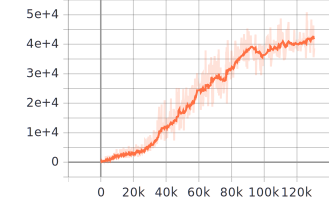
\includegraphics[width=0.3\textwidth,height=0.3\textwidth]{photo/appendix/atari_env/alien.png}
% 	}%
% 	\subfigure[Amidar-v4]{
% 		\centering
% 		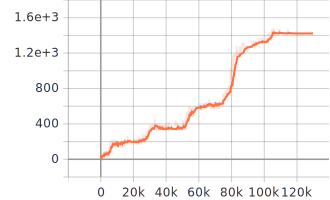
\includegraphics[width=0.3\textwidth,height=0.3\textwidth]{photo/appendix/atari_env/amidar.png}
% 	}%
% 	\subfigure[Assault-v4]{
% 		\centering
% 		\includegraphics[width=0.3\textwidth,height=0.3\textwidth]{photo/appendix/atari_env/Assault.png}
% 	}%
% 	\caption{雅达利游戏平台介绍图-1}
% 	\label{fig: ale 1}
% \end{figure}
% \vspace{-1.5cm}
% \begin{figure}[!ht]
% 	\centering
% 	\subfigure[Asterix-v4]{
% 		\centering
% 		\includegraphics[width=0.3\textwidth,height=0.3\textwidth]{photo/appendix/atari_env/Asterix.png}
% 	}%
% 	\subfigure[Asteroids-v4]{
% 		\centering
% 		\includegraphics[width=0.3\textwidth,height=0.3\textwidth]{photo/appendix/atari_env/Asteroids.png}
% 	}
% 	\subfigure[Atlantis-v4]{
% 		\centering
% 		\includegraphics[width=0.3\textwidth,height=0.3\textwidth]{photo/appendix/atari_env/Atlantis.png}
% 	}%
% 	\caption{雅达利游戏平台介绍图-2}
% 	\label{fig: ale 2}
% \end{figure}
% \vspace{-1.5cm}
% \begin{figure}[!ht]
% 	\centering
% 	\subfigure[BankHeist-v4]{
% 		\centering
% 		\includegraphics[width=0.3\textwidth,height=0.3\textwidth]{photo/appendix/atari_env/BankHeist.png}
% 	}%
% 	\subfigure[BattleZone-v4]{
% 		\centering
% 		\includegraphics[width=0.3\textwidth,height=0.3\textwidth]{photo/appendix/atari_env/BattleZone.png}
% 	}%
% 	\subfigure[BeamRider-v4]{
% 		\centering
% 		\includegraphics[width=0.3\textwidth,height=0.3\textwidth]{photo/appendix/atari_env/BeamRider.png}
% 	}%
% 	\caption{雅达利游戏平台介绍图-3}
% 	\label{fig: ale 3}
% \end{figure}
% \vspace{-1.5cm}

% \clearpage
% \vspace{-1.5cm}
% \begin{figure}[!ht]
% 	\centering
% 	\subfigure[Berzerk-v4]{
% 	\centering
% 	\includegraphics[width=0.3\textwidth,height=0.3\textwidth]{photo/appendix/atari_env/Berzerk.png}
%     }%
% 	\subfigure[Bowling-v4]{
% 		\centering
% 		\includegraphics[width=0.3\textwidth,height=0.3\textwidth]{photo/appendix/atari_env/Bowling.png}
% 	}%
% 	\subfigure[Boxing-v4]{
% 		\centering
% 		\includegraphics[width=0.3\textwidth,height=0.3\textwidth]{photo/appendix/atari_env/Boxing.png}
% 	}%
% 	\caption{雅达利游戏平台介绍图-4}
% 	\label{fig: ale 4}
% \end{figure}
% \vspace{-1.5cm}
% \begin{figure}[!ht]
% 	\centering
% 	\subfigure[Breakout-v4]{
% 		\centering
% 		\includegraphics[width=0.3\textwidth,height=0.3\textwidth]{photo/appendix/atari_env/Breakout.png}
% 	}%
% 	\subfigure[Centipede-v4]{
% 		\centering
% 		\includegraphics[width=0.3\textwidth,height=0.3\textwidth]{photo/appendix/atari_env/Centipede.png}
% 	}%
% 	\subfigure[ChopperCommand-v4]{
% 		\centering
% 		\includegraphics[width=0.3\textwidth,height=0.3\textwidth]{photo/appendix/atari_env/ChopperCommand.png}
% 	}%
% 	\caption{雅达利游戏平台介绍图-5}
% 	\label{fig: ale 5}
% \end{figure}
% \vspace{-1.5cm}
% \begin{figure}[!ht]
% 	\centering
% 	\subfigure[CrazyClimber-v4]{
% 		\centering
% 		\includegraphics[width=0.3\textwidth,height=0.3\textwidth]{photo/appendix/atari_env/Assault.png}
% 	}%
% 	\subfigure[Defender-v4]{
% 		\centering
% 		\includegraphics[width=0.3\textwidth,height=0.3\textwidth]{photo/appendix/atari_env/DemonAttack.png}
% 	}%
% 	\subfigure[DemonAttack-v4]{
% 		\centering
% 		\includegraphics[width=0.3\textwidth,height=0.3\textwidth]{photo/appendix/atari_env/DemonAttack.png}
% 	}%
% 	\caption{雅达利游戏平台介绍图-6}
% 	\label{fig: ale 6}
% \end{figure}
% \vspace{-1.5cm}

% \clearpage
% \vspace{-1.5cm}
% \begin{figure}[!ht]
% 	\centering
% 	\subfigure[DoubleDunk-v4]{
% 		\centering
% 		\includegraphics[width=0.3\textwidth,height=0.3\textwidth]{photo/appendix/atari_env/DoubleDunk.png}
% 	}%
% 	\subfigure[Enduro-v4]{
% 		\centering
% 		\includegraphics[width=0.3\textwidth,height=0.3\textwidth]{photo/appendix/atari_env/Enduro.png}
% 	}%
% 	\subfigure[FishingDerby-v4]{
% 		\centering
% 		\includegraphics[width=0.3\textwidth,height=0.3\textwidth]{photo/appendix/atari_env/FishingDerby.png}
% 	}%
% 	\caption{雅达利游戏平台介绍图-7}
% 	\label{fig: ale 7}
% \end{figure}
% \vspace{-1.5cm}
% \begin{figure}[!ht]
% 	\centering
% 	\subfigure[Freeway-v4]{
% 		\centering
% 		\includegraphics[width=0.3\textwidth,height=0.3\textwidth]{photo/appendix/atari_env/Freeway.png}
% 	}%
% 	\subfigure[Frostbite-v4]{
% 		\centering
% 		\includegraphics[width=0.3\textwidth,height=0.3\textwidth]{photo/appendix/atari_env/Frostbite.png}
% 	}%
% 	\subfigure[Gopher-v4]{
% 		\centering
% 		\includegraphics[width=0.3\textwidth,height=0.3\textwidth]{photo/appendix/atari_env/Gopher.png}
% 	}%
% 	\caption{雅达利游戏平台介绍图-8}
% 	\label{fig: ale 8}
% \end{figure}
% \vspace{-1.5cm}
% \begin{figure}[!ht]
% 	\centering
% 	\subfigure[Gravitar-v4]{
% 		\centering
% 		\includegraphics[width=0.3\textwidth,height=0.3\textwidth]{photo/appendix/atari_env/Gravitar.png}
% 	}%
% 	\subfigure[Hero-v4]{
% 		\centering
% 		\includegraphics[width=0.3\textwidth,height=0.3\textwidth]{photo/appendix/atari_env/HERO.png}
% 	}%
% 	\subfigure[IceHockey-v4]{
% 		\centering
% 		\includegraphics[width=0.3\textwidth,height=0.3\textwidth]{photo/appendix/atari_env/IceHockey.png}
% 	}%
% 	\caption{雅达利游戏平台介绍图-9}
% 	\label{fig: ale 9}
% \end{figure}
% \vspace{-1.5cm}

% \clearpage
% \vspace{-1.5cm}
% \begin{figure}[!ht]
% 	\centering
% 	\subfigure[Jamesbond-v4]{
% 		\centering
% 		\includegraphics[width=0.3\textwidth,height=0.3\textwidth]{photo/appendix/atari_env/Jamesbond.png}
% 	}%
% 	\subfigure[Kangaroo-v4]{
% 		\centering
% 		\includegraphics[width=0.3\textwidth,height=0.3\textwidth]{photo/appendix/atari_env/Kangaroo.png}
% 	}%
% 	\subfigure[Krull-v4]{
% 		\centering
% 		\includegraphics[width=0.3\textwidth,height=0.3\textwidth]{photo/appendix/atari_env/Krull.png}
% 	}%
% 	\caption{雅达利游戏平台介绍图-10}
% 	\label{fig: ale 10}
% \end{figure}
% \vspace{-1.5cm}
% \begin{figure}[!ht]
% 	\centering
% 	\subfigure[KungFuMaster-v4]{
% 		\centering
% 		\includegraphics[width=0.3\textwidth,height=0.3\textwidth]{photo/appendix/atari_env/KungFuMaster.png}
% 	}%
% 	\subfigure[MontezumaRevenge-v4]{
% 		\centering
% 		\includegraphics[width=0.3\textwidth,height=0.3\textwidth]{photo/appendix/atari_env/MontezumaRevenge.png}
% 	}%
% 	\subfigure[MsPacman-v4]{
% 		\centering
% 		\includegraphics[width=0.3\textwidth,height=0.3\textwidth]{photo/appendix/atari_env/MsPacman.png}
% 	}%
% 	\caption{雅达利游戏平台介绍图-11}
% 	\label{fig: ale 11}
% \end{figure}
% \vspace{-1.5cm}
% \begin{figure}[!ht]
% 	\centering
% 	\subfigure[NameThisGame-v4]{
% 		\centering
% 		\includegraphics[width=0.3\textwidth,height=0.3\textwidth]{photo/appendix/atari_env/NameThisGame.png}
% 	}%
% 	\subfigure[Phoenix-v4]{
% 		\centering
% 		\includegraphics[width=0.3\textwidth,height=0.3\textwidth]{photo/appendix/atari_env/Phoenix.png}
% 	}%
% 	\subfigure[Pitfall-v4]{
% 		\centering
% 		\includegraphics[width=0.3\textwidth,height=0.3\textwidth]{photo/appendix/atari_env/Pitfall.png}
% 	}%
% 	\caption{雅达利游戏平台介绍图-12}
% 	\label{fig: ale 12}
% \end{figure}
% \vspace{-1.5cm}

% \clearpage
% \vspace{-1.5cm}
% \begin{figure}[!ht]
% 	\centering
% 	\subfigure[Pong-v4]{
% 		\centering
% 		\includegraphics[width=0.3\textwidth,height=0.3\textwidth]{photo/appendix/atari_env/Pong.png}
% 	}%
% 	\subfigure[PrivateEye-v4]{
% 		\centering
% 		\includegraphics[width=0.3\textwidth,height=0.3\textwidth]{photo/appendix/atari_env/PrivateEye.png}
% 	}%
% 	\subfigure[Qbert-v4]{
% 		\centering
% 		\includegraphics[width=0.3\textwidth,height=0.3\textwidth]{photo/appendix/atari_env/Qbert.png}
% 	}%
% 	\caption{雅达利游戏平台介绍图-13}
% 	\label{fig: ale 13}
% \end{figure}
% \vspace{-1.5cm}
% \begin{figure}[!ht]
% 	\centering
% 	\subfigure[Riverraid-v4]{
% 		\centering
% 		\includegraphics[width=0.3\textwidth,height=0.3\textwidth]{photo/appendix/atari_env/Riverraid.png}
% 	}%
% 	\subfigure[RoadRunner-v4]{
% 		\centering
% 		\includegraphics[width=0.3\textwidth,height=0.3\textwidth]{photo/appendix/atari_env/RoadRunner.png}
% 	}%
% 	\subfigure[Robotank-v4]{
% 		\centering
% 		\includegraphics[width=0.3\textwidth,height=0.3\textwidth]{photo/appendix/atari_env/Robotank.png}
% 	}%
% 	\caption{雅达利游戏平台介绍图-14}
% 	\label{fig: ale 14}
% \end{figure}
% \vspace{-1.5cm}
% \begin{figure}[!ht]
% 	\centering
% 	\subfigure[Seaquest-v4]{
% 		\centering
% 		\includegraphics[width=0.3\textwidth,height=0.3\textwidth]{photo/appendix/atari_env/Seaquest.png}
% 	}%
% 	\subfigure[Skiing-v4]{
% 		\centering
% 		\includegraphics[width=0.3\textwidth,height=0.3\textwidth]{photo/appendix/atari_env/Skiing.png}
% 	}%
% 	\subfigure[Solaris-v4]{
% 		\centering
% 		\includegraphics[width=0.3\textwidth,height=0.3\textwidth]{photo/appendix/atari_env/Solaris.png}
% 	}%
% 	\caption{雅达利游戏平台介绍图-15}
% 	\label{fig: ale 15}
% \end{figure}
% \vspace{-1.5cm}

% \clearpage
% \vspace{-1.5cm}
% \begin{figure}[!ht]
% 	\centering
% 	\subfigure[SpaceInvaders-v4]{
% 		\centering
% 		\includegraphics[width=0.3\textwidth,height=0.3\textwidth]{photo/appendix/atari_env/SpaceInvaders.png}
% 	}%
% 	\subfigure[StarGunner-v4]{
% 		\centering
% 		\includegraphics[width=0.3\textwidth,height=0.3\textwidth]{photo/appendix/atari_env/StarGunner.png}
% 	}%
% 	\subfigure[Surround-v4]{
% 		\centering
% 		\includegraphics[width=0.3\textwidth,height=0.3\textwidth]{photo/appendix/atari_env/Surround.png}
% 	}
% 	\caption{雅达利游戏平台介绍图-16}
% 	\label{fig: ale 16}
% \end{figure}
% \vspace{-1.5cm}
% \begin{figure}[!ht]
% 	\centering
% 	\subfigure[Tennis-v4]{
% 		\centering
% 		\includegraphics[width=0.3\textwidth,height=0.3\textwidth]{photo/appendix/atari_env/Tennis.png}
% 	}%
% 	\subfigure[TimePilot-v4]{
% 		\centering
% 		\includegraphics[width=0.3\textwidth,height=0.3\textwidth]{photo/appendix/atari_env/TimePilot.png}
% 	}%
% 	\subfigure[Tutankham-v4]{
% 		\centering
% 		\includegraphics[width=0.3\textwidth,height=0.3\textwidth]{photo/appendix/atari_env/Tutankham.png}
% 	}%
% 	\caption{雅达利游戏平台介绍图-17}
% 	\label{fig: ale 17}
% \end{figure}
% \vspace{-1.5cm}
% \begin{figure}[!ht]
% 	\centering
% 	\subfigure[UpNDown-v4]{
% 		\centering
% 		\includegraphics[width=0.3\textwidth,height=0.3\textwidth]{photo/appendix/atari_env/UpNDown.png}
% 	}%
% 	\subfigure[Venture-v4]{
% 		\centering
% 		\includegraphics[width=0.3\textwidth,height=0.3\textwidth]{photo/appendix/atari_env/Venture.png}
% 	}%
% 	\subfigure[VideoPinball-v4]{
% 		\centering
% 		\includegraphics[width=0.3\textwidth,height=0.3\textwidth]{photo/appendix/atari_env/VideoPinball.png}
% 	}%
% 	\caption{雅达利游戏平台介绍图-18}
% 	\label{fig: ale 18}
% \end{figure}
% \vspace{-1.5cm}
% \clearpage
% \vspace{-1.5cm}
% \begin{figure}[!ht]
% 	\centering
% 	\subfigure[WizardOfWor-v4]{
% 		\centering
% 		\includegraphics[width=0.3\textwidth,height=0.3\textwidth]{photo/appendix/atari_env/WizardOfWor.png}
% 	}%
% 	\subfigure[YarsRevenge-v4]{
% 		\centering
% 		\includegraphics[width=0.3\textwidth,height=0.3\textwidth]{photo/appendix/atari_env/YarsRevenge.png}
% 	}%
% 	\subfigure[Zaxxon-v4]{
% 		\centering
% 		\includegraphics[width=0.3\textwidth,height=0.3\textwidth]{photo/appendix/atari_env/Zaxxon.png}
% 	}%
% 	\caption{雅达利游戏平台介绍图-19}
% 	\label{fig: ale 19}
% \end{figure}
% \clearpage


% \section{算法超参数}
% \label{sec: appendic hyperparameters}
% 这一节中我们展示我们算法的超参数,全部超参数如表\ref{tab:fixed_model_hyperparameters_atari}所示。
% \begin{center}
% \setlength{\tabcolsep}{1.0pt}
% \begin{table}[H]
% \caption{雅达利实验超参数设置}
% \begin{center}
% \begin{tabular}{c||c}
% \toprule
% \textbf{Parameter} & \textbf{Value}  \\
% \midrule
% 图片尺寸 & $84 \times 84$ \\
% 使用灰度图 & Yes \\
% 动作重复次数 & 4 \\
% 帧压缩次数 & 4 \\
% 动作空间 & 18 \\
% 丢失生命时是否结束轨迹 & No \\
% 样本量& 200M \\
% 并行环境量 & 32 \\
% 奖励变换 & $\log (abs (r) + 1.0) \cdot (2 \cdot 1_{\{r \geq 0\}} - 1_{\{r < 0\}})$ \\
% 切割奖励 & No \\
% 内生性奖励 & No \\
% 最小序列长 & 40 \\
% 序列长度 & 80 \\
% 自举估计 & Yes \\
% 批大小 & 64 \\
% $\gamma$ & 0.997 \\
% $V$ loss 系数 ($\xi$) & 1.0 \\
% $Q$ loss 系数 ($\alpha$) & 10.0 \\
% $\pi$ loss 系数 ($\beta$) & 10.0 \\
% 熵正则化 & No \\
% LSTM 单元& 256 \\
% 优化器 & Adam \\
% 学习率& 5e-4 \\
% 优化器参数$\beta_1$ & 0.9 \\
% 优化器参数 $\beta_2$ & 0.98 \\
% 优化器参数 $\epsilon$ & 1e-6 \\
% \bottomrule
% \end{tabular}
% \end{center}
% \label{tab:fixed_model_hyperparameters_atari}
% \end{table}
% \end{center}
% \clearpage

% \section{雅达利游戏训练曲线}
% \label{App: atari cruve}
% 本节中,我们主要给出我们算法在雅达利57个游戏上的实验得分曲线,来证明AlphaAtari算法的有效性。其主要分为19组图。即图\ref{fig: atari score 1}、图\ref{fig: atari score 2}、图\ref{fig: atari score 3}、图\ref{fig: atari score 4}、图\ref{fig: atari score 5}、图\ref{fig: atari score 6}、图\ref{fig: atari score 7}、图\ref{fig: atari score 8}、图\ref{fig: atari score 9}、图\ref{fig: atari score 10}、图\ref{fig: atari score 11}、图\ref{fig: atari score 12}、图\ref{fig: atari score 13}、图\ref{fig: atari score 14}、图\ref{fig: atari score 15}、图\ref{fig: atari score 16}、图\ref{fig: atari score 17}、图\ref{fig: atari score 18}、图\ref{fig: atari score 19}等。
% % \renewcommand{\thesubfigure}{\arabic{subfigure}.} % 数字编号
% % \setcounter{subfigure}{0}
% \begin{figure}[!ht]
%     \subfigure[alien]{
%     \includesvg[width=0.3\textwidth,inkscapelatex=false]{photo/appendix/atari_score/alien.svg}
%     }
%     \subfigure[amidar]{
%     \includesvg[width=0.3\textwidth,inkscapelatex=false]{photo/appendix/atari_score/amidar.svg}
%     }
%     \subfigure[assault]{
%     \includesvg[width=0.3\textwidth,inkscapelatex=false]{photo/appendix/atari_score/assault.svg}
%     }
%     \caption{实验效果评估图-1}
% 	\label{fig: atari score 1}
% \end{figure}

% \begin{figure}[!ht]
%     \subfigure[asterix]{
%     \includesvg[width=0.3\textwidth,inkscapelatex=false]{photo/appendix/atari_score/asterix.svg}
%     }
%     \subfigure[asteroids]{
%     \includesvg[width=0.3\textwidth,inkscapelatex=false]{photo/appendix/atari_score/asteroids.svg}
%     }
%     \subfigure[atlantis]{
%     \includesvg[width=0.3\textwidth,inkscapelatex=false]{photo/appendix/atari_score/atlantis.svg}
%     }
%         \caption{实验效果评估图-2}
% 	\label{fig: atari score 2}
% \end{figure}

% \begin{figure}[!ht]
%     \subfigure[bank\_heist]{
%     \includesvg[width=0.3\textwidth,inkscapelatex=false]{photo/appendix/atari_score/bank_heist.svg}
%     }
%     \subfigure[battle\_zone]{
%     \includesvg[width=0.3\textwidth,inkscapelatex=false]{photo/appendix/atari_score/battle_zone.svg}
%     }
%     \subfigure[beam\_rider]{
%     \includesvg[width=0.3\textwidth,inkscapelatex=false]{photo/appendix/atari_score/beam_rider.svg}
%     }
%         \caption{实验效果评估图-3}
% 	\label{fig: atari score 3}
% \end{figure}
% \begin{figure}[!ht]
%     \subfigure[berzerk]{
%     \includesvg[width=0.3\textwidth,inkscapelatex=false]{photo/appendix/atari_score/berzerk.svg}
%     }
%     \subfigure[bowling]{
%     \includesvg[width=0.3\textwidth,inkscapelatex=false]{photo/appendix/atari_score/bowling.svg}
%     }
%     \subfigure[boxing]{
%     \includesvg[width=0.3\textwidth,inkscapelatex=false]{photo/appendix/atari_score/boxing.svg}
%     }
%         \caption{实验效果评估图-4}
%     \label{fig: atari score 4}
% \end{figure}

% \begin{figure}[!ht]
%     \subfigure[breakout]{
%     \includesvg[width=0.3\textwidth,inkscapelatex=false]{photo/appendix/atari_score/breakout.svg}
%     }
%     \subfigure[centipede]{
%     \includesvg[width=0.3\textwidth,inkscapelatex=false]{photo/appendix/atari_score/centipede.svg}
%     }
%     \subfigure[chopper\_command]{
%     \includesvg[width=0.3\textwidth,inkscapelatex=false]{photo/appendix/atari_score/chopper_command.svg}
%     }
%         \caption{实验效果评估图-5}
% 	\label{fig: atari score 5}
% \end{figure}

% \begin{figure}[!ht]
%     \subfigure[crazy\_climber]{
%     \includesvg[width=0.3\textwidth,inkscapelatex=false]{photo/appendix/atari_score/crazy_climber.svg}
%     }
%     \subfigure[defender]{
%     \includesvg[width=0.3\textwidth,inkscapelatex=false]{photo/appendix/atari_score/defender.svg}
%     }
%     \subfigure[demon\_attack]{
%     \includesvg[width=0.3\textwidth,inkscapelatex=false]{photo/appendix/atari_score/demon_attack.svg}
%     }
%         \caption{实验效果评估图-6}
% 	\label{fig: atari score 6}
% \end{figure}
% \begin{figure}[!ht]
%     \subfigure[double\_dunk]{
%     \includesvg[width=0.3\textwidth,inkscapelatex=false]{photo/appendix/atari_score/double_dunk.svg}
%     }
%     \subfigure[enduro]{
%     \includesvg[width=0.3\textwidth,inkscapelatex=false]{photo/appendix/atari_score/enduro.svg}
%     }
%     \subfigure[fishing\_derby]{
%     \includesvg[width=0.3\textwidth,inkscapelatex=false]{photo/appendix/atari_score/fishing_derby.svg}
%     }
%         \caption{实验效果评估图-7}
% 	\label{fig: atari score 7}
% \end{figure}

% \begin{figure}[!ht]
%     \subfigure[freeway]{
%     \includesvg[width=0.3\textwidth,inkscapelatex=false]{photo/appendix/atari_score/freeway.svg}
%     }
%     \subfigure[frostbite]{
%     \includesvg[width=0.3\textwidth,inkscapelatex=false]{photo/appendix/atari_score/frostbite.svg}
%     }
%     \subfigure[gopher]{
%     \includesvg[width=0.3\textwidth,inkscapelatex=false]{photo/appendix/atari_score/gopher.svg}
%     }
%         \caption{实验效果评估图-8}
% 	\label{fig: atari score 8}
% \end{figure}

% \begin{figure}[!ht]
%     \subfigure[gravitar]{
%     \includesvg[width=0.3\textwidth,inkscapelatex=false]{photo/appendix/atari_score/gravitar.svg}
%     }
%     \subfigure[hero]{
%     \includesvg[width=0.3\textwidth,inkscapelatex=false]{photo/appendix/atari_score/hero.svg}
%     }
%     \subfigure[ice\_hockey]{
%     \includesvg[width=0.3\textwidth,inkscapelatex=false]{photo/appendix/atari_score/ice_hockey.svg}
%     }
%         \caption{实验效果评估图-9}
% 	\label{fig: atari score 9}
% \end{figure}
% \begin{figure}[!ht]
%     \subfigure[jamesbond]{
%         \includesvg[width=0.3\textwidth,inkscapelatex=false]{photo/appendix/atari_score/jamesbond.svg}
%         }
%     \subfigure[kangaroo]{
%     \includesvg[width=0.3\textwidth,inkscapelatex=false]{photo/appendix/atari_score/kangaroo.svg}
%     }
%     \subfigure[krull]{
%     \includesvg[width=0.3\textwidth,inkscapelatex=false]{photo/appendix/atari_score/krull.svg}
%     }
%         \caption{实验效果评估图-10}
% 	\label{fig: atari score 10}
% \end{figure}

% \begin{figure}[!ht]
% \subfigure[kung\_fu\_master]{
%     \includesvg[width=0.3\textwidth,inkscapelatex=false]{photo/appendix/atari_score/kung_fu_master.svg}
%     }
%     \subfigure[montezuma\_revenge]{
%     \includesvg[width=0.3\textwidth,inkscapelatex=false]{photo/appendix/atari_score/montezuma_revenge.svg}
%     }
%     \subfigure[ms\_pacman]{
%     \includesvg[width=0.3\textwidth,inkscapelatex=false]{photo/appendix/atari_score/ms_pacman.svg}
%     }
%      \caption{实验效果评估图-11}
% 	\label{fig: atari score 11}
% \end{figure}

% \begin{figure}[!ht]
%  \subfigure[name\_this\_game]{
%     \includesvg[width=0.3\textwidth,inkscapelatex=false]{photo/appendix/atari_score/name_this_game.svg}
%     }
%     \subfigure[phoenix]{
%     \includesvg[width=0.3\textwidth,inkscapelatex=false]{photo/appendix/atari_score/phoenix.svg}
%     }
%     \subfigure[pitfall]{
%     \includesvg[width=0.3\textwidth,inkscapelatex=false]{photo/appendix/atari_score/pitfall.svg}
%     }
%         \caption{实验效果评估图-12}
% 	\label{fig: atari score 12}
% \end{figure}
% \begin{figure}[!ht]
% \subfigure[pong]{
%     \includesvg[width=0.3\textwidth,inkscapelatex=false]{photo/appendix/atari_score/pong.svg}
%     }
%     \subfigure[private\_eye]{
%     \includesvg[width=0.3\textwidth,inkscapelatex=false]{photo/appendix/atari_score/private_eye.svg}
%     }
%     \subfigure[qbert]{
%     \includesvg[width=0.3\textwidth,inkscapelatex=false]{photo/appendix/atari_score/qbert.svg}
%     }
%         \caption{实验效果评估图-13}
% 	\label{fig: atari score 13}
% \end{figure}

% \begin{figure}[!ht]
% \subfigure[riverraid]{
%     \includesvg[width=0.3\textwidth,inkscapelatex=false]{photo/appendix/atari_score/riverraid.svg}
%     }
%     \subfigure[road\_runner]{
%     \includesvg[width=0.3\textwidth,inkscapelatex=false]{photo/appendix/atari_score/road_runner.svg}
%     }
%     \subfigure[robotank]{
%     \includesvg[width=0.3\textwidth,inkscapelatex=false]{photo/appendix/atari_score/robotank.svg}
%     }
%         \caption{实验效果评估图-14}
% 	\label{fig: atari score 14}
% \end{figure}

% \begin{figure}[!ht]
%     \subfigure[seaquest]{
%     \includesvg[width=0.3\textwidth,inkscapelatex=false]{photo/appendix/atari_score/seaquest.svg}
%     }
%     \subfigure[skiing]{
%     \includesvg[width=0.3\textwidth,inkscapelatex=false]{photo/appendix/atari_score/skiing.svg}
%     }
%     \subfigure[solaris]{
%     \includesvg[width=0.3\textwidth,inkscapelatex=false]{photo/appendix/atari_score/solaris.svg}
%     }
%         \caption{实验效果评估图-15}
% 	\label{fig: atari score 15}
% \end{figure}
% \begin{figure}[!ht]
% \subfigure[space\_invader]{
%     \includesvg[width=0.3\textwidth,inkscapelatex=false]{photo/appendix/atari_score/space_invader.svg}
%     }
%     \subfigure[star\_gunner]{
%     \includesvg[width=0.3\textwidth,inkscapelatex=false]{photo/appendix/atari_score/star_gunner.svg}
%     }
%     \subfigure[surround]{
%     \includesvg[width=0.3\textwidth,inkscapelatex=false]{photo/appendix/atari_score/surround.svg}
%     }
%         \caption{实验效果评估图-16}
% 	\label{fig: atari score 16}
% \end{figure}

% \begin{figure}[!ht]
%  \subfigure[tennis]{
%     \includesvg[width=0.3\textwidth,inkscapelatex=false]{photo/appendix/atari_score/tennis.svg}
%     }
%     \subfigure[time\_pilot]{
%     \includesvg[width=0.3\textwidth,inkscapelatex=false]{photo/appendix/atari_score/time_pilot.svg}
%     }
%     \subfigure[tutankham]{
%     \includesvg[width=0.3\textwidth,inkscapelatex=false]{photo/appendix/atari_score/tutankham.svg}
%     }
%         \caption{实验效果评估图-17}
% 	\label{fig: atari score 17}
% \end{figure}

% \begin{figure}[!ht]
% \subfigure[up\_n\_down]{
%     \includesvg[width=0.3\textwidth,inkscapelatex=false]{photo/appendix/atari_score/up_n_down.svg}
%     }
%     \subfigure[venture]{
%     \includesvg[width=0.3\textwidth,inkscapelatex=false]{photo/appendix/atari_score/venture.svg}
%     }
%     \subfigure[video\_pinball]{
%     \includesvg[width=0.3\textwidth,inkscapelatex=false]{photo/appendix/atari_score/video_pinball.svg}
%     }
%         \caption{实验效果评估图-18}
% 	\label{fig: atari score 18}
% \end{figure}

% \begin{figure}[!ht]
%  \subfigure[wizard\_of\_wor]{
%     \includesvg[width=0.3\textwidth,inkscapelatex=false]{photo/appendix/atari_score/wizard_of_wor.svg}
%     }
%     \subfigure[yars\_revenge]{
%     \includesvg[width=0.3\textwidth,inkscapelatex=false]{photo/appendix/atari_score/yars_revenge.svg}
%     }
%     \subfigure[zaxxon]{
%     \includesvg[width=0.3\textwidth,inkscapelatex=false]{photo/appendix/atari_score/zaxxon.svg}
%     }
%         \caption{实验效果评估图-19}
% 	\label{fig: atari score 19}
% \end{figure}

% \clearpage

% \section{人类基准的雅达利游戏得分}
% \label{sec: appendix atari_score}
% 本小节中我们将分三个小节汇报所有算法以人类平均分数为基准的雅达利游戏得分。首先我们在表\ref{tab: 200M atari hns}中汇报200M训练量的算法,然后我们在表\ref{tab: 10B atari hns}中汇报10B+训练量算法的雅达利游戏得分,再然后我们在表\ref{tab: MBRL atari hns}中汇报基于模型的强化学习算法的雅达利游戏得分,最后我们在表\ref{tab: other atari hns}中汇报其他世界一流算法的游戏得分,通过本节的比较可以看出我们的算法AlphaAtari的性能超越世界一流算法,进一步验证了我们算法的有效性。下面我们逐个介绍算法的数据来源:

% \begin{enumerate}
%     \item 随机组分数来自于 \upcite{agent57}。
%     \item Rainbow的分数来自于 \upcite{rainbow}。
%     \item IMPALA的分数来自于 \upcite{impala}。
%     \item LASER的分数来自于 \upcite{laser}。
%     \item R2D2的分数来自于 \upcite{r2d2}。
%     \item NGU的分数来自于 \upcite{ngu}。
%     \item Agent57的分数来自于 \upcite{agent57}。
%     \item MuZero的分数来自于 \upcite{muzero}。
%     \item DreamerV2的分数来自于 \upcite{dreamerv2}。
%     \item SimPLe的分数来自于 \upcite{modelbasedatari}。
%     \item  Muesil的分数来自于 \upcite{muesli}。
% \end{enumerate}

% \begin{table}
% \caption{与200M算法相比分数对照表-基于人类基础得分}
% \label{tab: 200M atari hns}
% \begin{center}
% \scriptsize
% \setlength{\tabcolsep}{1.0pt}
% \begin{tabular}{|c|c|c|c c|c c|c c|c c|}
% \toprule
% Games & RND & HUMAN & RAINBOW & HNS(\%) & IMPALA & HNS(\%) & LASER & HNS(\%) & AlphaAtari & HNS(\%) \\
% \midrule
% Scale  &     &       & 200M   &       &  200M    &        & 200M   &
%       &  200M   &  \\
% \midrule
%  alien  & 227.8 & 7127.8            & 9491.7 & 134.26 & 15962.1  & 228.03 & 35565.9 & 512.15                        &\best{43384}      &\best{625.45}     \\
%  amidar & 5.8   & 1719.5            & \textbf{5131.2} & \textbf{299.08} & 1554.79  & 90.39  & 1829.2  & 106.4       &1442              &83.81             \\
%  assault & 222.4 & 742              & 14198.5 & 2689.78 & 19148.47 & 3642.43  & 21560.4 & 4106.62                   &\best{63876}      &\best{12250.50}  \\
%  asterix & 210   & 8503.3           & 428200 & 5160.67 & 300732   & 3623.67  & 240090  & 2892.46                    &\best{759910}     &\best{9160.41}   \\
%  asteroids & 719 & 47388.7          & 2712.8 & 4.27   & 108590.05 & 231.14  & 213025  &  454.91                     &\best{751970}     &\best{1609.72}   \\
%  atlantis & 12850 & 29028.1         & 826660 & 5030.32 & 849967.5 & 5174.39 & 841200 & 5120.19                      &\best{3803000}    &\best{23427.66}  \\
%  bank heist & 14.2 & 753.1          & 1358   & 181.86  & 1223.15  & 163.61  & 569.4  & 75.14                        &\best{1401}       &\best{187.68}     \\
%  battle zone & 236 & 37187.5        & 62010 & 167.18  & 20885    & 55.88  & 64953.3 & 175.14                        &\best{478830}     &\best{1295.20}   \\
%  beam rider & 363.9 & 16926.5       & 16850.2 & 99.54 & 32463.47 & 193.81 & 90881.6 & 546.52                        &\best{162100}     &\best{976.51}     \\
%  berzerk & 123.7 & 2630.4           & 2545.6   & 96.62  & 1852.7   & 68.98  & \textbf{25579.5} & \textbf{1015.51}   &7607              &298.53            \\
%  bowling & 23.1 & 160.7             & 30   & 5.01        & 59.92    & 26.76  & 48.3    & 18.31                      &\best{201.9}      &\best{129.94}     \\
%  boxing  & 0.1  & 12.1              & 99.6 & 829.17      & 99.96    & 832.17 & \textbf{100} & \textbf{832.5}        &\best{100}        &\best{832.50}     \\
%  breakout & 1.7 & 30.5              & 417.5 & 1443.75    & 787.34   & 2727.92 & 747.9 & 2590.97                     &\best{864}        &\best{2994.10}   \\
%  centipede & 2090.9 & 12017         & 8167.3 & 61.22   & 11049.75 & 90.26   & \textbf{292792} & \textbf{2928.65}    &155830            &1548.84          \\
%  chopper command & 811 & 7387.8     & 16654 & 240.89 & 28255  & 417.29  & 761699 & 11569.27                         &\best{999999}     &\best{15192.62}  \\
%  crazy climber & 10780.5 & 36829.4  & 168788.5 & 630.80 & 136950 & 503.69 & 167820  & 626.93                        &\best{201000}     &\best{759.39}     \\
%  defender & 2874.5 & 18688.9        & 55105 & 330.27 & 185203 & 1152.93 & 336953  & 2112.50                         &\best{893110}     &\best{5629.27}   \\
%  demon attack & 152.1 & 1971        & 111185 & 6104.40 & 132826.98 & 7294.24 & 133530 & 7332.89                     &\best{675530}     &\best{37131.12}  \\
%  double dunk & -18.6 & -16.4        & -0.3   & 831.82  & -0.33     & 830.45  & 14     & 1481.82                     &\best{24}         &\best{1936.36}    \\
%  enduro      & 0   & 860.5          & 2125.9 & 247.05  & 0       & 0.00     & 0    & 0.00                           &\best{14330}      &\best{1665.31 }  \\
%  fishing derby & -91.7 & -38.8      & 31.3 & 232.51  & 44.85   & 258.13    & 45.2   & 258.79                        &\best{59}         &\best{285.71   }  \\
%  freeway       & 0     & 29.6       & \textbf{34} & \textbf{114.86}  & 0     & 0.00       & 0    & 0.00             &\best{34}         &\best{114.86   }  \\
%  frostbite     & 65.2  & 4334.7     & 9590.5 & 223.10 & 317.75 & 5.92     & 5083.5 & 117.54                         &\best{10485}      &\best{244.05   }  \\
%  gopher  & 257.6 & 2412.5           & 70354.6 & 3252.91    & 66782.3 & 3087.14 & 114820.7 & 5316.40                 &\best{488830}     &\best{22672.63}  \\
%  gravitar & 173 & 3351.4            & 1419.3  & 39.21   & 359.5      & 5.87    & 1106.2   & 29.36                   &\best{5905}       &\best{180.34   }  \\
%  hero   & 1027 & 30826.4            & \textbf{55887.4} & \textbf{184.10}   & 33730.55  & 109.75  & 31628.7 & 102.69 &38330             &125.18            \\
%  ice hockey & -11.2 & 0.9           & 1.1    & 101.65   & 3.48      & 121.32   & 17.4    & 236.36                   &\best{44.94 }     &\best{463.97    } \\
%  jamesbond  & 29    & 302.8         & 19809 & 72.24   & 601.5     & 209.09   & 37999.8 & 13868.08                   &\best{594500}     &\best{217118.70} \\
%  kangaroo   & 52    & 3035          & \textbf{14637.5} & \textbf{488.05} & 1632    & 52.97    & 14308   & 477.91    &14500             &484.34            \\
%  krull     & 1598   & 2665.5        & 8741.5  & 669.18 & 8147.4  & 613.53   & 9387.5  &  729.70                     &\best{97575}      &\best{8990.82}   \\
%  kung fu master & 258.5 & 22736.3   & 52181 & 230.99 & 43375.5 & 191.82 & \textbf{607443} & \textbf{2701.26}        &140440            &623.64            \\
%  montezuma revenge&0&\textbf{4753.3}& 384   & 8.08   & 0       & 0.00   & 0.3    & 0.01                             &3000              &63.11             \\
%  ms pacman  & 307.3 & 6951.6        & 5380.4  & 76.35   & 7342.32 & 105.88 & 6565.5   & 94.19                       &\best{11536 }     &\best{169.00}     \\
%  name this game & 2292.3 & 8049     & 13136 & 188.37   & 21537.2 & 334.30 & 26219.5 & 415.64                        &\best{34434 }     &\best{558.34}     \\
%  phoenix & 761.5 & 7242.6  & 108529 & 1662.80   & 210996.45  & 3243.82 & 519304 & 8000.84                           &\best{894460}     &\best{13789.30}  \\
%  pitfall & -229.4 & \textbf{6463.7} & 0      & 3.43      & -1.66      & 3.40    & -0.6   & 3.42                     &0      &3.43       \\
%  pong    & -20.7  & 14.6   & 20.9   & 117.85    & 20.98      & 118.07  & \textbf{21}     &  \textbf{118.13}         &\best{21   }      &\best{118.13}     \\
%  private eye & 24.9&\textbf{69571.3}& 4234 & 6.05     & 98.5       & 0.11    & 96.3   & 0.10                        &15100      &21.68     \\
%  qbert  & 163.9 & 13455.0 & 33817.5 & 253.20   & \textbf{351200.12}  & \textbf{2641.14} & 21449.6 & 160.15          &27800             &207.93            \\
%  riverraid & 1338.5 & 17118.0       & 22920.8 & 136.77 & 29608.05  & 179.15  & \textbf{40362.7} & \textbf{247.31}   &28075             &169.44            \\
%  road runner & 11.5 & 7845          & 62041   & 791.85 & 57121     & 729.04  & 45289   & 578.00                     &\best{878600 }    &\best{11215.78}  \\
%  robotank   & 2.2   & 11.9          & 61.4   & 610.31    & 12.96     & 110.93  & 62.1    & 617.53                   &\best{108.2  }    &\best{1092.78 }  \\
%  seaquest  & 68.4 & 42054.7         & 15898.9 & 37.70    & 1753.2    & 4.01    & 2890.3  & 6.72                     &\best{1000000}    &\best{2381.57 }  \\
%  skiing & -17098  & \textbf{-4336.9}& -12957.8 & 32.44  & -10180.38 & 54.21   & -29968.4 & -100.86                  &-6774             &80.90             \\
%  solaris & 1236.3 & \textbf{12326.7}& 3560.3  & 20.96  & 2365      & 10.18   & 2273.5   & 9.35                      &11074             &88.70             \\
%  space invaders & 148 & 1668.7      & 18789 & 1225.82 & 43595.78 & 2857.09 & 51037.4 & 3346.45                      &\best{140460 }    &\best{9226.80}   \\
%  star gunner & 664 & 10250          & 127029    & 1318.22 & 200625   & 2085.97 & 321528  & 3347.21                  &\best{465750 }    &\best{4851.72}   \\
%  surround    & -10 & 6.5            & \textbf{9.7}       & \textbf{119.39}  & 7.56     & 106.42  & 8.4     & 111.52 &-7.8              &13.33             \\
%  tennis  & -23.8   & -8.3           & 0        & 153.55    & 0.55     & 157.10  & 12.2    & 232.26                  &\best{24       }  &\best{308.39   }  \\
%  time pilot & 3568 & 5229.2         & 12926 & 563.36     & 48481.5  & 2703.84 & 105316  & 6125.34                   &\best{216770}     &\best{12834.99}  \\
%  tutankham  & 11.4 & 167.6          & 241   & 146.99     & 292.11   & 179.71  & 278.9   & 171.25                    &\best{423.9 }     &\best{264.08   }  \\
%  up n down  & 533.4 & 11693.2       & 125755 & 1122.08 & 332546.75 & 2975.08 & 345727 & 3093.19                     &\best{986440}     &\best{8834.45 }  \\
%  venture    & 0     & 1187.5        & 5.5    & 0.46    & 0         & 0.00    & 0      & 0.00                        &\best{2035     }  &\best{171.37   }  \\
%  video pinball & 0 & 17667.9        & 533936.5 & 3022.07 & 572898.27 & 3242.59 & 511835 & 2896.98                   &\best{925830}     &\best{5240.18 }  \\
%  wizard of wor & 563.5 & 4756.5     & 17862.5 & 412.57 & 9157.5    & 204.96  & 29059.3 & 679.60                     &\best{64239 }     &\best{1519.90 }  \\
%  yars revenge & 3092.9 & 54576.9    & 102557 & 193.19 & 84231.14  & 157.60 & 166292.3  & 316.99                     &\best{972000}     &\best{1881.96 }  \\
%  zaxxon       & 32.5   & 9173.3     & 22209.5 & 242.62 & 32935.5   & 359.96 & 41118    & 449.47                     &\best{109140}     &\best{1193.63 }  \\
% \hline
% MEAN HNS(\%) &     0.00 & 100.00   &         & 873.97 &         & 957.34  &        & 1741.36 &      & \textbf{7812.98} \\
% \hline
% MEDIAN HNS(\%) & 0.00   & 100.00   &         & 230.99 &         & 191.82  &        & 454.91  &      & \textbf{832.50} \\
% \bottomrule
% \end{tabular}
% \end{center}
% \end{table}

% \clearpage

% \begin{table}
% \caption{与10B+算法相比分数对照表-基于人类基础得分}
% \label{tab: 10B atari hns}
% \begin{center}
% \scriptsize
% \setlength{\tabcolsep}{1.0pt}
% \begin{tabular}{|c|c c|c c|c c|c c|}
% \toprule
%  Games & R2D2 & HNS(\%) & NGU & HNS(\%) & AGENT57 & HNS(\%) & AlphaAtari & HNS(\%) \\
% \midrule
% Scale  & 10B   &        & 35B &         & 100B     &        & 200M & \\
% \midrule
%  alien  & 109038.4 & 1576.97 & 248100 & 3592.35 & \textbf{297638.17} & \textbf{4310.30}             &43384             &625.45                \\
%  amidar & 27751.24 & 1619.04 & 17800  & 1038.35 & \textbf{29660.08}  & \textbf{1730.42}             &1442              &83.81                 \\
%  assault & \textbf{90526.44} & \textbf{17379.53} & 34800 & 6654.66 & 67212.67 & 12892.66            &63876             &12250.50             \\
%  asterix & \textbf{999080}   & \textbf{12044.30} & 950700 & 11460.94 & 991384.42 & 11951.51         &759910            &9160.41              \\
%  asteroids & 265861.2 & 568.12 & 230500 & 492.36   & 150854.61 & 321.70                             &\best{751970}     &\best{1609.72}       \\
%  atlantis & 1576068   & 9662.56 & 1653600 & 10141.80 & 1528841.76 & 9370.64                         &\best{3803000}    &\best{23427.66}      \\
%  bank heist & \textbf{46285.6} & \textbf{6262.20} & 17400   & 2352.93  & 23071.5& 3120.49           &1401              &187.68                \\
%  battle zone & 513360 & 1388.64 & 691700  & 1871.27  & \textbf{934134.88}& \textbf{2527.36}         &478830            &1295.20              \\
%  beam rider & 128236.08 & 772.05 & 63600  & 381.80   & \textbf{300509.8} & \textbf{1812.19}         &162100            &976.51                \\
%  berzerk & 34134.8      & 1356.81 & 36200 & 1439.19  & \textbf{61507.83} & \textbf{2448.80}         &7607              &298.53                \\
%  bowling & 196.36       & 125.92  & 211.9 & 137.21   & \textbf{251.18}   & \textbf{165.76}          &201.9             &129.94                \\
%  boxing  & 99.16        & 825.50  & 99.7  & 830.00   & \textbf{100}      & \textbf{832.50}          &\best{100}        &\best{832.50}         \\
%  breakout & 795.36      & 2755.76 & 559.2 & 1935.76  & 790.4 & 2738.54                  &\best{864}        &\best{2994.10}       \\
%  centipede & 532921.84  & 5347.83 & \textbf{577800} & \textbf{5799.95} & 412847.86& 4138.15         &155830            &1548.84              \\
%  chopper command&960648&14594.29&999900&15191.11&999900&15191.11                                    &\best{999999}&\best{15192.62}      \\
%  crazy climber & 312768   & 1205.59  & 313400 & 1208.11&\textbf{565909.85}&\textbf{2216.18}         &201000            &759.39                \\
%  defender & 562106        & 3536.22  & 664100 & 4181.16  & 677642.78 & 4266.80                      &\best{893110}     &\best{5629.27 }      \\
%  demon attack & 143664.6  & 7890.07  & 143500 & 7881.02  & 143161.44 & 7862.41                      &\best{675530}     &\best{37131.12}      \\
%  double dunk & 23.12      & 1896.36  & -14.1  & 204.55   & 23.93& 1933.18         &\textbf{24}             &\textbf{1936.36}              \\
%  enduro      & 2376.68    & 276.20   & 2000   & 232.42   & 2367.71   & 275.16                       &\best{14330}      &\best{1665.31}       \\
%  fishing derby & 81.96    & 328.28   & 32     & 233.84   & \textbf{86.97}& \textbf{337.75}          &59                &285.71                \\
%  freeway       & \textbf{34}       & \textbf{114.86}   & 28.5   & 96.28    & 32.59& 110.10          &\best{34}         &\best{114.86}         \\
%  frostbite    & 11238.4  & 261.70   & 206400 & 4832.76&\textbf{541280.88}&\textbf{12676.32}         &10485             &244.05                \\
%  gopher  & 122196        & 5658.66  & 113400 & 5250.47  & 117777.08 & 5453.59                       &\best{488830}     &\best{22672.63}      \\
%  gravitar & 6750         & 206.93   & 14200  & 441/32  &\textbf{19213.96}&\textbf{599.07}           &5905              &180.34                \\
%  hero   & 37030.4        & 120.82   & 69400  & 229.44&\textbf{114736.26}&\textbf{381.58}            &38330             &125.18                \\
%  ice hockey & \textbf{71.56}      & \textbf{683.97}   &-4.1   & 58.68    & 63.64& 618.51            &44.94             &463.97                \\
%  jamesbond  & 23266      & 8486.85  & 26600  & 9704.53  & 135784.96 & 49582.16                      &\best{594500}     &\best{217118.70}     \\
%  kangaroo   & 14112      & 471.34   & \textbf{35100}  & \textbf{1174.92}&24034.16& 803.96           &14500             &484.34                \\
%  krull     & 145284.8    & 13460.12 & 127400&11784.73& \textbf{251997.31}&\textbf{23456.61}         &97575             &8990.82              \\
%  kung fu master & 200176 & 889.40   & \textbf{212100} & \textbf{942.45}   & 206845.82 & 919.07      &140440            &623.64                \\
%  montezuma revenge & 2504 & 52.68   & \textbf{10400}  & \textbf{218.80} &9352.01& 196.75            &3000              &63.11                 \\
%  ms pacman  & 29928.2     & 445.81  & 40800  & 609.44& \textbf{63994.44}&\textbf{958.52}            &11536             &169.00                \\
%  name this game & 45214.8 & 745.61  & 23900  & 375.35&\textbf{54386.77}&\textbf{904.94}             &34434             &558.34                \\
%  phoenix & 811621.6       & 125.11  & \textbf{959100} &\textbf{14786.66}&908264.15&14002.29         &894460            &13789.30             \\
%  pitfall & 0              & 3.43    & 7800   & 119.97&\textbf{18756.01}&\textbf{283.66}             &0                 &3.43                  \\
%  pong    & \textbf{21}             & \textbf{118.13}  & 19.6   & 114.16   & 20.67& 117.20           &\best{21}         &\best{118.13}         \\
%  private eye & 300        & 0.40    & \textbf{100000} & \textbf{143.75}& 79716.46&114.59            &15100             &21.68                 \\
%  qbert  & 161000          & 1210.10 & 451900 & 3398.79&\textbf{580328.14}&\textbf{4365.06}          &27800             &207.93                \\
%  riverraid & 34076.4      & 207.47  & 36700  & 224.10 & \textbf{63318.67}&\textbf{392.79}           &28075             &169.44                \\
%  road runner & 498660     & 6365.59 & 128600 & 1641.52  & 243025.8&3102.24                          &\best{878600}     &\best{11215.78}      \\
%  robotank   & \textbf{132.4}       & \textbf{1342.27} & 9.1    & 71.13 &127.32 &1289.90             &108.2             &1092.78              \\
%  seaquest  & 999991.84    & 2381.55 & \textbf{1000000} & \textbf{2381.57}&999997.63&2381.56         &\best{1000000}    &\best{2381.57}       \\
%  skiing & -29970.32       & -100.87 & -22977.9 & -46.08 & \textbf{-4202.6}  &\textbf{101.05}        &-6774             &80.90                 \\
%  solaris & 4198.4         & 26.71   & 4700     & 31.23  & \textbf{44199.93}& \textbf{387.39}        &11074             &88.70                 \\
%  space invaders & 55889   & 3665.48 & 43400    & 2844.22 & 48680.86 & 3191.48                       &\best{140460}     &9226.80              \\
%  star gunner & 521728     & 5435.68 & 414600   &4318.13&\textbf{839573.53}&\textbf{8751.40}         &465750            &4851.72              \\
%  surround    & \textbf{9.96}       & \textbf{120.97}  & -9.6     & 2.42    & 9.5&118.18             &-7.8              &13.33                 \\
%  tennis  & \textbf{24}             & \textbf{308.39}  & 10.2     & 219.35 & 23.84& 307.35           &\best{24}                &\best{308.39}                \\
%  time pilot & 348932    & 20791.28 & 344700 & 20536.51&\textbf{405425.31}&\textbf{24192.24}         &216770            &12834.99             \\
%  tutankham  & 393.64    & 244.71   & 191.1   & 115.04   & \textbf{2354.91}&\textbf{1500.33}         &423.9             &264.08                \\
%  up n down  & 542918.8  & 4860.17  & 620100  & 5551.77  & 623805.73 & 5584.98                       &\best{986440}     &\best{8834.45}       \\
%  venture    & 1992      & 167.75   & 1700    & 143.16   &\textbf{2623.71}  &\textbf{220.94}         &2035              &171.37                \\
%  video pinball & 483569.72 & 2737.00 & 965300 & 5463.58 &\textbf{992340.74}&\textbf{5616.63}        &925830            &5240.18              \\
%  wizard of wor & 133264 & 3164.81  & 106200  & 2519.35  &\textbf{157306.41}&\textbf{3738.20}        &64293             &1519.90              \\
%  yars revenge & 918854.32 & 1778.73 & 986000 & 1909.15  &\textbf{998532.37}&\textbf{1933.49}        &972000            &1881.96              \\
%  zaxxon & 181372        & 1983.85  & 111100  & 1215.07  &\textbf{249808.9} &\textbf{2732.54}        &109140            &1193.63              \\
% \hline
% MEAN HNS(\%) &               & 3374.31  &         &  3169.90 &           & 4763.69  &     & \best{7812.98} \\
% \hline
% MEDIAN HNS(\%) &            & 1342.27   &         & 1208.11  &           & \textbf{1933.49}  &     & 832.50 \\
% \bottomrule
% \end{tabular}
% % \caption{与10B+算法相比分数对照表}
% \end{center}
% \end{table}
% \clearpage


% \begin{table}
% \caption{与基于模型算法相比分数对照表-基于人类基础得分}
% \label{tab: MBRL atari hns}
% \begin{center}
% \scriptsize
% \setlength{\tabcolsep}{1.0pt}
% \begin{tabular}{|c|c c|c c|c c|c c|}
% \toprule
%  Games              & MuZero         & HNS(\%)      & DreamerV2 & HNS(\%)    & SimPLe             & HNS(\%)          & AlphaAtari     & HNS(\%) \\
% \midrule
% Scale               & 20B            &              & 200M      &            & 1M               &                  & 200M     & \\
% \midrule    
%  alien              & \textbf{741812.63}      & \textbf{10747.61}     &3483       & 47.18      &616.9     & 5.64    & 43384       & 625.45    \\
%  amidar             & \textbf{28634.39 }      & \textbf{1670.57    }  &2028       & 118.00     &74.3      & 4.00    & 1442        & 83.81     \\
%  assault            & \textbf{143972.03}      & \textbf{27665.44}     &7679       & 1435.07    &527.2     & 58.66   & 63876       & 12250.50  \\
%  asterix            & \textbf{998425         }& \textbf{12036.40}     &25669      & 306.98     &1128.3    & 11.07   & 759910      & 9160.41   \\
%  asteroids          & 678558.64             & 1452.42      &3064       & 5.02       &793.6     & 0.16               &\best{751970}& \best{1609.72 }  \\
%  atlantis           & 1674767.2             & 10272.64     &989207     & 6035.05    &20992.5   & 50.33              &\best{3803000}& \best{23427.66}  \\
%  bank heist         & 1278.98               & 171.17       &1043       & 139.23     &34.2      & 2.71               &\best{1401}  & \best{187.68  }  \\
%  battle zone        & \textbf{848623         }& \textbf{2295.95}      &31225      & 83.86      &4031.2    & 10.27   & 478830      & 1295.20   \\
%  beam rider         & \textbf{454993.53}      & \textbf{2744.92}      &12413      & 72.75      &621.6     & 1.56    & 162100      & 976.51    \\
%  berzerk            & \textbf{85932.6        }& \textbf{3423.18}      &751        & 25.02      &N/A       & N/A     & 7607        & 298.53    \\
%  bowling            & \textbf{260.13         }& \textbf{172.26 }      &48         & 18.10      &30        & 5.01    & 202         & 129.94    \\
%  boxing             & \textbf{100}                   & \textbf{832.50}       &87         & 724.17     &7.8       & 64.17   & \best{100}  & \best{832.50  }  \\
%  breakout           & \textbf{864}                   & \textbf{2994.10}      &350        & 1209.38    &16.4      & 51.04   & \best{864}  & \best{2994.10    }\\
%  centipede          & \textbf{1159049.27}     & \textbf{11655.72}     &6601       & 45.44      &N/A       & N/A     & 155830      & 1548.84   \\
%  chopper command    & 991039.7              & 15056.39     &2833       & 30.74      & 979.4    & 2.56    & \best{999999}& \best{15192.62}  \\
%  crazy climber      & \textbf{458315.4}       & \textbf{1786.64    }  &141424     & 521.55     & 62583.6  & 206.81  & 201000      & 759.39    \\
%  defender           & 839642.95             & 5291.18      & N/A       & N/A        & N/A      & N/A     & \best{893110}      & \best{5629.27 }   \\
%  demon attack       & 143964.26             & 7906.55      & 2775     &144.20      & 208.1    & 3.08    & \best{675530}      & \best{37131.12}   \\
%  double dunk        & 23.94          & 1933.64      & 22        &1845.45     & N/A      & N/A     & 24          & 1936.36    \\
%  enduro             & 2382.44               & 276.87       & 2112     &245.44      & N/A      & N/A     & \best{14330}       & \best{1665.31}  \\
%  fishing derby      & \textbf{91.16}          & \textbf{345.67     }  & 60        &286.77      &-90.7     & 1.89    & 59          & 285.71    \\
%  freeway            & 33.03                 & 111.59       & \textbf{34}        &\textbf{114.86}      &16.7      & 56.42   & \best{34}          & \best{114.86 }  \\
%  frostbite          & \textbf{631378.53}      & \textbf{14786.59}     & 15622    &364.37      &236.9     & 4.02    & 10485       & 244.05    \\
%  gopher             & 130345.58             & 6036.85      & 53853    &2487.14     &596.8     & 15.74   & \best{488830}      & \best{22672.6}  \\
%  gravitar           & \textbf{6682.7     }    & \textbf{204.81     }  & 3554     &106.37      &173.4     & 0.01    & 5905        & 180.34    \\
%  hero               & \textbf{49244.11}       & \textbf{161.81     }  & 30287    &98.19       &2656.6    & 5.47    & 38330       & 125.18    \\
%  ice hockey         & \textbf{67.04      }    & \textbf{646.61     }  & 29        &332.23      &-11.6     & -3.31   & 44.94       & 463.97      \\
%  jamesbond          & 41063.25              & 14986.94     &  9269     &3374.73     &100.5     & 26.11   & \best{594500}      & \best{217118.70}   \\
%  kangaroo           & \textbf{16763.6        }& \textbf{560.23     }  & 11819     &394.47      &51.2      & -0.03   & 14500       & 484.34      \\
%  krull              & \textbf{269358.27}      & \textbf{25082.93}     & 9687     &757.75      &2204.8    & 56.84   & 97575       & 8990.82     \\
%  kung fu master     & \textbf{204824         }& \textbf{910.08     }  & 66410    &294.30      &14862.5   & 64.97   & 140440      & 623.64      \\
%  montezuma revenge  & 0                     & 0.00         & 1932     &40.65       &N/A       & N/A     & \best{3000}        & \best{63.11  }\\
%  ms pacman          & \textbf{243401.1 }      & \textbf{3658.68    }  & 5651     &80.43       &1480      & 17.65   & 11536       & 169.00      \\
%  name this game     & \textbf{157177.85}      & \textbf{2690.53    }  & 14472    &211.57      &2420.7    & 2.23    & 34434       & 558.34      \\
%  phoenix            & \textbf{955137.84}      & \textbf{14725.53}     & 13342     &194.11      &N/A       & N/A     & 894460      & 13789.30    \\
%  pitfall            &\textbf{ 0}                     & \textbf{3.43}         & -1        &3.41        &N/A       & N/A     & \best{0}           & \best{3.43  }  \\
%  pong               & \textbf{21}                    & \textbf{118.13}       & 19        &112.46      & 12.8     & 94.90   & \best{21}          & \best{118.13}      \\
%  private eye        & \textbf{15299.98 }      & \textbf{21.96  }      & 158       &0.19        & 35       & 0.01    & 15100       & 21.68   \\
%  qbert              & \textbf{72276          }& \textbf{542.56 }      & 162023    &1217.80     & 1288.8   & 8.46    & 27800       & 207.93      \\
%  riverraid          & \textbf{323417.18}      & \textbf{2041.12}      & 16249    &94.49       & 1957.8   & 3.92    & 28075       & 169.44      \\
%  road runner        & 613411.8              & 7830.48      & 88772    &1133.09     & 5640.6   & 71.86   & \best{878600}      & \best{11215.78}    \\
%  robotank           & \textbf{131.13}         & \textbf{1329.18}      & 65        &647.42      & N/A      & N/A     & 108         & 1092.78     \\
%  seaquest           & 999976.52             & 2381.51      & 45898    &109.15      & 683.3    & 1.46    & \best{1000000}     & \best{2381.57    } \\
%  skiing             & -29968.36      & -100.86     & -8187    &69.83       & N/A      & N/A     & \textbf{-6774}       & \textbf{80.90}   \\
%  solaris            & 56.62                 & -10.64       & 883       &-3.19       & N/A      & N/A     & \best{11074}       & \best{88.70   }\\
%  space invaders     & 74335.3               & 4878.50      & 2611      &161.96      & N/A      & N/A     & \best{140460}     & \best{9226.80 }    \\
%  star gunner        & \textbf{549271.7}       & \textbf{5723.01    }  & 29219    &297.88      & N/A      & N/A     & 465750      & 4851.72     \\
%  surround           & \textbf{9.99       }    & \textbf{121.15     }  & N/A       &N/A         & N/A      & N/A     & -7.8          & 13.33   \\
%  tennis             & 0       & 153.55  & 23        &301.94      & N/A      & N/A     & \textbf{24}          & \textbf{308.39}      \\
%  time pilot         & \textbf{476763.9}       & \textbf{28486.90}     & 32404    &1735.96     & N/A      & N/A     & 216770      & 12834.99   \\
%  tutankham          & \textbf{491.48     }    & \textbf{307.35     }  & 238       &145.07      & N/A      & N/A     & 424         & 264.08      \\
%  up n down          & 715545.61             & 6407.03      & 648363   &5805.03     & 3350.3   & 25.24   & \best{986440}      & \best{8834.45}     \\
%  venture            & 0.4                   & 0.03         & 0         &0.00        & N/A      & N/A     & \best{2035}        & \best{171.37 }     \\
%  video pinball      & \textbf{981791.88}      & \textbf{5556.92}      & 22218    &125.75      & N/A      & N/A     & 925830      & 5240.18     \\
%  wizard of wor      & \textbf{197126         }& \textbf{4687.87}      & 14531    &333.11      & N/A      & N/A     & 64439       & 1523.38     \\
%  yars revenge       & 553311.46             & 1068.72      & 20089    &33.01       & 5664.3   & 4.99    & \best{972000}      & \best{1881.96}     \\
%  zaxxon             & \textbf{725853.9}       & \textbf{7940.46}      & 18295    &199.79      & N/A      & N/A     & 109140      & 1193.63     \\
% \hline    
% MEAN HNS(\%)        &                & 4996.20      &           &  631.17   &           & 25.3    &             & \best{7812.98} \\
% \hline
% MEDIAN HNS(\%)      &                & \textbf{2041.12}      &           & 161.97    &           & 5.55    &             & 832.5 \\
% \bottomrule
% \end{tabular}
% % \caption{与无模型强化学习算法相比分数对照表}
% \end{center}
% \end{table}
% \clearpage

% \begin{table}
% \caption{与其他算法相比分数对照表-基于人类基础得分}
% \label{tab: other atari hns}
% \begin{center}
% \scriptsize
% \setlength{\tabcolsep}{1.0pt}
% \begin{tabular}{|c|c c|c c|c c|}
% \toprule
%  Games        & Muesli & HNS(\%)      & Go-Explore              & HNS(\%)                     & AlphaAtari & HNS(\%)                 \\
% \midrule
% Scale         &  200M   &            & 10B                     &                             & 200M              &                   \\
% \midrule    
%  alien        &139409          &2017.12                   &\textbf{959312}       &\textbf{13899.77}              & 43384             &625.45            \\
%  amidar       &\textbf{21653}  &\textbf{1263.18}          &19083        &1113.22              & 1442              &83.81             \\
%  assault      &36963           &7070.94                   &30773                 &5879.64                        & \best{63876}      &\best{12250.50}          \\
%  asterix      &316210          &3810.30                   &\textbf{999500}       &\textbf{12049.37 }             & 759910            &9160.41           \\
%  asteroids    &484609          &1036.84                   &112952                &240.48                         & \best{751970}     &\best{1609.72}           \\
%  atlantis     &1363427         &8348.18                   &286460                &1691.24                        & \best{3803000}    &\best{23427.66}          \\
%  bank heist   &1213            &162.24                    &\textbf{3668}         &\textbf{494.49}                & 1401              &187.68            \\
%  battle zone  &414107          &1120.04                   &\textbf{998800}       &\textbf{2702.36}               & 478830            &1295.20           \\
%  beam rider   &288870          &1741.91                   &\textbf{371723}       &\textbf{2242.15}               & 162100            &976.51            \\
%  berzerk      &44478           &1769.43                   &\textbf{131417}       &\textbf{5237.69}               & 7607              &298.53            \\
%  bowling      &191             &122.02                    &\textbf{247}           &\textbf{162.72}                & 202               &129.94            \\
%  boxing       &99              &824.17                    &91                     &757.50                         & \best{100}        &\best{832.50}            \\
%  breakout     &791             &2740.63                   &774                    &2681.60                        & \best{864}        &\best{2994.10}           \\
%  centipede    &\textbf{869751} &\textbf{8741.20}          &613815                &6162.78               & 155830            &1548.84           \\
%  chopper command &101289       &1527.76            &996220                &15135.16                       & \best{999999}     &\best{15192.62}          \\
%  crazy climber   &175322       &656.88             &\textbf{235600}       &\textbf{897.52}                & 201000            &759.39            \\
%  defender        &629482       &3962.26            &N/A                    &N/A                            & \best{893110}     &\best{5629.27}           \\
%  demon attack    &129544       &7113.74            &239895                 &13180.65                       & \best{675530}     &\best{37131.12}          \\
%  double dunk     &-3           &709.09             &24                     &1936.36                        & \best{24}         &\best{1936.36}           \\
%  enduro          &2362         &274.49             &1031                   &119.81                         & \best{14330}      &\best{1665.31}           \\
%  fishing derby   &51           &269.75             &\textbf{67}            &\textbf{300.00}                & 59                &285.71            \\
%  freeway         &33           &111.49             &\textbf{34}            &\textbf{114.86}                & \best{34}         &\best{114.86}            \\
%  frostbite       &301694       &7064.73            &\textbf{999990}       &\textbf{23420.19}              & 10485             &244.05            \\
%  gopher          &104441       &4834.72            &134244                &6217.75                        & \best{488830}     &\best{22672.63}          \\
%  gravitar        &11660        &361.41             &\textbf{13385}        &\textbf{415.68}                & 5905              &180.34            \\
%  hero            &37161        &121.26            &37783                  &123.34                         & \best{38330}      &\best{125.18}           \\
%  ice hockey      &25           &299.17             &33                     &365.29                         & \best{44.94}         &\best{463.97}            \\
%  jamesbond       &19319        &7045.29            &200810                &73331.26                       & \best{594500}     &\best{217118.70}         \\
%  kangaroo        &14096        &470.80             &\textbf{24300}        &\textbf{812.87}                & 14500             &484.34            \\
%  krull           &34221        &3056.02            &63149                 &5765.90                        & \best{97575}      &\best{8990.82}           \\
%  kung fu master  &134689       &598.06             &24320                 &107.05                         & \best{140440}     &\best{623.64}            \\
%  montezuma revenge  &2359      &49.63               &\textbf{24758}        &\textbf{520.86}                & 3000              &63.11             \\
%  ms pacman          &65278     &977.84              &\textbf{456123}       &\textbf{6860.25}               & 11536             &169.00            \\
%  name this game     &105043    &1784.89              &\textbf{212824}       &\textbf{3657.16}               & 34434             &558.34            \\
%  phoenix        &805305        &12413.69                    &19200                 &284.50                         & \best{894460}     &\best{13789.30}    \\
%  pitfall        &0             &3.43                    &\textbf{7875}          &\textbf{121.09}                & 0                 &3.43              \\
%  pong           &20            &115.30                  &\textbf{21}            &\textbf{118.13}                & \best{21}         &\best{118.13}            \\
%  private eye    &10323         &14.81                   &\textbf{69976}        &\textbf{100.58}                & 15100             &21.68             \\
%  qbert          &157353        &1182.66                 &\textbf{999975}       &\textbf{7522.41}               & 27800             &207.93            \\
%  riverraid      &\textbf{47323}&\textbf{291.42}         &35588                 &217.05                & 28075             &169.44            \\
%  road runner    &327025        &4174.55                 &\textbf{999900}        &\textbf{12764.26}              & 878600            &11215.78          \\
%  robotank       &59            &585.57                  &\textbf{143}           &\textbf{1451.55}               & 108               &1092.78           \\
%  seaquest       &815970        &1943.26                 &539456                &1284.68               & \best{1000000}    &\best{2381.57}           \\
%  skiing         &-18407        &-10.26                  &\textbf{-4185}        &\textbf{101.19}                & -6774             &80.90             \\
%  solaris        &3031          &16.18                   &\textbf{20306}        &\textbf{171.95}                & 11074             &88.70             \\
%  space invaders &59602         &3909.65                &93147                 &6115.54                        & \best{140460}     &\best{9226.80}     \\
%  star gunner    &214383        &2229.49                &\textbf{609580}       &\textbf{6352.14}               & 465750     &4851.72     \\
%  surround       &\textbf{9}    &\textbf{115.15}                 &N/A                    &N/A                  & -8        &13.33             \\
%  tennis         &12            &230.97                 &\best{24}              &\best{308.39}                  & \best{24}         &\best{308.39}            \\
%  time pilot     &\textbf{359105} &\textbf{21403.71}                   &183620                &10839.32       & 216770     &12834.99          \\
%  tutankham      &252           &154.03                 &\textbf{528}           &\textbf{330.73}                & 424               &264.08            \\
%  up n down      &649190        &5812.44                &553718                &4956.94                        & \best{986440}     &\best{8834.45}           \\
%  venture        &2104          &177.18                 &\textbf{3074}         &\textbf{258.86}                & 2035              &171.37            \\
%  video pinball  &685436        &3879.56                &\textbf{999999}       &\textbf{5659.98}               & 925830            &5240.18           \\
%  wizard of wor  &93291         &2211.48                &\textbf{199900}       &\textbf{4754.03}               & 64293             &1519.90           \\
%  yars revenge   &557818        &1077.47                &\textbf{999998}       &\textbf{1936.34}               & 972000            &1881.96           \\
%  zaxxon         &65325         &714.30                 &18340                 &200.28                         & \best{109140}     &\best{1193.63}           \\
% \hline    
% MEAN HNS(\%)      & & 2538.66           &                       & 4989.94                       &            &  \best{7812.98}   \\
% \hline
% MEDIAN HNS(\%)    & & 1077.47  &                       & \textbf{1451.55}              &            & 832.50   \\
% \bottomrule
% \end{tabular}
% % \caption{与其他强化学习算法相比分数对照表}
% \end{center}
% \end{table}
% \clearpage
% \section{人类世界纪录基准的雅达利游戏得分}
% \label{app: hwrns}
% 本小节中我们将分三个小节汇报所有算法以人类平均分数为基准的雅达利游戏得分。首先我们在表\ref{tab: 200M atari hwrns}中汇报200M训练量的算法,然后我们在表\ref{tab: 10B atari hns}中汇报10B+训练量算法的雅达利游戏得分,再然后我们在表\ref{tab: mbrl atari hwrns}中汇报基于模型的强化学习算法的雅达利游戏得分,最后我们在表\ref{tab: other atari hwrns}中汇报其他世界一流算法的游戏得分,通过本节的比较可以看出我们的算法AlphaAtari的性能超越世界一流算法,进一步验证了我们算法的有效性。下面我们逐个介绍算法的数据来源:
% \begin{enumerate}
%     \item 随机组分数来自于 \upcite{agent57}。
%     人类世界纪录得分来自于 \upcite{dreamerv2}与\upcite{atarihuman}。
%     \item Rainbow的分数来自于 \upcite{rainbow}。
%     \item IMPALA的分数来自于 \upcite{impala}。
%     \item LASER的分数来自于 \upcite{laser}。
%     \item R2D2的分数来自于 \upcite{r2d2}。
%     \item NGU的分数来自于 \upcite{ngu}。
%     \item Agent57的分数来自于 \upcite{agent57}。
%     \item MuZero的分数来自于 \upcite{muzero}。
%     \item DreamerV2的分数来自于 \upcite{dreamerv2}。
%     \item SimPLe的分数来自于 \upcite{modelbasedatari}。
%     \item  Muesil的分数来自于 \upcite{muesli}。
% \end{enumerate}
% \clearpage

% \begin{table}
% \caption{与200M算法相比分数对照表-基于人类世界纪录}
% \label{tab: 200M atari hwrns}
% \begin{center}
% \scriptsize
% \setlength{\tabcolsep}{1.0pt}
% \begin{tabular}{|c|c|c|c c|c c|c c|c c|}
% \toprule
% Games               & RND       & HWR       & RAINBOW  & HWRNS(\%) & IMPALA  & HWRNS(\%)  & LASER  & HWRNS(\%) & AlphaAtari & HWRNS(\%) \\
% \midrule
% Scale               &           &           & 200M     &        &  200M      &            & 200M    &                                &  200M   &  \\
% \midrule
%  alien              & 227.8     & \textbf{251916}    & 9491.7   &3.68    & 15962.1    & 6.25       & 976.51  & 14.04     &43384             &17.15     \\
%  amidar             & 5.8       & \textbf{104159}    & 5131.2   &4.92    & 1554.79    & 1.49       & 1829.2  & 1.75      &1442              &1.38             \\
%  assault            & 222.4     & 8647             & 14198.5  &165.90  & 19148.47   & 224.65     & 21560.4 & 253.28    &\best{63876}        &\best{755.57 }  \\
%  asterix            & 210       & \textbf{1000000}   & 428200   &42.81   & 300732     & 30.06      & 240090  & 23.99     &759910            &75.99   \\
%  asteroids          & 719       & \textbf{10506650}  & 2712.8   &0.02    & 108590.05  & 1.03       & 213025  & 2.02      &751970            &7.15   \\
%  atlantis           & 12850     & \textbf{10604840}  & 826660   &7.68    & 849967.5   & 7.90       & 841200  & 7.82      &3803000           &35.78  \\
%  bank heist         & 14.2      & \textbf{82058}     & 1358     &1.64    & 1223.15    & 1.47       & 569.4   & 0.68      &1401              &1.69     \\
%  battle zone        & 236       & \textbf{801000}    & 62010    &7.71    & 20885      & 2.58       & 64953.3 & 8.08      &478830            &59.77   \\
%  beam rider         & 363.9     & \textbf{999999}    & 16850.2  &1.65    & 32463.47   & 3.21       & 90881.6 & 9.06      &162100            &16.18     \\
%  berzerk            & 123.7     & 1057940   & 2545.6   &0.23    & 1852.7     & 0.16       & 25579.5 & 2.41      &7607                       &0.71             \\
%  bowling            & 23.1      & \textbf{300}       & 30       &2.49    & 59.92      & 13.30      & 48.3    & 9.10      &201.9             &64.57     \\
%  boxing             & 0.1       & \textbf{100}       & 99.6     &99.60   & 99.96      & 99.96      & 100     & 100.00    &\best{100}                 &\best{100.00 }     \\
%  breakout           & 1.7       & \textbf{864}       & 417.5    &48.22   & 787.34     & 91.11      & 747.9   & 86.54     &\best{864}                 &\best{100.00 }   \\
%  centipede          & 2090.9    & \textbf{1301709}   & 8167.3   &0.47    & 11049.75   & 0.69       & 292792  & 22.37     &155830            &11.83           \\
%  chopper command    & 811       & \textbf{999999}    & 16654    &1.59    & 28255      & 2.75       & 761699  & 76.15     &\best{999999}              &\best{100.00 }  \\
%  crazy climber      & 10780.5   & \textbf{219900}    & 168788.5 &75.56   & 136950     & 60.33      & 167820  & 75.10     &201000            &90.96     \\
%  defender           & 2874.5    & \textbf{6010500}   & 55105    &0.87    & 185203     & 3.03       & 336953  & 5.56      &893110            &14.82   \\
%  demon attack       & 152.1     & \textbf{1556345}   & 111185   &7.13    & 132826.98  & 8.53       & 133530  & 8.57      &675530            &43.40  \\
%  double dunk        & -18.6     & 21        & -0.3     &46.21   & -0.33      & 46.14      & 14      & 82.32     &\best{24}               &\best{107.58 }   \\
%  enduro             & 0         & 9500      & 2125.9   &22.38   & 0          & 0.00       & 0       & 0.00      &\best{14330}               &\best{150.84  }  \\
%  fishing derby      & -91.7     & \textbf{71}        & 31.3     &75.60   & 44.85      & 83.93      & 45.2    & 84.14     &59                &92.89  \\
%  freeway            & 0         & \textbf{38}        & 34       &89.47   & 0          & 0.00       & 0       & 0.00      &34                &89.47  \\
%  frostbite          & 65.2      & \textbf{454830}    & 9590.5   &2.09    & 317.75     & 0.06       & 5083.5  & 1.10      &10485             &2.29  \\
%  gopher             & 257.6     & 355040    & 70354.6  &19.76   & 66782.3    & 18.75      & 114820.7& 32.29     &\best{488830}              &\best{137.71 }  \\
%  gravitar           & 173       & \textbf{162850}    & 1419.3   &0.77    & 359.5      & 0.11       & 1106.2  & 0.57      &5905              &3.52  \\
%  hero               & 1027      & 1000000   & 55887.4  &5.49    & 33730.55   & 3.27       & 31628.7 & 3.06      &38330                      &3.73             \\
%  ice hockey         & -11.2     & 36        & 1.1      &26.06   & 3.48       & 31.10      & 17.4    & 60.59     &\best{44.92}              &\best{118.94     } \\
%  jamesbond          & 29        & 45550     & 19809    &43.45   & 601.5      & 1.26       & 37999.8 & 83.41     &\best{594500}              &\best{1305.93 } \\
%  kangaroo           & 52        & 1424600   & 14637.5  &1.02    & 1632       & 0.11       & 14308   & 1.00      &14500                      &1.01             \\
%  krull              & 1598      & \textbf{104100}    & 8741.5   &6.97    & 8147.4     & 6.39       & 9387.5  & 7.60      &97575             &93.63   \\
%  kung fu master     & 258.5     & \textbf{1000000}   & 52181    &5.19    & 43375.5    & 4.31       & 607443  & 60.73     &140440            &14.02             \\
%  montezuma revenge  &0          & \textbf{1219200}   & 384      &0.03    & 0          & 0.00       & 0.3     & 0.00      &3000              &0.25             \\
%  ms pacman          & 307.3     & \textbf{290090}    & 5380.4   &1.75    & 7342.32    & 2.43       & 6565.5  & 2.16      &11536             &3.87      \\
%  name this game     & 2292.3    & 25220     & 13136    &47.30   & 21537.2    & 83.94      & 26219.5 & 104.36    &\best{34434 }              &\best{140.19 }     \\
%  phoenix            & 761.5     & \textbf{4014440}   & 108529   &2.69    & 210996.45  & 5.24       & 519304  & 12.92     &894460            &22.27   \\
%  pitfall            & -229.4    & \textbf{114000}    & 0        &0.20    & -1.66      & 0.20       & -0.6    & 0.20      &\best{0    }      &0.20    \\
%  pong               & -20.7     & \textbf{21}        & 20.9     &99.76   & 20.98      & 99.95      & 21      & 100.00    &\best{21   }               &\best{100.00 }     \\
%  private eye        & 24.9      & \textbf{101800}    & 4234     &4.14    & 98.5       & 0.07       & 96.3    & 0.07      &15100             &14.81     \\
%  qbert              & 163.9     & \textbf{2400000}   & 33817.5  &1.40    & 351200.12  & 14.63      & 21449.6 & 0.89      &27800             &1.15             \\
%  riverraid          & 1338.5    & \textbf{1000000}   & 22920.8  &2.16    & 29608.05   & 2.83       & 40362.7 & 3.91      &28075             &2.68             \\
%  road runner        & 11.5      & \textbf{2038100}   & 62041    &3.04    & 57121      & 2.80       & 45289   & 2.22      &878600            &43.11  \\
%  robotank           & 2.2       & 76        & 61.4     &80.22   & 12.96      & 14.58      & 62.1    & 81.17     &\best{108.2  }             &\best{143.63  }  \\
%  seaquest           & 68.4      & 999999    & 15898.9  &1.58    & 1753.2     & 0.17       & 2890.3  & 0.28      &\best{1000000}             &\best{100.00  }  \\
%  skiing             & -17098    & \textbf{-3272}     & -12957.8 &29.95   & -10180.38  & 50.03      & -29968.4& -93.09    &-6774             &74.67             \\
%  solaris            & 1236.3    & \textbf{111420}    & 3560.3   &2.11    & 2365       & 1.02       & 2273.5  & 0.94      &11074             &8.93             \\
%  space invaders     & 148       & \textbf{621535 }   & 18789    &3.00    & 43595.78   & 6.99       & 51037.4 & 8.19      &140460            &22.58   \\
%  star gunner        & 664       & 77400     & 127029   &164.67  & 200625     & 260.58     & 321528  & 418.14    &\best{465750 }             &\best{606.09 }   \\
%  surround           & -10       & 9.6       & \textbf{9.7}      &\textbf{100.51}  & 7.56       & 89.59      & 8.4     & 93.88  &-7.8        &11.22             \\
%  tennis             & -23.8     & 21        & 0        &53.13   & 0.55       & 54.35      & 12.2    & 80.36     &\best{24       }           &\best{106.70    }  \\
%  time pilot         & 3568      & 65300     & 12926    &15.16   & 48481.5    & 72.76      & 105316  & 164.82    &\best{216770}              &\best{345.37 }  \\
%  tutankham          & 11.4      & \textbf{5384}      & 241      &4.27    & 292.11     & 5.22       & 278.9   & 4.98      &423.9             &7.68  \\
%  up n down          & 533.4     & 82840     & 125755   &152.14  & 332546.75  & 403.39     & 345727  & 419.40    &\best{986440}              &\best{1197.85  }  \\
%  venture            & 0         & \textbf{38900}     & 5.5      &0.01    & 0          & 0.00       & 0       & 0.00      &2000              &5.23  \\
%  video pinball      & 0         & \textbf{89218328}  & 533936.5 &0.60    & 572898.27  & 0.64       & 511835  & 0.57      &925830            &1.04  \\
%  wizard of wor      & 563.5     & \textbf{395300}    & 17862.5  &4.38    & 9157.5     & 2.18       & 29059.3 & 7.22      &64439             &16.14  \\
%  yars revenge       & 3092.9    & \textbf{15000105}  & 102557   &0.66    & 84231.14   & 0.54       & 166292.3& 1.09      &972000            &6.46  \\
%  zaxxon             & 32.5      & 83700     & 22209.5  &26.51   & 32935.5    & 39.33      & 41118   & 49.11     &\best{109140}              &\best{130.41 }  \\
% \hline
% MEAN HWRNS(\%)      & 0.00      & 100.00    &          & 28.39  &            & 34.52  &        & 45.39 &      & \best{118.09} \\
% \hline   
% MEDIAN HWRNS(\%)    & 0.00      & \textbf{100.00}    &          & 4.92   &            & 4.31  &        & 8.08  &      &  35.78 \\
% \bottomrule
% \end{tabular}
% \end{center}
% \end{table}
% \clearpage
% \begin{table}
% \caption{与10B+算法相比分数对照表-基于人类世界纪录}
% \label{tab: 10B atari hwrns}
% \begin{center}
% \scriptsize
% \setlength{\tabcolsep}{1.0pt}
% \begin{tabular}{|c|c c|c c|c c|c c|}
% \toprule
%  Games & R2D2 & HWRNS(\%) & NGU & HWRNS(\%) & AGENT57 & HWRNS(\%) & AlphaAtari & HWRNS(\%) \\
% \midrule
% Scale  & 10B   &        & 35B &         & 100B     &        & 200M & \\
% \midrule
%  alien              & 109038.4          & 43.23       & 248100          & 98.48          & \textbf{297638.17}   &\textbf{118.17}         &43384             &17.15       \\
%  amidar             & 27751.24          & 26.64       & 17800           & 17.08          & \textbf{29660.08}    &\textbf{28.47}          &1442              &1.38        \\
%  assault            & \textbf{90526.44} & \textbf{1071.91}     & 34800           & 410.44         & 67212.67             &795.17         &63876             &755.57      \\
%  asterix            & \textbf{999080}   & \textbf{99.91}       & 950700          & 95.07          & 991384.42            &99.14          &759910            &75.99       \\
%  asteroids          & 265861.2          & 2.52        & 230500          & 2.19           & 150854.61            &1.43           &\best{751970}     &\textbf{7.15}        \\
%  atlantis           & 1576068           & 14.76       & 1653600         & 15.49          & 1528841.76           &14.31          &\best{3803000}    &\textbf{35.78}       \\
%  bank heist         & \textbf{46285.6}  & \textbf{56.40}       & 17400           & 21.19          & 23071.5              &28.10          &1401              &1.69        \\
%  battle zone        & 513360            & 64.08       & 691700          & 86.35          & \textbf{934134.88}   &\textbf{116.63}         &478830            &59.77       \\
%  beam rider         & 128236.08         & 12.79       & 63600           & 6.33           & \textbf{300509.8}    &\textbf{30.03}          &162100            &16.18       \\
%  berzerk            & 34134.8           & 3.22        & 36200           & 3.41           & \textbf{61507.83}    &\textbf{5.80 }          &7607              &0.71        \\
%  bowling            & 196.36            & 62.57       & 211.9           & 68.18          & \textbf{251.18}      &\textbf{82.37}          &201.9             &64.57       \\
%  boxing             & 99.16             & 99.16       & 99.7            & 99.70          & \textbf{100}         &\textbf{100.00}         &\best{100}        &\textbf{100.00}      \\
%  breakout           & 795.36            & 92.04       & 559.2           & 64.65          & 790.4                &91.46          &\best{864}        &\textbf{100.00}      \\
%  centipede          & 532921.84         & 40.85       & \textbf{577800} & \textbf{44.30}          & 412847.86            &31.61          &155830            &11.83       \\
%  chopper command    &960648             & 96.06       &999900           & 99.99          &999900                &99.99          &\best{999999}     &\textbf{100.00}      \\
%  crazy climber      & 312768            & 144.41      & 313400          & 144.71         &\textbf{565909.85}    &\textbf{265.46}         &201000            &90.96       \\
%  defender           & 562106            & 9.31        & 664100          & 11.01          & 677642.78            &11.23          &\best{893110}     &\textbf{14.82}       \\
%  demon attack       & 143664.6          & 9.22        & 143500          & 9.21           & 143161.44            &9.19           &\best{675530}     &\textbf{43.40}       \\
%  double dunk        & 23.12             & 105.35      & -14.1           & 11.36          & \textbf{23.93}       &\textbf{107.40}         &24                &107.58      \\
%  enduro             & 2376.68           & 25.02       & 2000            & 21.05          & 2367.71              &24.92          &\best{14330}      &\textbf{150.84}      \\
%  fishing derby      & 81.96             & 106.74      & 32              & 76.03          & \textbf{86.97}       &\textbf{109.82}         &59                &92.89       \\
%  freeway            & \textbf{34}       & \textbf{89.47}       & 28.5            & 75.00          & 32.59                &85.76          &\best{34}         &\textbf{89.47}       \\
%  frostbite          & 11238.4           & 2.46        & 206400          & 45.37          &\textbf{541280.88}    &\textbf{119.01}         &10485             &2.29        \\
%  gopher             & 122196            & 34.37       & 113400          & 31.89          & 117777.08            &33.12          &\best{488830}     &\textbf{137.71}      \\
%  gravitar           & 6750              & 4.04        & 14200           & 8.62           &\textbf{19213.96}     &\textbf{11.70}          &5905              &3.52        \\
%  hero               & 37030.4           & 3.60        & 69400           & 6.84           &\textbf{114736.26}    &\textbf{11.38}          &38330             &3.73        \\
%  ice hockey         & \textbf{71.56}    & \textbf{175.34}      &-4.1             & 15.04          & 63.64                &158.56         &37.89             &118.94      \\
%  jamesbond          & 23266             & 51.05       & 26600           & 58.37          & 135784.96            &298.23         &\best{572170}     &\textbf{1305.93}     \\
%  kangaroo           & 14112             & 0.99        & \textbf{35100}  & \textbf{2.46}           &24034.16              &1.68           &14500             &1.01        \\
%  krull              & 145284.8          & 140.18      & 127400          & 122.73         & \textbf{251997.31}   &\textbf{244.29}         &97575             &93.63       \\
%  kung fu master     & 200176            & 20.00       & 212100          & 21.19          & 206845.82            &20.66          &140440            &14.02       \\
%  montezuma revenge  & 2504              & 0.21        & \textbf{10400}  & \textbf{0.85}           &9352.01               &0.77           &3000              &0.25        \\
%  ms pacman          & 29928.2           & 10.22       & 40800           & 13.97          & \textbf{63994.44}    &\textbf{21.98}          &11536             &3.87        \\
%  name this game     & 45214.8           & 187.21      & 23900           & 94.24          &\textbf{54386.77}     &\textbf{227.21}         &34434             &140.19      \\
%  phoenix            & 811621.6          & 20.20       & \textbf{959100} & \textbf{23.88}          &908264.15             &22.61          &894460            &22.27       \\
%  pitfall            & 0                 & 0.20        & 7800            & 7.03           &\textbf{18756.01}     &\textbf{16.62}          &0                 &0.20        \\
%  pong               & \textbf{21}       & \textbf{100.00}      & 19.6            & 96.64          & 20.67                &99.21          &\best{21}         &\textbf{100.00}      \\
%  private eye        & 300               & 0.27        & \textbf{100000} & \textbf{98.23}          & 79716.46             &78.30          &15100             &14.81       \\
%  qbert              & 161000            & 6.70        & 451900          & 18.82          &\textbf{580328.14}    &\textbf{24.18}          &27800             &1.15        \\
%  riverraid          & 34076.4           & 3.28        & 36700           & 3.54           & \textbf{63318.67}    &\textbf{6.21}           &28075             &2.68        \\
%  road runner        & 498660            & 24.47       & 128600          & 6.31           & 243025.8             &11.92          &\best{878600}     &\textbf{43.11}       \\
%  robotank           & \textbf{132.4}    & \textbf{176.42}      & 9.1             & 9.35           &127.32                &169.54         &108               &143.63      \\
%  seaquest           & 999991.84         & 100.00      & \textbf{1000000}& \textbf{100.00}         &999997.63             &100.00         &\best{1000000}    &\textbf{100.00}      \\
%  skiing             & -29970.32         & -93.10      & -22977.9        & -42.53         & \textbf{-4202.6}     &\textbf{93.27}          &-6774             &74.67       \\
%  solaris            & 4198.4            & 2.69        & 4700            & 3.14           & \textbf{44199.93}    &\textbf{38.99}          &11074             &8.93        \\
%  space invaders     & 55889             & 8.97        & 43400           & 6.96           & 48680.86             &7.81           &\best{140460}     &\textbf{22.58}       \\
%  star gunner        & 521728            & 679.03      & 414600          & 539.43         &\textbf{839573.53}    &\textbf{1093.24}        &465750            &606.09      \\
%  surround           & \textbf{9.96}     & \textbf{101.84}      & -9.6            & 2.04           & 9.5                  &99.49          &-7.8              &11.22       \\
%  tennis             & \textbf{24}       & \textbf{106.70}      & 10.2            & 75.89          & 23.84                &106.34         &24                &106.70      \\
%  time pilot         & 348932            & 559.46      & 344700          & 552.60         &\textbf{405425.31}    &\textbf{650.97}         &216770            &345.37      \\
%  tutankham          & 393.64            & 7.11        & 191.1           & 3.34           & \textbf{2354.91}     &\textbf{43.62}          &423.9             &7.68        \\
%  up n down          & 542918.8          & 658.98      & 620100          & 752.75         & 623805.73            &757.26         &\best{986440}     &\textbf{1197.85}     \\
%  venture            & 1992              & 5.12        & 1700            & 4.37           &\textbf{2623.71}      &\textbf{6.74}           &2000              &5.23        \\
%  video pinball      & 483569.72         & 0.54        & 965300          & 1.08           &\textbf{992340.74}    &\textbf{1.11}           &925830            &1.04        \\
%  wizard of wor      & 133264            & 33.62       & 106200          & 26.76          &\textbf{157306.41}    &\textbf{39.71}          &64439             &16.14       \\
%  yars revenge       & 918854.32         & 6.11        & 986000          & 6.55           &\textbf{998532.37}    &\textbf{6.64}           &972000            &6.46        \\
%  zaxxon             & 181372            & 216.74      & 111100          & 132.75         &\textbf{249808.9}     &\textbf{298.53}         &109140            &130.41      \\
% \hline
% MEAN HWRNS(\%)        &                   & 98.78       &                 &  76.00         &                      &\textbf{125.92}&                  & 118.09 \\
% \hline
% MEDIAN HWRNS(\%)      &                   & 33.62       &                 &  21.19         &                      &\textbf{42.62} &                  & 35.78 \\
% \hline
% HWRB &                   & 15       &                 &  8         &                      &\textbf{18} &                  & \textbf{18} \\
% \bottomrule
% \end{tabular}
% % \caption{Comparison With 10B+ Scale Algorithms.}
% \end{center}
% \end{table}
% \clearpage
% \begin{table}
% \caption{与基于模型强化学习算法相比分数对照表-基于人类世界纪录}
% \label{tab: mbrl atari hwrns}
% \begin{center}
% \scriptsize
% \setlength{\tabcolsep}{1.0pt}
% \begin{tabular}{|c|c c|c c|c c|c c|}
% \toprule
%  Games              & MuZero         & HWRNS(\%)      & DreamerV2 & HWRNS(\%)    & SimPLe             & HWRNS(\%)          & AlphaAtari     & HWRNS(\%) \\
% \midrule
% Scale               & 20B            &              & 200M      &            & 1M               &                  & 200M     & \\
% \midrule
%  alien              & \textbf{741812.63}      & \textbf{294.64  }     &3483       & 1.29     &616.9     & 0.15    & 43384       &  17.15          \\
%  amidar             & \textbf{28634.39 }      & \textbf{27.49   }  &2028       & 1.94     &74.3      & 0.07    & 1442        &  1.38           \\
%  assault            & \textbf{143972.03}      & \textbf{1706.31 }     &7679       & 88.51       &527.2     & 3.62       & 63876       &  755.57         \\
%  asterix            & \textbf{998425         }& \textbf{99.84   }     &25669      & 2.55     &1128.3    & 0.09       & 759910      &  75.99          \\
%  asteroids          & 678558.64               & 6.45        &3064                & 0.02    &793.6              & 0.00    &\best{751970}         & \best{7.15  }   \\
%  atlantis           & 1674767.2               & 15.69           &989207              & 9.22       &20992.5            & 0.08       &\best{3803000}        & \best{35.78 }   \\
%  bank heist         & 1278.98                 & 1.54        &1043                & 1.25    &34.2               & 0.02    &\best{1401}           & \best{1.69  }   \\
%  battle zone        & \textbf{848623         }& \textbf{105.95}      &31225      & 3.87     &4031.2    & 0.47       & 478830      &  59.77          \\
%  beam rider         & \textbf{454993.53}      & \textbf{45.48}      &12413      & 1.21     &621.6     & 0.03    & 162100      &  16.18          \\
%  berzerk            & \textbf{85932.6        }& \textbf{8.11}      &751        & 0.06     &N/A       & N/A     & 7607        &  0.71           \\
%  bowling            & \textbf{260.13         }& \textbf{85.60}      &48         & 8.99     &30        & 2.49    & 202         &  64.57          \\
%  boxing             & 100                     & 100.00       &87                  & 86.99       &7.8         & 7.71       & \best{100}           & \best{100.00 }  \\
%  breakout           & 864                     & 100.00          &350                 & 40.39       &16.4     & 1.70       & \best{864}           & \best{100.00}   \\
%  centipede          & \textbf{1159049.27}     & \textbf{89.02}     &6601       & 0.35     &N/A       & N/A     & 155830      & 11.83           \\
%  chopper command    & 991039.7                & 99.10     &2833                & 0.20     & 979.4             & 0.02    & \best{999999}        & \best{100.00}   \\
%  crazy climber      & \textbf{458315.4}       & \textbf{214.01    }  &141424     & 62.47       & 62583.6  & 24.77   & 201000      & 90.96           \\
%  defender           & 839642.95               & 13.93      & N/A                & N/A        & N/A               & N/A      & \best{893110}        & \best{14.82}    \\
%  demon attack       & 143964.26               & 9.24      & 2775              &0.17      & 208.1             & 0.00    & \best{675530}        & \best{43.40}    \\
%  double dunk        & 23.94          & 107.42  & 22        &102.53        & N/A      & N/A     & \textbf{24}          & \textbf{107.58}          \\
%  enduro             & 2382.44                 & 25.08       & 2112              &22.23         & N/A               & N/A     & \best{14330}         & \best{150.84}   \\
%  fishing derby      & \textbf{91.16}          & \textbf{112.39     }              &93.24          &286.77      &-90.7     & 0.61    & 59          & 92.89           \\
%  freeway            & 33.03                   & 86.92       & 34                 &89.47          &16.7               & 43.95   & \best{34}            & \best{89.47}    \\
%  frostbite          & \textbf{631378.53}      & \textbf{138.82}     & 15622    &3.42       &236.9     & 0.04    & 10485       & 2.29            \\
%  gopher             & 130345.58               & 36.67      & 53853             &15.11         &596.8              & 0.10       & \best{488830}        & \best{137.71}   \\
%  gravitar           & \textbf{6682.7     }    & \textbf{4.00    }  & 3554     &2.08      &173.4     & 0.00    & 5905        & 3.52            \\
%  hero               & \textbf{49244.11}       & \textbf{4.83    }  & 30287    &2.93      &2656.6    & 0.16        & 38330       & 3.73            \\
%  ice hockey         & \textbf{67.04      }    & \textbf{165.76  }  & 29        &85.17         &-11.6     & -0.85       & 38          & 118.94          \\
%  jamesbond          & 41063.25                & 90.14     & 9269              &20.30         &100.5     & 0.16    & \best{572170}        & \best{1305.93}  \\
%  kangaroo           & \textbf{16763.6        }& \textbf{1.17}  & 11819     &0.83      &51.2      & 0.00    & 14500       & 1.01            \\
%  krull              & \textbf{269358.27}      & \textbf{261.22}     & 9687     &7.89       &2204.8    & 0.59    & 97575       & 93.63           \\
%  kung fu master     & \textbf{204824         }& \textbf{20.46}  & 66410    &6.62       &14862.5   & 1.46    & 140440      & 14.02           \\
%  montezuma revenge  & 0                       & 0.00         & 1932              &0.16       &N/A       & N/A     & \best{3000}          & \best{0.25  }   \\
%  ms pacman          & \textbf{243401.1 }      & \textbf{83.89   }  & 5651     &1.84       &1480      & 0.40    & 11536       & 3.87            \\
%  name this game     & \textbf{157177.85}      & \textbf{675.54  }  & 14472    &53.12          &2420.7    & 0.56    & 34434       & 140.19          \\
%  phoenix            & \textbf{955137.84}      & \textbf{23.78   }  & 13342     &0.31       &N/A       & N/A     & 894460      & 22.27           \\
%  pitfall            & 0                       & 0.20               & -1                 &0.20       &N/A       & N/A     & \best{0}             & \best{0.20}     \\
%  pong               & 21                      & 100.00             & 19                 &95.20          & 12.8     & 80.34   & \best{21}            & \best{100.00}   \\
%  private eye        & \textbf{15299.98 }      & \textbf{15.01}     & 158       &0.13       & 35       & 0.01    & 15100       & 14.81           \\
%  qbert              & \textbf{72276          }& \textbf{3.00}      & 162023    &6.74       & 1288.8   & 0.05    & 27800       & 1.15            \\
%  riverraid          & \textbf{323417.18}      & \textbf{32.25}     & 16249    &1.49       & 1957.8   & 0.06    & 28075       & 2.68            \\
%  road runner        & 613411.8                & 30.10              & 88772             &4.36       & 5640.6   & 0.28       & \best{878600}        & \best{43.11}    \\
%  robotank           & \textbf{131.13}         & \textbf{174.70}    & 65        &85.09          & N/A      & N/A     & 108         & 143.63          \\
%  seaquest           & 999976.52               & 100.00             & 45898             &4.58       & 683.3             & 0.06    & \best{1000000}       & \best{100.00    } \\
%  skiing             & -29968.36      & -93.09      & -8187    &64.45          & N/A      & N/A     & \textbf{-6774}       & \textbf{74.67}   \\
%  solaris            & 56.62                   & -1.07              & 883                &-0.32          & N/A               & N/A     & \best{11074}         & \best{8.93 }\\
%  space invaders     & 74335.3                 & 11.94                 & 2611               &0.40       & N/A               & N/A     & \best{140460}        & \best{22.58 }    \\
%  star gunner        & \textbf{549271.7}       & \textbf{714.93}     & 29219    &37.21          & N/A      & N/A     & 465750      & 606.09       \\
%  surround           & \textbf{9.99       }    & \textbf{101.99}     & N/A       &N/A         & N/A      & N/A     & -8          & 11.22       \\
%  tennis             & 0                       & 53.13      & 23        &104.46        & N/A      & N/A     & \textbf{24}          & \textbf{106.70}       \\
%  time pilot         & \textbf{476763.9}       & \textbf{766.53}         & 32404    &46.71         & N/A      & N/A     & 216770      & 345.37          \\
%  tutankham          & \textbf{491.48     }    & \textbf{8.94}   & 238       &4.22         & N/A      & N/A     & 424         & 7.68         \\
%  up n down          & 715545.61               & 868.72            & 648363            &787.09        & 3350.3            & 3.42   & \best{986440}        & \best{1197.85}     \\
%  venture            & 0.4                     & 0.00        & 0                  &0.00       & N/A               & N/A     & \best{2030}          & \best{5.23}     \\
%  video pinball      & \textbf{981791.88}      & \textbf{1.10}      & 22218    &0.02     & N/A      & N/A     & 925830      & 1.04     \\
%  wizard of wor      & \textbf{197126         }& \textbf{49.80}      & 14531    &3.54     & N/A      & N/A     & 64439       & 16.14     \\
%  yars revenge       & 553311.46               & 3.67      & 20089             &0.11     & 5664.3            & 0.02    & \best{972000}        & \best{6.46}     \\
%  zaxxon             & \textbf{725853.9}       & \textbf{867.51}      & 18295    &21.83          & N/A      & N/A     & 109140      & 130.41     \\
% \hline
% MEAN HWRNS(\%) &               &\textbf{152.1}  &         &  37.9 &                                          & 4.67  &     & 118.09 \\
% \hline
% MEDIAN HWRNS(\%) &            & \textbf{49.8}   &         & 4.22  &                                          & 0.13  &     & 35.78 \\
% \hline
% HWRB &            & \textbf{19}   &         & 3    &                                          & 0  &     & 18 \\
% \bottomrule
% \end{tabular}
% % \caption{Comparison With 10B+ Scale Algorithms.}
% \end{center}
% \end{table}
% \clearpage
% \begin{table}
% \caption{与其他算法相比分数对照表-基于人类世界纪录}
% \label{tab: other atari hwrns}
% \begin{center}
% \scriptsize
% \setlength{\tabcolsep}{1.0pt}
% \begin{tabular}{|c|c c|c c|c c|}
% \toprule
%  Games      & Muesli              & HWRNS(\%)        & Go-Explore              & HWRNS(\%)                     & AlphaAtari & HWRNS(\%)                \\
% \midrule
% Scale       &                     & 200M        & 10B                     &                             & 200M      &                   \\
% \midrule    
%  alien        &139409          &55.30               &\textbf{959312}       &\textbf{381.06}                & 43384             &17.15              \\
%  amidar       &\textbf{21653}  &\textbf{20.78}      &19083        &18.32                & 1442              &1.38               \\
%  assault      &36963           &436.11           &30773                 &362.64                         & \best{63876}      &\best{755.57}          \\
%  asterix      &316210          &31.61            &\textbf{999500}       &\textbf{99.95 }                & 759910            &75.99           \\
%  asteroids    &484609          &4.61             &112952                &1.07                           & \best{751970}     &\best{7.15}           \\
%  atlantis     &1363427         &12.75            &286460                &2.58                           & \best{3803000}    &\best{35.78}          \\
%  bank heist   &1213            &1.46          &\textbf{3668}         &\textbf{4.45  }                & 1401              &1.69              \\
%  battle zone  &414107          &51.68            &\textbf{998800}       &\textbf{124.70}                & 478830            &59.77             \\
%  beam rider   &288870          &28.86         &\textbf{371723}       &\textbf{37.15 }                & 162100            &16.18             \\
%  berzerk      &44478           &4.19             &\textbf{131417}       &\textbf{12.41 }                & 7607              &0.71              \\
%  bowling      &191             &60.64        &\textbf{247}           &\textbf{80.86 }                & 202               &64.57             \\
%  boxing       &99              &99.00        &91                     &90.99                          & \best{100}        &\best{100.00}            \\
%  breakout     &791             &91.53          &774                    &89.56                          & \best{864}        &\best{100.00}           \\
%  centipede    &\textbf{869751} &\textbf{66.76}          &613815      &47.07                 & 155830            &11.83          \\
%  chopper command &101289       &10.06       &996220                &99.62                          & \best{999999}     &\best{100.00}          \\
%  crazy climber   &175322       &78.68     &\textbf{235600}       &\textbf{107.51}                & 201000            &90.96            \\
%  defender        &629482       &10.43        &N/A                    &N/A                            & \best{893110}     &\best{14.82}           \\
%  demon attack    &129544       &8.31        &239895                 &15.41                          & \best{675530}     &\best{43.40}          \\
%  double dunk     &-3           &39.39       &\textbf{24}                     &\textbf{107.58}                         & \best{24}         &\best{107.58}           \\
%  enduro          &2362         &24.86                   &1031                   &10.85                          & \best{14330}      &\best{150.84}           \\
%  fishing derby   &51           &87.71       &\textbf{67}            &\textbf{97.54 }                & 59                &92.89            \\
%  freeway         &33           &86.84                   &\textbf{34}            &\textbf{89.47 }                & \best{34}         &\best{89.47}            \\
%  frostbite       &301694       &66.33            &\textbf{999990}       &\textbf{219.88}                & 10485             &2.29            \\
%  gopher          &104441       &29.37            &134244                &37.77                          & \best{488830}     &\best{137.71}          \\
%  gravitar        &11660        &7.06           &\textbf{13385}        &\textbf{8.12}                  & 5905              &3.52            \\
%  hero            &37161        &3.62                     &37783                  &3.68                           & \best{38330}      &\best{3.73}           \\
%  ice hockey      &25           &76.69          &33                     &93.64                          & \best{45}         &\best{118.94}            \\
%  jamesbond       &19319        &42.38            &200810                &441.07                         & \best{572170}     &\best{1305.93}         \\
%  kangaroo        &14096        &0.99                   &\textbf{24300}        &\textbf{1.70}                  & 14500             &1.01            \\
%  krull           &34221        &31.83                     &63149                 &60.05                          & \best{97575}      &\best{93.63}           \\
%  kung fu master  &134689       &13.45      &24320                 &2.41                           & \best{140440}     &\best{14.02}            \\
%  montezuma revenge  &2359      &0.19             &\textbf{24758}        &\textbf{2.03}                  & 3000              &0.25             \\
%  ms pacman          &65278     &22.42     &\textbf{456123}       &\textbf{157.30}                & 11536             &3.87            \\
%  name this game     &105043    &448.15     &\textbf{212824}       &\textbf{918.24}                & 34434             &140.19            \\
%  phoenix        &805305        &20.05                                &19200                 &0.46                           & \best{894460}     &\best{22.27}    \\
%  pitfall        &0             &0.20                   &\textbf{7875}          &\textbf{7.09   }               & 0                 &0.2              \\
%  pong           &20            &97.60                       &\textbf{21}            &\textbf{100.00 }               & \best{21}         &\best{100}            \\
%  private eye    &10323         &10.12                &\textbf{69976}        &\textbf{68.73  }               & 15100             &14.81             \\
%  qbert          &157353        &6.55                            &\textbf{999975}       &\textbf{41.66  }               & 27800             &1.15            \\
%  riverraid      &\textbf{47323}&\textbf{4.60}               &35588        &3.43               & 28075             &2.68            \\
%  road runner    &327025        &16.05                        &\textbf{999900}        &\textbf{49.06  }               & 878600            &43.11          \\
%  robotank       &59            &76.96                             &\textbf{143}           &\textbf{190.79 }               & 108               &143.63           \\
%  seaquest       &815970        &81.60                &\textbf{539456}       &\textbf{53.94  }               & \best{1000000}    &\best{100.00}           \\
%  skiing         &-18407        &-9.47                      &\textbf{-4185}        &\textbf{93.40  }               & -6774             &74.67               \\
%  solaris        &3031          &1.63                         &\textbf{20306}        &\textbf{17.31  }               & 11074             &8.93                \\
%  space invaders &59602         &9.57                 &93147                 &14.97                          & \best{140460}     &\best{22.58    }     \\
%  star gunner    &214383        &278.51   &609580                 &793.52                         & \best{465750}     &\best{606.09   }     \\
%  surround       &\textbf{9}    &9\textbf{6.94}             &N/A                    &N/A                            & -8         &11.22             \\
%  tennis         &12            &79.91                           &\best{24}              &\best{106.7}                   & \best{24}         &\best{106.70   }            \\
%  time pilot     &\textbf{359105} &\textbf{575.94}    &183620                &291.67                         & 216770     & 345.37          \\
%  tutankham      &252           &4.48         &\textbf{528}           &\textbf{9.62}                  & 424               &7.68            \\
%  up n down      &649190        &788.10                &553718                &672.10                         & \best{986440}     &\best{11.9785}           \\
%  venture        &2104          &5.41            &\textbf{3074}         &\textbf{7.90}                & 2035              &5.23            \\
%  video pinball  &685436        &0.77                 &\textbf{999999}       &\textbf{1.12}               & 925830            &1.04           \\
%  wizard of wor  &93291         &23.49                &\textbf{199900}       &\textbf{50.50}               & 64293             &16.14           \\
%  yars revenge   &557818        &3.70               &\textbf{999998}       &\textbf{6.65}               & 972000            &6.46           \\
%  zaxxon         &65325         &78.04                 &18340                 &21.88                        & \best{109140}     &\best{130.41}           \\
% \hline    
% MEAN HWRNS(\%)  &    & 75.52 &                       & 116.89                       &            &  \best{118.09}   \\
% \hline
% MEDIAN HWRNS(\%)&   & 24.68  &                       & \textbf{50.5}              &            & 35.78   \\
% \hline
% HWRB    &       & 5 &               & 15              &            & \textbf{18}  \\
% \bottomrule
% \end{tabular}
% % \caption{Comparison With 10B+ Scale Algorithms.}
% \end{center}
% \end{table}
% \clearpage


% \section{常见符号及其含义}
% \label{sec: appendix symbol}


% \begin{table}[!htbp]
% \caption{论文常见符号一览表}
% \label{tab:List of common symbols in papers}
% \begin{center}
% \begin{tabular}{c||c || c}
% \toprule
% \textbf{符号} & \textbf{表示含义} & 类似符号\\
% \midrule
% $a_t$                           &   随机变量,t时刻的智能体动作                  & $A_t$\\
% $G_t$                           &   随机变量,t时刻开始折扣累计回报              & $G,R(\tau)$\\
% $\pi(s,a)$                      &   概率分布函数,表示状态到动作的映射函数       & $\pi(a|s)$\\
% $p(r_{t+1},s_{t+1}|s_t,a_t)$    &   概率分布函数,表示环境转移动力学             & \\
% $p(s_{t+1}|s_t,a_t)$            &   概率分布函数,表示状态转移动力学             & \\
% $p(s_{t}|s_{t+1},a_t)$          &   概率分布函数,表示逆向转移动力学             & \\
% $Pr(*)$                         &   概率单纯型  
%                                  & \\
% $q(s,a)$                        &   标量函数,表示状态-行为对的价值函数          & $Q(s,a),q_\pi(s,a),q(a|s)$          \\
% $r_{t+1}$                       &   随机变量,t时刻的奖励信号                    & $R_t,r_t$\\                             
% $s_t$                           &   随机变量,t时刻环境的状态                    & $S_t$\\
% $v(s)$                          &   标量函数,表示状态价值函数                   & $V(s),V_\pi(s)$\\

% \bottomrule
% \end{tabular}

% \end{center}

% \end{table}

% \clearpage


% \section{缩略语中英文对照}
% \label{sec: appendix acronyms}


% \begin{table}[!htbp]
% \caption{论文常见缩略词中英文对照表}
% \label{tab:Chinese and English comparison table of common acronyms in papers}
% \begin{center}
% \begin{tabular}{c||c || c}
% \toprule
% \textbf{英文缩写} & \textbf{英文全称} & \textbf{中文全称} \\
% \midrule
% AC & Actor Critic & 表演家-评论家算法 \\
% ADP & Approximate Dynamic Programming& 近似动态规划\\
% ALE & Arcade Learning Environment & 街机学习环境 \\
% CNN & Convolutional Neural Network  & 卷积神经网络\\
% DL & Deep  Learning  & 深度学习\\
% DRL & Deep Reinforcement Learning  & 深度强化学习\\
% HNS & Human Normalized score & 人类归一化得分 \\
% HWRB       & Human World Record Breakthrough             & 人类世界纪录突破         \\
% HWRNS      & Human World Record Normalized Score         & 人类世界纪录归一化得分   \\
% MC & Monte Carlo         & 蒙特卡洛 \\
% MBRL & Model-Based Reinforcement Learning & 基于模型强化学习\\
% MDP & Markov Decision Process & 马尔科夫决策过程 \\
% Mean       & Mean                                        & 平均值                   \\
% Median     & Median                                      & 中位数                   \\
% MFRL & Model-Free Reinforcement Learning & 无模型强化学习\\
% MLP & Multilayer Perceptron & 多层感知机\\
% PBRL & Policy-Based Reinforcement Learning & 基于策略的强化学习\\
% PG & Ptrategy Gradient& 策略梯度\\
% PPO &  Proximal Policy Optimization& 近端策略优化\\
% Q-learning & Q-learning & Q-学习\\
% RL &Reinforcement Learning & 强化学习 \\
% RNN & Recurrent Neural Network  & 循环神经网络\\
% SAC & Soft Actor Critic & 软表演家-评论家算法\\
% SARL & Single Agent Reinforcement Learning & 单智能体强化学习\\
% SL & Supervised Learning & 监督学习 \\
% TD & Temporal Difference & 时间差分 \\
% TE & Trial and Error & 试错 \\
% TRPO & Trust Region Policy Optimization & 信任区域策略优化\\
% TSNE       & t-Distributed Stochastic Neighbor Embedding & t分布随机近邻编码        \\
% UL & Unsupervised learning & 无监督学习 \\
% VBRL & Value-Based Reinforcement Learning & 基于值函数的强化学习\\
% \bottomrule
% \end{tabular}

% \end{center}

% \end{table}

% \clearpage

% \section{常见术语}
% \label{sec: appendix terms}

% \begin{table}[!htbp]
% \caption{论文常见术语一览表}
% \label{tab:List of common terms in papers}
% \begin{center}
% \begin{tabular}{c || c}
% \toprule
% \textbf{英文全称}   &\textbf{术语解释} \\
% \midrule
% AC                  & \parbox{.5\linewidth}{
% \centering
% 基于值的算法和基于策略梯度算法结合的一类RL算法}\\
% Bellman equation    & \parbox{.5\linewidth}{
% \centering
% 强化学习中的一类核心迭代方程}      \\
% \parbox{.5\linewidth}{
% \centering
% Discounted Markov decision processes}  & \parbox{.5\linewidth}{
% \centering
% 含有折扣因子$\gamma$的马尔科夫决策过程} \\
% \parbox{.5\linewidth}{
% \centering
% Finite-horizon discounted Markov decision processes}
%  & \parbox{.5\linewidth}{
%  \centering
%  含折扣因子$\gamma$,并且有终止点的马尔科夫决策过程}\\
%  \parbox{.5\linewidth}{
% \centering
% Finite-horizon Markov decision processes} & \parbox{.5\linewidth}{
% \centering
% 有终止点的马尔科夫决策过程} \\
% Independent identical distribution  & \parbox{.5\linewidth}{
% \centering
% 深度学习算法常见假设,表示样本服从同一分布}\\

% Multi-Armed Bandits & \parbox{.5\linewidth}{
% \centering
% 一类不含状态转移的最简单的强化学习算法}        \\
% Policy-based RL     & \parbox{.5\linewidth}{
% \centering
% 直接参数化策略,然后进行策略优化的一类RL算法}\\


% Q-learning          & \parbox{.5\linewidth}{
% \centering
% 基于行为值函数的一种强化学习算法}\\
% SAC                 & \parbox{.5\linewidth}{
% \centering
% 将最大熵学习的概念引入到强化学习中的一种AC算法}\\

% Value-Based RL      & \parbox{.5\linewidth}{
% \centering
% 使用值函数迭代,然后重构最优策略的一类RL算法}\\



% \bottomrule
% \end{tabular}

% \end{center}

% \end{table}




\include{references}
% -*- coding: utf-8 -*-

%\makeschapterhead{致谢}
\chapter*{致谢}

感谢我的导师郭宪副研究员,感谢您将我带入实验室的温暖大家庭,为我提供良好的科研环境,帮助我继续研究强化学习的算法与应用,感谢您对我的悉心指导,引导我走上学术研究之路,感谢您在我课题的选择、论文撰写以及完善过程中,对我进行的悉心的指导与帮助;感谢您在我遭遇研究瓶颈时,为我减轻思想包袱;感谢您在生活和工作中对我的谆谆教导与无微不至的关怀,在您的引领和关心,不仅使我在学业上取得了进步,而且对我的个人成长也产生了重要的影响。是您教会了我严谨的工作态度和一丝不苟的研究作风,是您教会了我从容乐观的生活态度,是您教会了我踏踏实实做人,认认真真做事的道理,这将是我人生中最宝贵的财富。

感谢孙明玮教授对我的指导和帮助。孙教授在工作上认真负责的态度深深地感染了我,同时孙老师在生活上睿智谦和、乐观豁达的人格魅力也使我受益良多。

感谢字节跳动公司提供的研究平台和云服务器等设备的支持,感谢肖昌南、邓诗弘、侯潇、黄悦等同学对我的指导与帮助。也感谢人工智能研究院中的同学们一年以来对我的陪伴与鼓励,让我对强化学习领域的科研产生了浓厚的兴趣。

感谢巴赫、靳葳、王禹、李天奕同学在科研和项目上对我的指导与帮助,与你们的交流使我受益匪浅,感谢你们在我日常生活中为我提供无私的帮助,因为有你们我的生活才能如此的丰富多彩。

感谢我的父母一直以来对我生活和学业的支持与帮助,感谢你们在我成功时对我的祝福,感谢你们在我失落时对我的鼓励与帮助,感谢你们在我迷茫时对我的引导。

最后我想感谢刘冰冰同学的帮助,没有你的帮助,我无法完成这篇文章。
一个时期过去,另外一个时期就会开启,对我而言,在南开大学读书的这四年是我人生中最奇妙的时期,学业上已经迈出了坚实的一步,但未来仍有挑战等着我去突破,我希望能够为人工智能领域的发展贡献一份自己的力量,为中国在人工智能领域的发展注入一份属于我的力量。

% \include{appendices}
% -*- coding: utf-8 -*-


\chapter*{个人简历}

范嘉骏,男,汉族人,1999年1月24日生于湖北省黄石市;南开大学人工智能学院2017级智能科学与技术专业本科生;专业排名年级第一,学分绩93.16;本科期间获得全国大学生数学建模竞赛国家级二等奖、RoboCup机器人世界总决赛季军、ACM程序设计竞赛区域赛铜牌;此外连续2年获得国家奖学金、获得周恩来奖学金提名、唐立新奖学金等;曾担任学生会学术部部长,目前在字节跳动人工智能研究院担任实习研究员。


本科期间发表的学术论文:
\begin{enumerate}
\item \textbf{Jiajun Fan}, Tianyi Li, Xian Guo, Mingrui Hao, Mingwei Sun “A Novel Attitude Controller for Hypersonic Aircraft Based on FR-PI2” ICGNC 2020.

\item \textbf{Jiajun Fan}, Tianyi Li, Xian Guo, Mingrui Hao, Mingwei Sun “Learning Optimal Control Law  for Hypersonic Vehicle from Scratch via Model-Based Reinforcement Learning” CAC 2020.

\item Tianyi Li*,  \textbf{Jiajun Fan*},  Xian Guo, Mingrui Hao, Mingwei Sun “Self-Tuning Attitude Control Design of Hypersonic Aircraft with Multi-Constraints Based on Soft-Constrained PI2 with Action Smooth” CAC 2020.

\item Changnan Xiao, Haosen Shi, \textbf{Jiajun Fan}, Shihong Deng "CASA: A Unified Framework of Model-Free Reinforcement Learning" ICML 2021.

\item \textbf{Jiajun Fan}, Changnan Xiao, Shihong Deng, Yue Huang "GDI: Rethinking What Makes Reinforcement Learning Different From Supervised Learning" NeurIPS 2021 under review.

\end{enumerate}




本科期间申请的专利:
\begin{enumerate}
\item 范嘉骏.实时的多超参数控制器:中国,202110351893.4[P].2021-03-31
\item 范嘉骏.快速可泛化超空间耦合多参数非线性优化器:中国,202110349555.7[P].2021-03-31
\item 范嘉骏.基于广义组合策略空间的强化学习算法:中国,202110351941.X[P].2021-03-31
\item 范嘉骏.基于多臂赌博机结合民主投票的超空间多耦合参数优化器,202110351935.4[P].2021-03-31
\item 范嘉骏.无模型强化学习算法统一框架:中国,202110127253.5[P].2021-01-29
\item 范嘉骏.基于双重鲁棒资格迹的策略梯度算法:中国,202110129799.4[P].2021-01-29
\item 范嘉骏.一种行为值函数的无偏估计算法:中国,202110127259.2[P].2021-01-29 
\item 范嘉骏.基于选举人团投票机制的异步多臂赌博机超参数优化器:中国,202110129803.7[P].2021-01-29
\item 范嘉骏.基于多臂赌博机优化器的超参数整定算法:中国,202110129788.6[P].2021-01-29
\item 范嘉骏.基于黎曼积分的声音信号向量化算法:中国,P2012804201CN[P].2021-01-29
\item 范嘉骏.基于亚像素级特征变换的多模态信息融合算法:中国,P2012803301CN[P].2021-01-29
\end{enumerate}

本科期间的奖学金:
\begin{enumerate}
\item 2017-2018年公能一等奖学金
\item 2018-2019年国家奖学金
\item 2019-2020年国家奖学金
\item 2020-2021年唐立新奖学金
\item 2020-2021年周恩来奖学金提名
\end{enumerate}








\end{document}
